%!TEX root = ../thesis.tex
\chapter{Results}
\label{chap:Results}
In this Chapter, I characterise the methodology detailed in Chapter  \ref{chap:BHM} and then I applied it to the \gls{rdr2} data set (Sect. \ref{sect:DR2}). To characterise the methodology as a classifier, I measure its precision and accuracy when applied on synthetic data where the true members of the cluster are known. With this characterisation, I am able to obtain an optimal probability threshold, but only for classification purposes. Afterwards, I apply the methodology to the \gls{rdr2} and I find the candidate members of the cluster using the optimal probability threshold. Then, I compare these candidate members with those found by previous studies.

Later, I analyse the main results of this work, those that fulfil the objective: the statistical distributions that characterise of the cluster population. Then, l give the details of the spatial, velocity, luminosity and mass distributions. Finally, I end this Chapter describing the physical scenario of the evolution of the mass distribution of the Pleiades by comparing it with other mass distribution of younger and older clusters.

\section{Performance of the classifier}
\label{sect:classifier}
As mentioned earlier, the main objective of the methodology of the \gls{bhm} is the statistical characterisation of the \gls{nyc} populations. However, as a by product, it also obtains the individual membership probability distributions of the objects comprising the data set. These membership probability distributions, together with a probability threshold, allow a direct classification of the objects into cluster and field members.  The classification resulting from this procedure, as any other measured property, has an uncertainty. By evaluating this uncertainty under the results of synthetic data (in which the true members are known) we are able to measure the accuracy and precision of the classification process as a function of the probability threshold used. This section explains how an objective probability threshold can be found by maximising the accuracy of the classifier. 

To measure the accuracy of our classifier, I test it over synthetic data sets that resemble the real \gls{rdr2} data set (Section \ref{sect:RDR2}). An ideal test to our classifier will be to apply it over well known dataset in which tags of cluster and field members were already present. However, if we may have access to these tags, a classifier may not be needed. The Pleiades cluster being one of the most studied cluster in history, it is the \gls{nyc} with most of these tags (see Section \ref{sect:memberscomparison}). This is also one of the reasons for which we decided to benchmark our methodology on it. In spite of the large number of candidate members for the Pleiades clusters, the synthetic data and its true tags are still needed. The reasons are the following. First, the list of candidate members provided by the literature is not infallible. We can never be sure that this list is complete and unpolluted. Here it is important to note that the astrophysical domain of the phenomenon marks a very important distinction with common supervised classification methods. A perfect and real training set is not available. It must be created from simulations. Second, even if the most probable candidate members from the literature were used as a training set \cite[as done for example by][]{Sarro2014} the very faint end of the magnitude distribution (represented by brown-dwarfs) is still a \emph{terra incognita} where candidate members are scarce or not even exist. 

Thus, to overcome the problem of the true tags, we decided to create synthetic data sets. These synthetic true tags, and therefore the results obtained from them, rely on the assumption that our cluster and field models resemble the real data. I am aware that these models are far from perfect, but so far this assumption provides the best option. Although this assumption enable us to quantify the internal consistence (precision and accuracy) of our classifier, it does not give any indication about possible biases in the model. To explore this possibility, in the next Section, I compare our real data classification results with those of the literature.

The random nature of the synthetic data sets demands the repetition of the data sets and results. This repetitions avoid any bias caused by excursions of the random number generator (bad luck), and more importantly, they allow us to compute the uncertainty in the accuracy and precision of the classifier. As explained before, the methodology presented in this work is computing demanding. Thus, to be able to repeat at least five times the results of the synthetic data sets, we further reduce the data set size. The inference process in a data set of $10^4$ objects demands almost week of computing time. Thus, we decided that such data set provided a good compromise between computing time and number of objects. Furthermore, to provide a better estimate of the contamination rate on the results over the real \gls{rdr2} data set (the one with the $10^5$ objects) we choose to work with the $10^4$ objects with high membership probability according to \citet{Bouy2015}. Since this sample is relatively more entangled with the cluster than that of the \gls{rdr2}, we assume that the contamination rate we measure on this sample will be comparable or even higher than that hypothetically obtained over the $10^5$ \gls{rdr2}. 

Briefly, to create the synthetic data set, the procedure is the following. First, using the methodology of the previous Chapter, I obtain a sample of the posterior distribution of the parameters in the model given the $10^4$ real data set. Then, I choose the particle with highest posterior probability as the \gls{map} estimate of the posterior distribution. Using this particle positions in the parametric space, I generate five synthetic data sets of $10^4$ objects each. Then, I tag these objects according to their parent population: cluster or field. Afterwards, using the vector of synthetic values of each object, I assign their uncertainties and missing value entries (more details  below).

Finally, I run the methodology over the five synthetic data sets, and obtain a sample of the individual membership probability distributions of each synthetic object. Then, I compare the true tags with the measured ones as function of the probability threshold. 

To further test the performance of the classifier, I apply it on a synthetic data set in two different cases. In the first case the data set is one of the five synthetic ones. Thus it contains objects with missing value entries in their vector of observables.  In the second case the data set is the same as in the previous case, but this time all the objects have fully observed vectors (i.e. do not have missing value entries). The comparison of the results rendered by these two cases allows us to quantify the impact of missing values. 

Objects in the \gls{rdr2}  have full observed proper motions vectors. Since missing values appear only in the photometric vectors, in synthetic data sets I only include missing values in the photometry. Only $\sim1\%$ of the objects in the \gls{rdr2} have full observed vectors (i.e. no missing value entries). Furthermore, the distribution of missing entries is not random and depends on the magnitudes of the objects (see Fig. \ref{fig:NAsKs}). Therefore, to better reproduce this distribution in the synthetic data sets, for each synthetic datum, I use the mask of missing entries of one of its closer neighbours in the real data set. Here, distance is measured in the euclidean sense. If I were to use the missing value mask of the nearest neighbour in the real data set, then I will obtain a biased sample in which objects with full observed vectors (with no missing entries) will be underestimated. This is the inevitable consequence of the fact that euclidean distances measured in subspaces, which result from removing the dimensions of the missing entries, are small, or at most equal, than those measured in the complete space. 

To reproduce the mask of missing entries, I choose from among those masks of the closer neighbours in the available \glspl{cmd}: $\{K_s,J-K_s\},\{J,J-H\},\{K_s,H-K_s\},\{J,Y-J\},\{K_s,i-K_s\}$. These \glspl{cmd} are formed with the bands and colours of the magnitudes with fewer missing values, in decreasing order (see Table \ref{tab:DR2properties}).  The mask of missing entries to reproduce in the synthetic objects is chosen as follows. First, for each \glspl{cmd} subspace I find the set of objects, from the real data set, with fully observed entries, I call it $C_{or,i}$ and its fraction from the total, $f_r$. Then, I take a random sample from the synthetic data whose fraction, $f_s$ equals $f_r$. For objects in this sample I assign the missing value pattern of the nearest neighbour in $C_{or,i}$. I repeat this procedure for the rest of the \glspl{cmd}. In this way, the synthetic data sets have fractions of objects with and without missing entries, similar to those of the objects in the real data set.

To assign uncertainties I proceed as follows. For uncertainties in the proper motions I use those of the nearest neighbour from the real data set. If I were to use the nearest neighbour scheme for uncertainties in the photometry, then I will obtain biased results. These uncertainties will be biased towards those of the less precise measurements. Again, this is a consequence of the missing entries in the observable vectors. The euclidean metric results in the preferential choosing of objects with missing values. These missing values occur mostly at the faint end, where uncertainties are larger. Therefore, these uncertainties will be biased towards these larger values. To avoid this issue, I fit 8th degree Chebyshev polynomials to the uncertainties as a function of the magnitudes. Then, I use these polynomials to establish the photometric uncertainties of the synthetic data sets.

Once the synthetic data sets were created I run the methodology on each of them and recover the membership probability distribution of each object. Then, I classify each object as cluster or field member. To classify an object as a cluster member, the mode of its cluster membership probability distribution must be higher than the probability threshold. Otherwise it is classified as a field object. 

The classifier performance was measured by counting, as a function of the probability threshold, the cluster members correctly classified or \glspl{tp}, the field members correctly classified or \glspl{tn}, the field members classified as cluster members, or \glspl{fp}, and the cluster members classified as field members or \glspl{fn}. With them I calculate the following quantities: the \gls{tpr}, which is the ratio of true positives over the sum of true positives plus false negatives, the \gls{fpr}, which is the ratio of false positives over the sum of false positives plus true negatives, the \gls{cr}, which is the ratio of false positives over the sum of false positives plus true positives, the precision or \gls{ppv}, which is the ratio of true positives over the sum of true positives plus false positives, and, the \gls{acc}, which is the ratio of the sum of true positives plus true negative over the sum of true and false positives and negatives. 

These are,
\begin{align}
TPR &= \frac{TP}{TP+FN} \nonumber \\
FPR &= \frac{FP}{FP+TN} \nonumber \\
CR   &= \frac{FP}{FP+TP} \nonumber \\
PPV &= \frac{TP}{TP+FP} \nonumber \\
ACC &= \frac{TP+TN}{TN+FN+TP+FP},\nonumber
\end{align}
which are defined at each probability threshold. I use the results of the five synthetic data sets to quantify the uncertainties of the previous quantities. 

In Fig. \ref{fig:TPR-CR}, I show the mean and uncertainty of the \gls{tpr} and \gls{cr} measured on the five synthetic data sets. The uncertainty is represented by the maximum deviation from the mean. Also, this Figure shows the \gls{tpr} and \gls{cr} measured on a synthetic data set with fully observed objects (i.e. objects with non missing entries). As this Figure shows, the missing values have a negative impact in our classification. They diminish the \gls{tpr}  and increase the \gls{cr}. This negative impact is expected since the observables we are using are highly discriminant in the classification process (see Section \ref{sect:RF-2}). Since cluster and field are highly entangled in the $10^4$ objects synthetic samples, when one of these observables is missing the classification is more uncertain or it could even be biased. Interestingly, the \gls{cr} above probability threshold 0.8 is independent of the missing values and remains low ($\lesssim 5\%$). In spite of the negative impact of missing values, the methodology delivers low contamination rates ($\lesssim 5-10\%$) and high recovery rates ($\lesssim 90-96\%$) for probability thresholds in the $0.5-0.9$ range. 

In Figure \ref{fig:TPR-CR}, I also show the \gls{cr} and \gls{tpr} of \citet{Sarro2014} (reported in their Table 4). Previous to discuss the differences between both works I inform the reader about the unfairness of this comparison. First, in the works of \citet{Sarro2014} and \citet{Bouy2015}, the generative models are constructed using only fully observed objects (i.e. without missing entries), these objects represent only  $\sim 1\%$ of our \gls{rdr2}. Afterwards, they apply those models to all the objects in the \gls{ddr2} data set (i.e. objects with and without missing entries). Thus, their results are more similar to those I find on the synthetic data set with only fully observed objects (blue lines in Fig. \ref{fig:TPR-CR}). Second, the synthetic data sets in which both works measure the \gls{tpr} and \gls{cr} are different. They are constructed with different generative models, different number of objects, and different missing value distributions.

From the comparison between \citet{Sarro2014} \gls{tpr} and \gls{cr}, with the ones I find on the synthetic data set comprising only fully observed objects, we see the following. The \gls{tpr} of both works agree within the uncertainties. The \gls{cr} of both works agree, within the reported uncertainties, for probability thresholds below 0.8. At higher probability thresholds, our methodology delivers lower \gls{cr}. Even in the case of the unfair comparison between the \gls{tpr} and \gls{cr} of \citet{Sarro2014} with those I measure on the synthetic data sets including objects with missing entries, our \gls{cr} outperforms that reported by \citet{Sarro2014} at the small price of a lower ($\sim 4\%$) \gls{tpr}.

Now, I describe the procedure to set an optimal probability threshold. This probability threshold, although not needed to obtain the posterior distribution of the parameters modelling the cluster population, is needed, however, to objectively classify an object as a cluster member. I establish this threshold using only the synthetic data sets containing objects with missing entries in their vector of measurements.  The approach I use to set this probability threshold is that of the maximum accuracy (\gls{acc}) for the classification. 

Figure \ref{fig:ACC} shows the \gls{acc} and the \gls{ppv} of the classifier when when it is applied on synthetic data sets containing objects with missing value entries. The lines and the grey regions depict, respectively, the mean and the maximum deviations of the results of the five synthetic data sets. The maximum deviation is used as a proxy for the uncertainty. The highest mean accuracy, \gls{acc}=$96.5\pm0.1$\%, happens at probability threshold $p_t = 0.84$. Thus, I choose it as the optimal classification threshold. At this value, the \gls{cr} is $4.3\pm0.2$\%, the \gls{tpr} is $90.0\pm0.05$\%, and the \gls{ppv} is $95.6\pm0.2$\%. 

\begin{figure}[ht!]
\begin{center}
\resizebox{0.8\textwidth}{!}{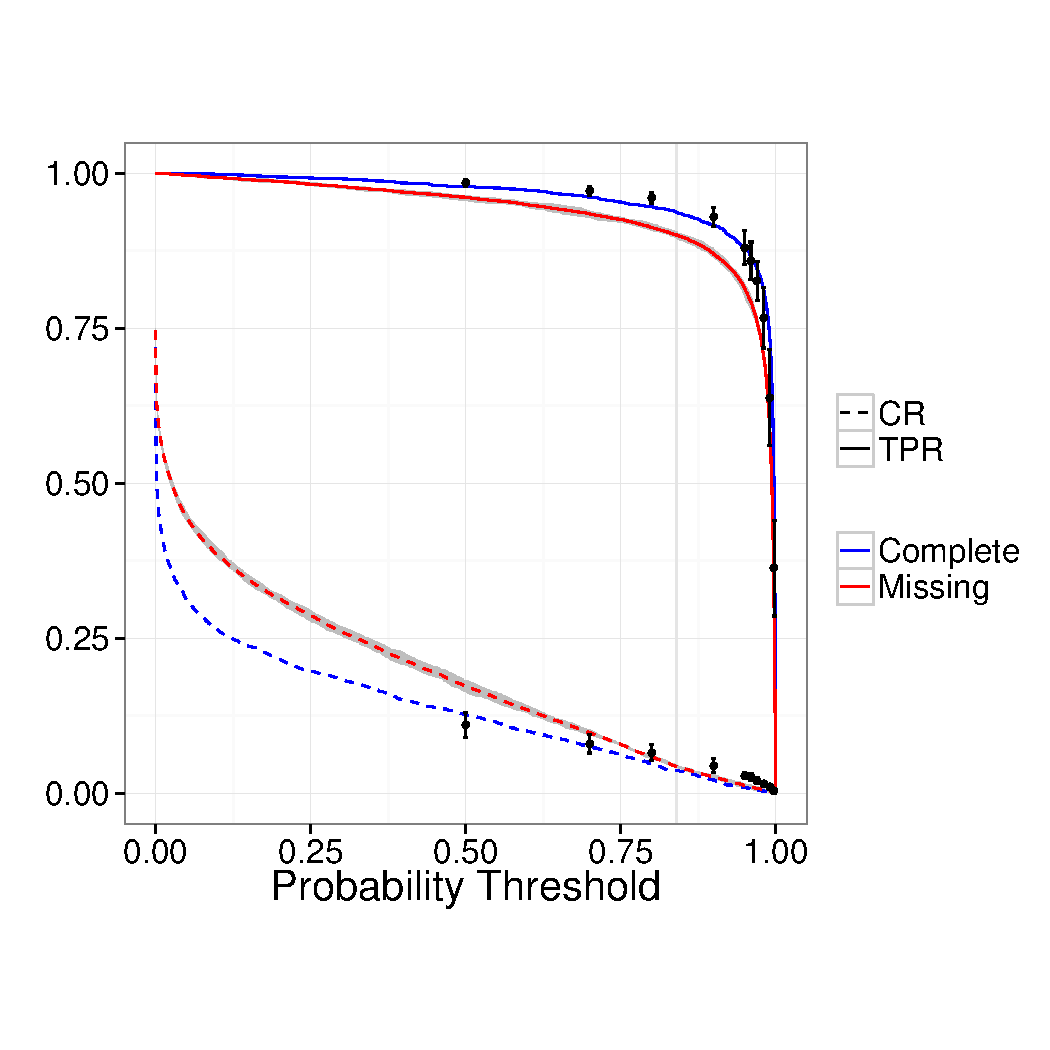
\includegraphics{background/Figures/FTPRvsSarro.pdf}}
\caption{The mean \gls{tpr} (solid line) and \gls{cr} (dashed line) resulting from five synthetic data sets including objects with missing entries (red lines). Also the \gls{tpr} and \gls{cr} resulting from a synthetic data set comprising only objects with fully observed vectors (blue lines). The shaded regions (grey) show the uncertainties computed from the five synthetic data sets. The black dots show the \gls{tpr} and \gls{cr} reported by \citet{Sarro2014} for their model. See text for warnings on this comparison. Reproduced from Figure 3 of \citet{Olivares2017},\textit{\usebibentry{Olivares2017}{Title}}, \usebibentry{Olivares2017}{Journal}, Vol. \usebibentry{Olivares2017}{Volume}.}
\label{fig:TPR-CR}
\end{center}
\end{figure}

\begin{figure}[ht!]
\begin{center}
\resizebox{0.8\textwidth}{!}{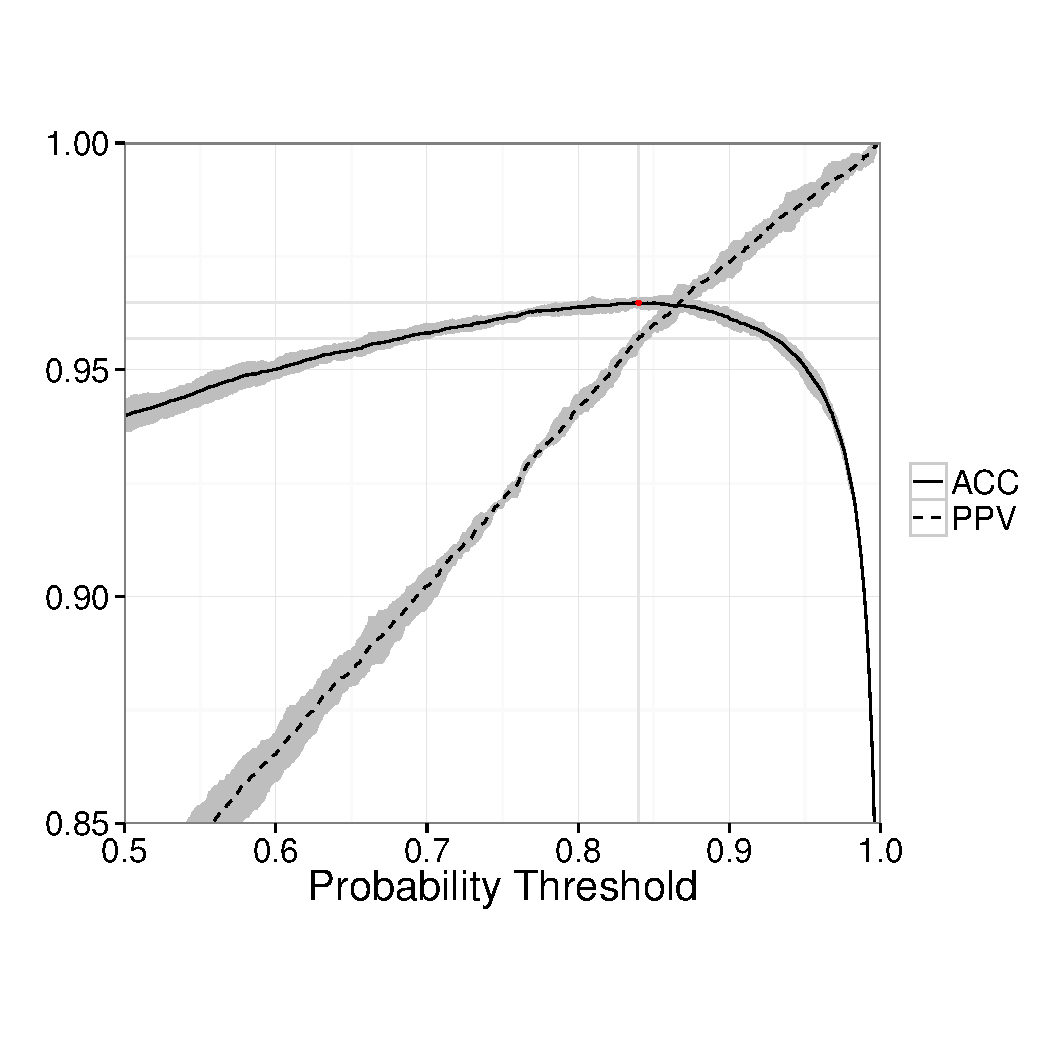
\includegraphics{background/Figures/PrecisionAccuracy.pdf}}
\caption{Mean accuracy (\gls{acc}, solid line) and precision (\gls{ppv}, dashed line) of the classifier as a function of probability threshold. The shaded regions shows the uncertainties computed from the five synthetic data sets. The higher accuracy is obtained at $p_t=0.84$ (red dot). Reproduced from Figure 3 of \citet{Olivares2017},\textit{\usebibentry{Olivares2017}{Title}}, \usebibentry{Olivares2017}{Journal}, Vol. \usebibentry{Olivares2017}{Volume}.}
\label{fig:ACC}
\end{center}
\end{figure}

We further investigate the impact that objects with missing value entries in their observations have on our methodology. In specific, I analyse possible biases introduced by these objects. To do this, I compare the membership probabilities, summarised by the mode, recovered after inferring the model on two synthetic data sets of. These two data sets are identical except that in one of them some entries in the vector of observables where masked as missing (using the procedure previously described).

In Fig. \ref{figure:IncVsCom}, I compare the mode of the membership probabilities. The horizontal axis shows the membership probabilities of the data set with fully observed objects (I call this case the complete one). The vertical axis shows the membership probabilities of the same objects but in which some entries were masked as missing (I call this case the Incomplete one). As can be seen in this figure, the missing values impact our results by spreading the membership probabilities. Ideally, we would like to recover membership probabilities following the line of slope one. This is the case of some fully observed objects (red squares) in the data set containing objects with missing entries. The most striking deviations come from those objects with the $\gls{ci}$ masked as missing (enclosed in black). The \gls{bhm} methodology uses the \emph{true} $\gls{ci}$ to prescribe the \emph{true} photometry. Also, it uses the observed $\gls{ci}$ to constrain the marginalisation integral of the \emph{true} $\gls{ci}$. Thus, as expected, a missing $\gls{ci}$ produces a spread in the membership probability. \gls{ci}

The objects with a missing $\gls{ci}$ show two different behaviours. In one case, there are objects with membership probabilities from the fully observed data set (horizontal axis) that have an overestimated membership probability in the missing entries data set (vertical axis). In the other case, there are objects that have underestimated probabilities in the missing entries data set. These objects correspond to those seen in the combed area below the line of unit slope. 

Objects in the first case increase the \gls{cr}, and their effect can be seen by the difference between red and blue dashed lines in Fig. \ref{fig:TPR-CR}. On the other hand, the objects in the second case diminish the \gls{tpr}, their effect can also be seen by the difference between red and blue solid lines in Fig. \ref{fig:TPR-CR}. The increase in \gls{cr} reaches its maximum near probability zero in the horizontal axis (Complete case) and goes to zero at probability thresholds of $\sim 0.9$. Therefore, the impact this increased \gls{cr} has in our results is marginal. For example, at the optimal probability threshold $p_t=0.84$, the increase of \gls{cr} due to objects with missing entries represent only 1.8\%. This correspond to the objects in box region of Fig. \ref{figure:IncVsCom} (upper left corner). However, the objects in the second case, those that diminish the \gls{tpr}, represent the typical unavoidable loss of members due to their missing entries. These amount to a 4\% loss in the \gls{tpr}, at the optimal probability threshold, $p_t=0.84$.


The bias introduced in the recovered membership probabilities due to objects with missing value entries, can be quantified using the root-mean-square (rms) of the difference between the means of the two recovered membership probabilities (Complete and Incomplete cases). The total rms is 0.12. On the one hand, fully observed objects in both data sets (Complete and Incomplete cases) have a rms of only 0.02. On the other hand, objects with missing entries, excluding those with missing $\gls{ci}$, have a rms of 0.08. The rms of objects lacking the $\gls{ci}$ is 0.14. The previous effects show an overall agreement between results on data sets with and without objects with missing entries. Nonetheless, care must be taken when dealing with individual membership probabilities. An object with a missing value in the $Y,J,H$ and $K_s$ may have a diminished membership probability (with a rms of 0.08), while an object with a missing $\gls{ci}$ may show an increased membership probability (with a rms of 0.14).  


However, as have been mentioned before, the methodology described in this work aims at the statistical distributions of the cluster population. The individual membership probabilities are just a useful by product. The methodology develop here, though, works by ensuring that each object contributes to the posterior distribution of the parameters modelling the cluster population, proportionally to its cluster membership probability. In this sense our results are free of any possible bias introduced by cuts in the membership probability. Nevertheless, there is still contamination. In particular, that arising from objects with missing entries. This contamination in the statistical distributions that we aim to obtain must be quantified. To do this, I compute the expected value of the \gls{cr} found in this section. It is $\langle \gls{cr} \rangle=5.8\pm 0.2$\%. In this expected value, each \gls{cr} contributes proportionally to the probability threshold at which it is measured. Since the vast contribution to this \gls{cr} coms from probability thresholds below 0.2 (see Fig. \ref{fig:TPR-CR}), the expected value of the \gls{cr} remains low. 

\begin{figure}[!htp]
\begin{center}
\resizebox{0.8\textwidth}{!}{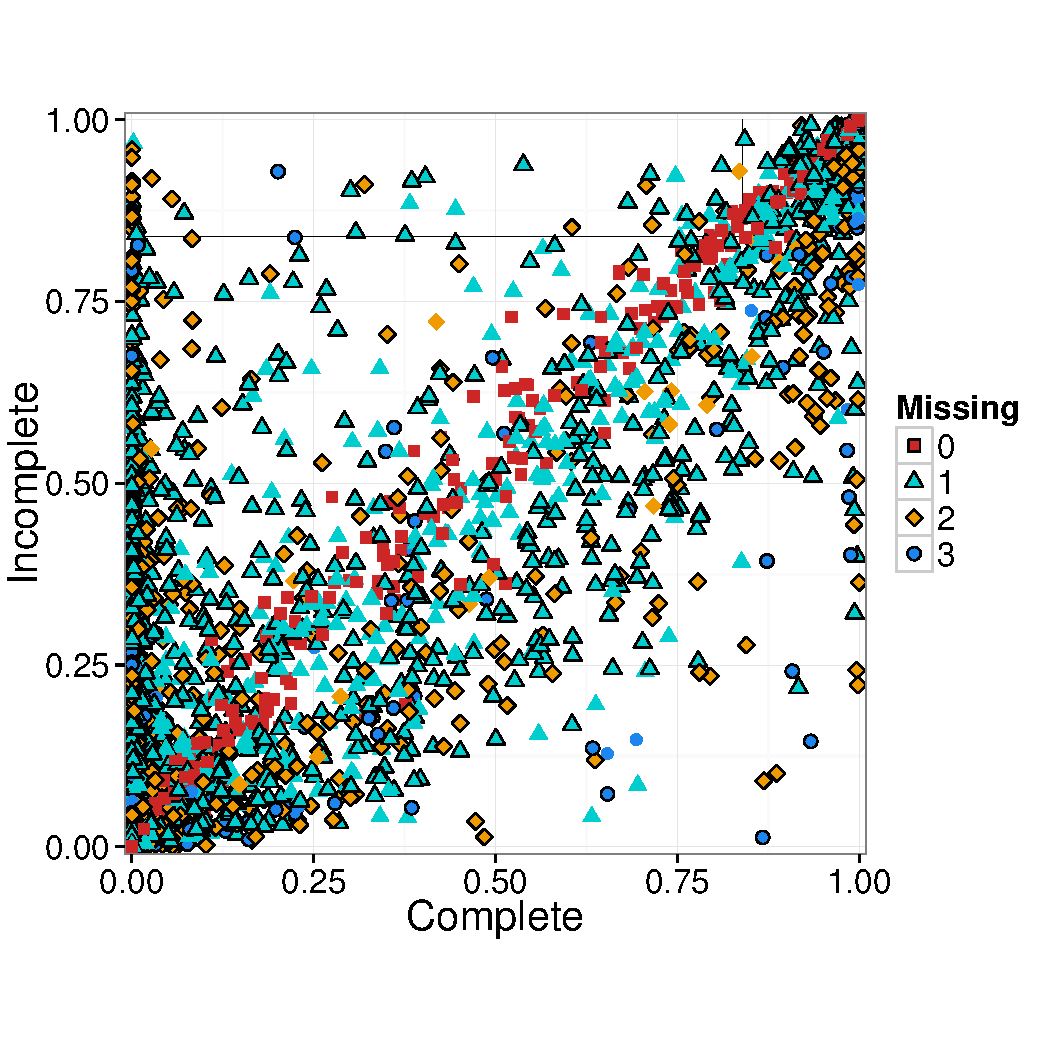
\includegraphics[page=1]{background/Figures/Probabilities.pdf}}
\caption{Comparison between the cluster membership probabilities recovered from the synthetic data set with objects having missing value entries (vertical axis, labeled Incomplete), and, the synthetic data set with fully observed objects (horizontal axis, labeled Complete). The colour and shape indicate the amount of missing entries. The symbols enclosed in black indicate a missing $\gls{ci}$. The top left box contains objects considered as contaminants due to missing values at the probability threshold $p_t=0.84$. Reproduced from Figure 4 of \citet{Olivares2017},\textit{\usebibentry{Olivares2017}{Title}}, \usebibentry{Olivares2017}{Journal}, Vol. \usebibentry{Olivares2017}{Volume}.}
\label{figure:IncVsCom}
\end{center}
\end{figure}

In statistical science,  in machine learning particularly, is sometimes useful to analyse the performance of a binary classifier by the receiver operating characteristic curve, the \gls{roc} curve. It plots a visual diagnostic of the ability of a classifier to perform its job. The \gls{roc} curve plots the \gls{tpr} as a function of the \gls{fpr} for all possible values of the probability threshold. A perfect classifier would be that in which the \gls{tpr}=1 and the \gls{fpr}=0 for some probability threshold. On the other hand, a random classifier would be that with \gls{tpr}=\gls{fpr} at all probability thresholds. Such classifier has a line of slope one in its \gls{roc} curve. Furthermore, the quantitative diagnostic for a binary classifier is the \gls{auc} \gls{roc}. As its name indicate, the \gls{auc} is the integral of the \gls{roc} curve. Thus a random classifier has a \gls{auc} of one half, while a perfect classifier has a \gls{auc}=1. In Fig. \ref{fig:ROC}, I show the \gls{roc} curve for our classifier when applied over synthetic data containing objects with missing entries. It is the \gls{roc} of one of the five synthetic realisations described throughout this section. As can bee seen from this Figure our classifier does an excellent job, with an \gls{auc}=0.992.

\begin{figure}[!htp]
\begin{center}
\resizebox{0.8\textwidth}{!}{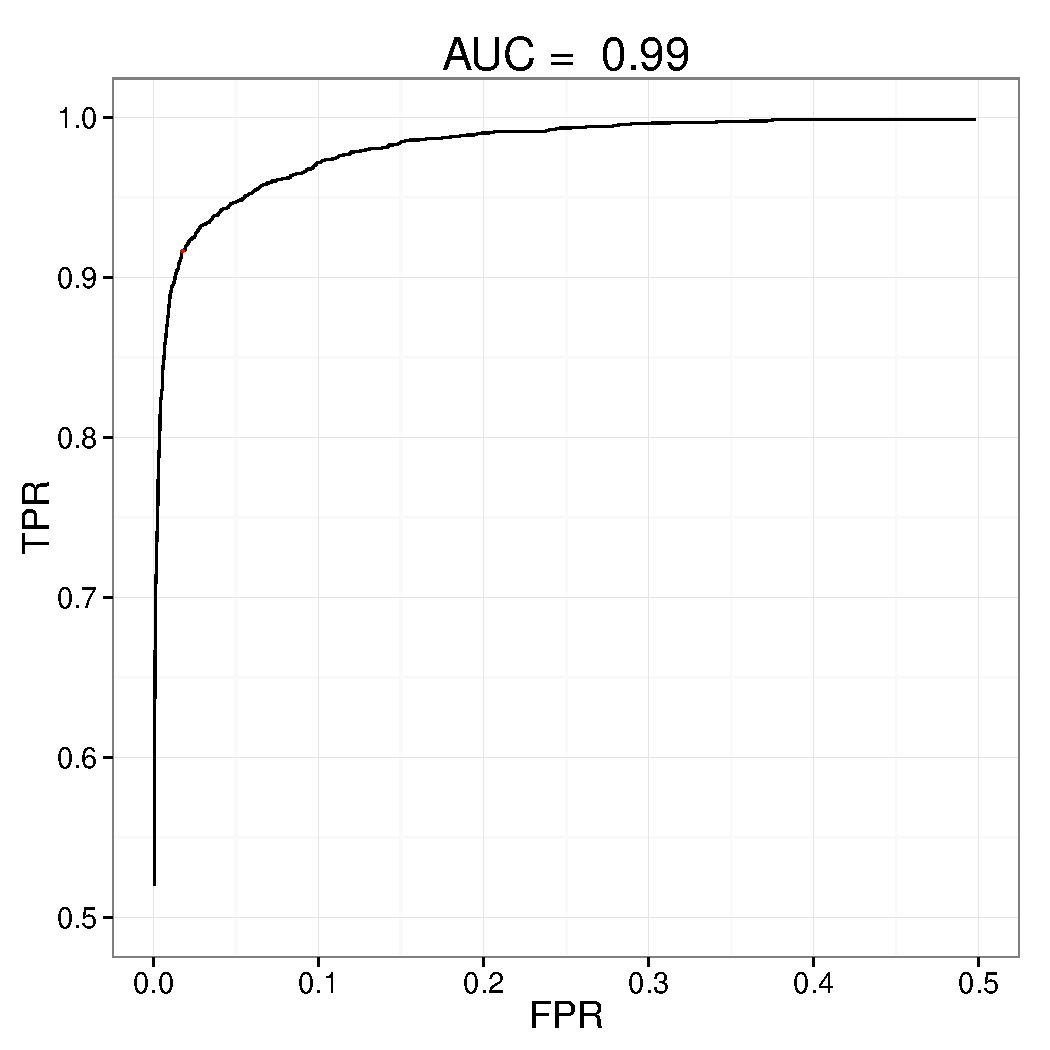
\includegraphics{background/Figures/ROC.pdf}}
\caption{\gls{roc} curve of the \gls{bhm} by-product classifier when applied on the synthetic data set containing objects with missing entries. As can be seen, the \gls{auc}=0.992 diagnose it as an excellent classifier.}
\label{fig:ROC}
\end{center}
\end{figure}

 
\section{Comparison with the literature}
\label{sect:memberscomparison}

The \gls{bhm} methodology, described in Chapter \ref{chap:BHM}, is applied to the \gls{rdr2}. Then, I compare the recovered membership probabilities with those reported in the literature. The first comparison I present is that of our candidate members with those in the two lists of candidate members of \citet{Stauffer2007}. Then, I proceed to compare our membership probabilities with those found by \citet{Bouy2015}. Finally, I compare the candidate members recovered by the \gls{bhm} with those found by \citet{Rebull2016}. These authors obtain their list of candidates based on photometric variability. This observable is not present in our set of observables, for this reason this comparison represent an extra source of external validation.  


\subsection{Candidate members from \citet{Stauffer2007}}

\citet{Stauffer2007} published two list of candidate members. The first one contains 1417 objects compiled from the literature (see Table 2 of the mentioned work). These objects were classified as candidate members by several authors. As \citet{Stauffer2007} mention, this list is inhomogeneous, incomplete and certainly includes non-members. I refer to this list as \gls{st1}. Their second list contains 55 candidate members (see Table 5 of the mentioned work). \citet{Stauffer2007} found these members using infrared photometry and proper motions. I refer to this list as \gls{st2}.

Cross matching (at CDS\footnote{ Using the service http://cdsxmatch.u-strasbg.fr/xmatch}, within 1 arcsec radius) the previous two lists with the \gls{ddr2} catalogue \citep{Bouy2015}, I find that only 1384 and 54 of the \gls{st1} and \gls{st2} lists have a counter part in the \gls{ddr2} catalogue, respectively. 

Concerning our list of candidate members, after cross matching it with the two lists of \citet{Stauffer2007}, \gls{st1} and \gls{st2}, I recover 1146 and 34 of the candidate members, respectively. Compared to the candidate members of \citet{Bouy2015}, our \gls{bhm} recovers 28 more candidate members in \gls{st1} and the same in \gls{st2}.

As mentioned before, the \gls{st1} list is an exhaustive compilation of Pleiades members. It contains objects that were classified, at some point in history, as Pleiades candidate members, even when their membership probability are as low as 0.1 \citep{Stauffer2007}. For this reason I will not analyse the details of 238 rejected objects of \gls{st1}. It suffices to show that these rejected objects lie far from the cluster photometric or proper motions loci, as shown in Fig. \ref{fig:ST1}.

On the other hand, from the 20 objects in \gls{st2} that are rejected by the \gls{bhm}, 18 of them lie below the cluster photometric sequence and far from the proper motion locus, see Fig. \ref{fig:ST2}. The remaining two (\gls{dance} IDs: J034552.57+235145.9 and J034543.47+233851.5), although have observed photometric vectors compatible with the clusters sequence, their proper motions still are far from the cluster centre (with $\mu_{\alpha}\cos(\delta)\sim 40\,\rm{mas\cdot yr^{-1}}$), see Fig. \ref{fig:ST2}.

\begin{figure}[ht!]
    \centering
    \begin{subfigure}[t]{0.45\textwidth}
    \centering
       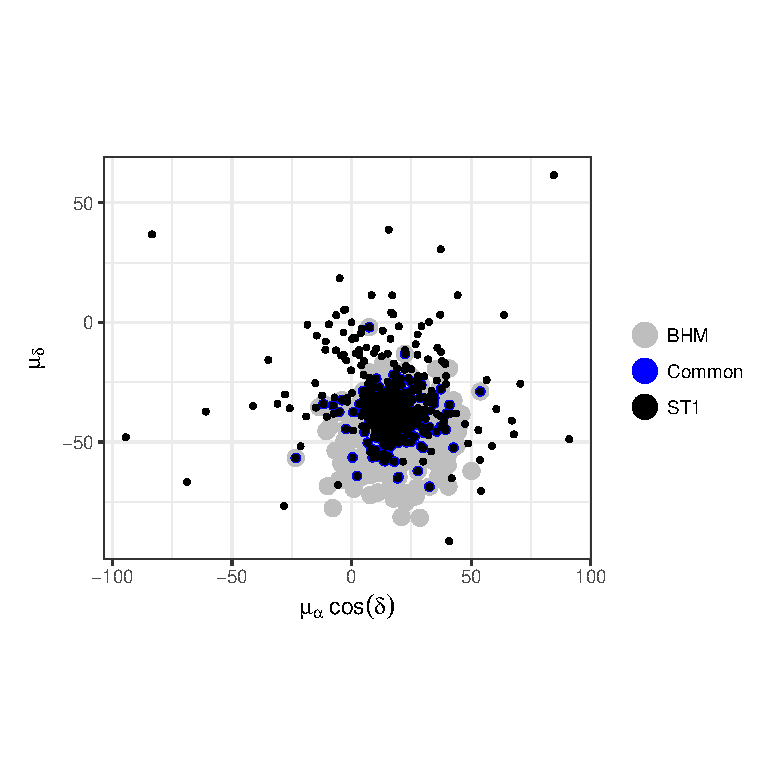
\includegraphics[width=\textwidth]{background/Figures/ST1_pm.eps}
        \caption{}
    \end{subfigure}
    \begin{subfigure}[t]{0.45\textwidth}
    \centering
     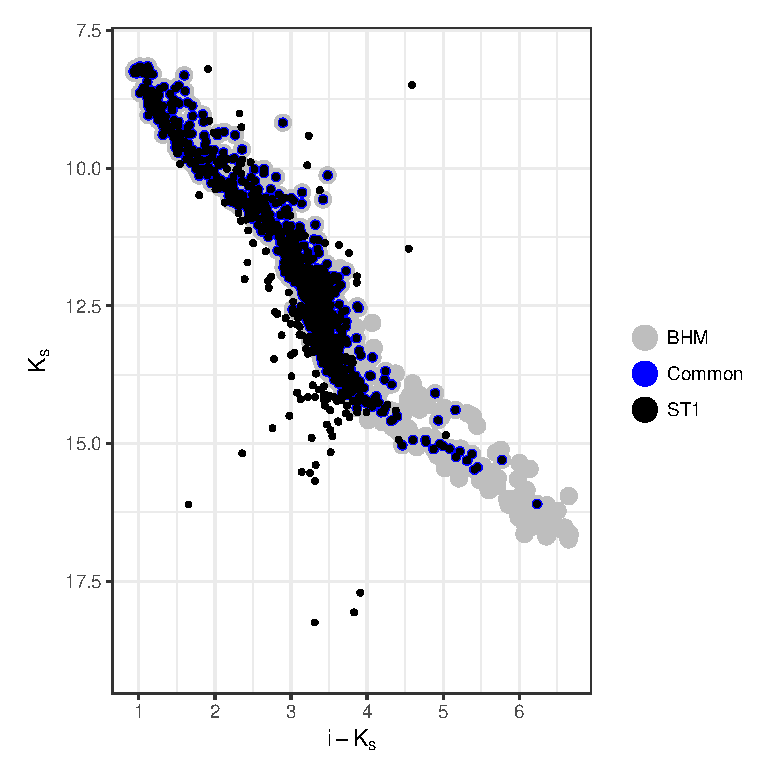
\includegraphics[width=\textwidth]{background/Figures/ST1_ph.eps}
        \caption{}
    \end{subfigure}
\caption{Proper motions (a) and $K$ vs $i-K$ \gls{cmd} (b) of the \gls{st1} candidate members in the \gls{ddr2} catalogue (black). Also shown, the objects classified as candidate members  in the \gls{bhm} (grey), and in both \gls{st1} and \gls{bhm} (blue).}
\label{fig:ST1}
\end{figure}

\begin{figure}[ht!]
    \centering
    \begin{subfigure}[t]{0.45\textwidth}
    \centering
       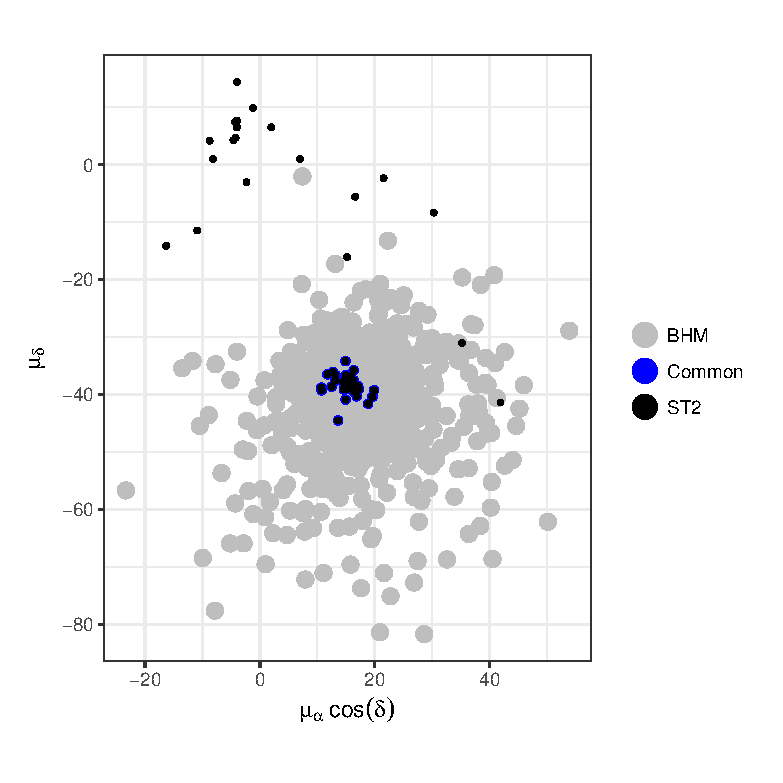
\includegraphics[width=\textwidth]{background/Figures/ST2_pm.eps}
    \end{subfigure}
    \begin{subfigure}[t]{0.45\textwidth}
    \centering
     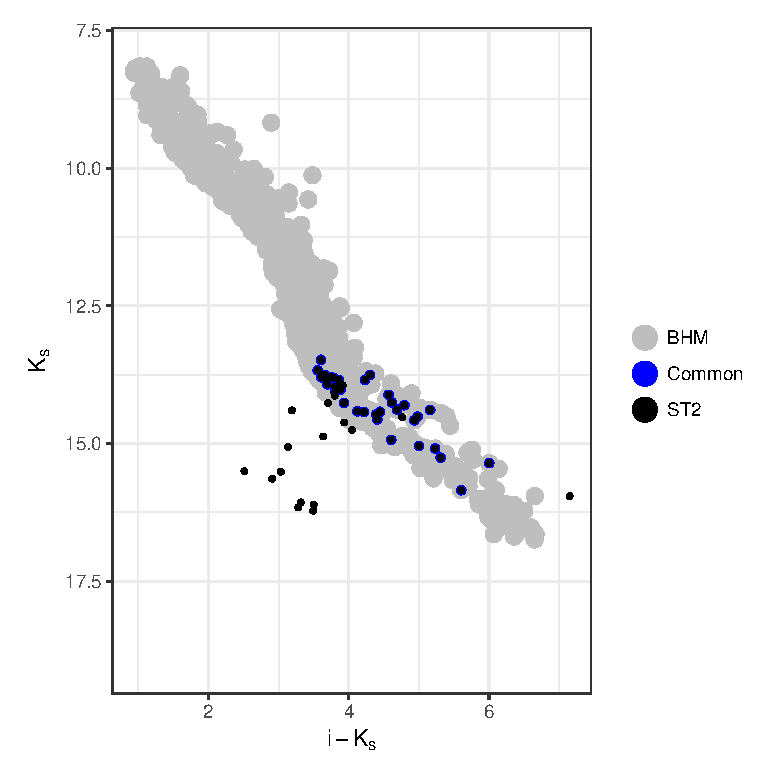
\includegraphics[width=\textwidth]{background/Figures/ST2_ph.eps}
        \caption{}
    \end{subfigure}
\caption{Proper motions (a) and $K$ vs $i-K$ \gls{cmd} (b) of the \gls{st2} candidate members in the \gls{ddr2} catalogue (black). Also shown, the objects classified as candidate members in the \gls{bhm} (grey), and in  both \gls{st2} and \gls{bhm} (blue).}
\label{fig:ST2}
\end{figure}

\subsection{Candidate members from \citet{Bouy2015}}
\label{sect:comparisonBouy}

The fact that the work of \citet{Bouy2015} and the present one use the same \gls{ddr2} data set (although our model is constructed with the \gls{rdr2}), allow me to directly compare the membership probabilities of both works. Furthermore, this comparison can be extended to all objects in the data set and not just to the candidate members of the Pleiades cluster. Since \citet{Bouy2015} reported only an statistic of the membership probability distributions, to do a fair comparison, I summarise the membership probability distributions recovered by the \gls{bhm} with the mode.

Using the optimal probability threshold of 0.84 to classify the cluster members, we can see that, as shown by Fig. \ref{fig:BHMBouy}, both methodologies agree on the outstanding $99.6$\% of the classified objects. Concerning just the candidate members, the agreement is still high, $\sim 90\%$. In the following I discuss the 10\% discrepancies.

\begin{figure}[ht!]
\begin{center}
\resizebox{\textwidth}{!}{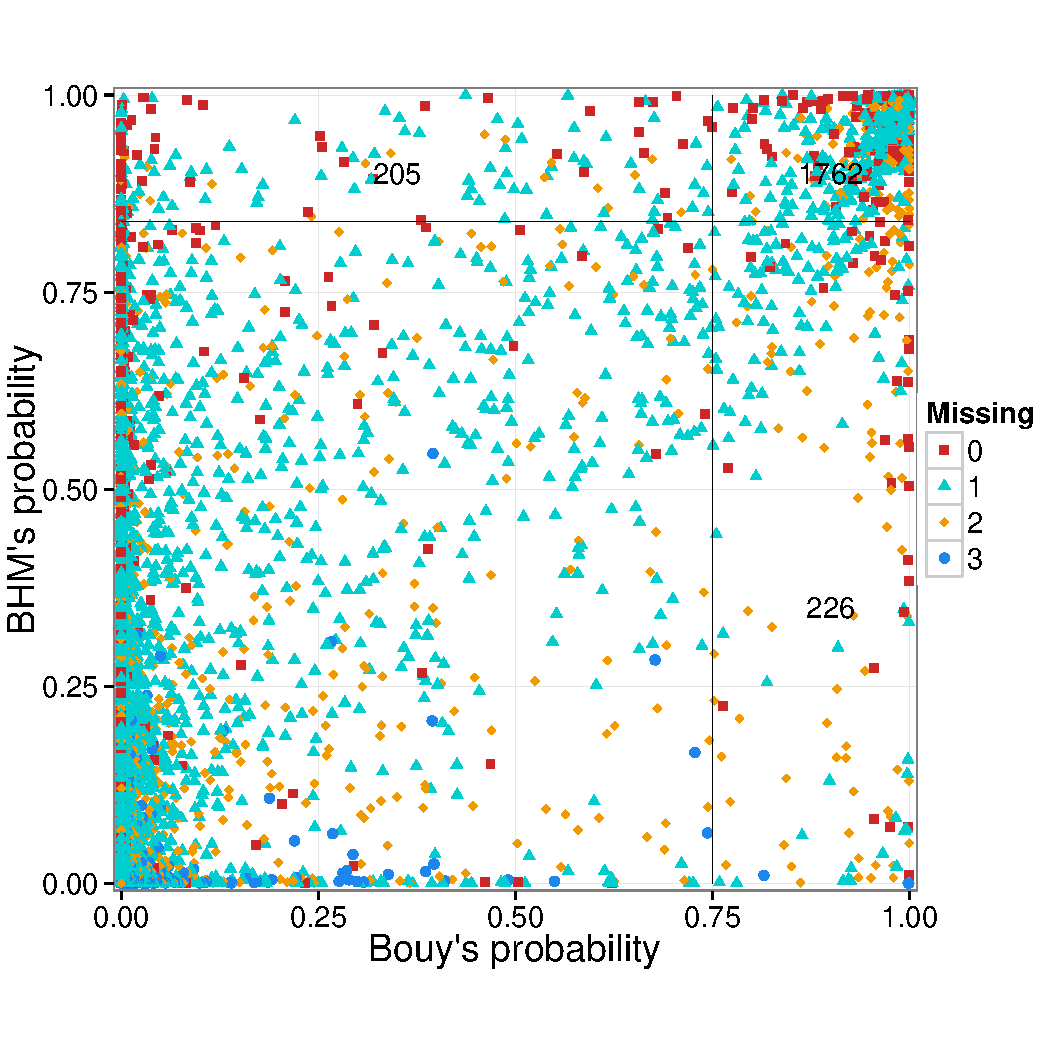
\includegraphics{background/Figures/BHM/BHMvsBouy.pdf}}
\caption{Mode of the membership probabilities recovered by the \gls{bhm} compared to those of \citet{Bouy2015}. The lines show the 0.75 and $p_t=0.84$ probability thresholds used in both works. The numbers indicate our new candidate members (top left), the ones we rejected (bottom right), and the common ones (top right). Reproduced from Figure 11 of \citet{Olivares2017},\textit{\usebibentry{Olivares2017}{Title}}, \usebibentry{Olivares2017}{Journal}, Vol. \usebibentry{Olivares2017}{Volume}.}
\label{fig:BHMBouy}
\end{center}
\end{figure}

The candidate members of \citet{Bouy2015} that the \gls{bhm} rejects, which I call the rejected ones, are shown in lower right box of Fig. \ref{fig:BHMBouy}. They amount to 12\% and 12.5\% of total number of candidate members recovered by \citet{Bouy2015} and the present work, respectively. The 12\% figure is 4.7\% higher than the \gls{cr} reported by \citet{Sarro2014} ($7.3\pm1.4$\%). It indicates that some true cluster members must be within the rejected objects. Also, the 12.5\% figure is 2.5\% higher than the 10\% loss rate of the \gls{bhm} (\gls{tpr}=90\%, see Section \ref{sect:classifier}), which indicates that some contaminants must be within the rejected objects.

Now, I analyse these objects with further detail. As it is shown in Figs. \ref{fig:rejecteds} and \ref{fig:rejectedsCOLORS}, the rejected objects have proper motions uncertainties with median $\tilde{\mu}_{\alpha},\tilde{\mu}_{\delta}=\{3.19,3.20\} \,\mathrm{mas\cdot yr^{-1}}$. This value is more than four times larger than that of the common candidate members (those objects classified as members by both works, see top right corner of Fig. \ref{fig:BHMBouy}), which have median $\tilde{\mu}_{\alpha},\tilde{\mu}_{\delta}=\{0.68,0.68\} \,\mathrm{mas\cdot yr^{-1}}$. Among the rejected ones, those with a relatively high membership probability occur mostly at the middle of the cluster photometric sequence (green squares of Fig. \ref{fig:rejectedsCOLORS}). On the other hand, those with lower membership probabilities occur at the bright and faint ends (blue and red triangles of Fig. \ref{fig:rejectedsCOLORS}, respectively). Furthermore, the proper motions uncertainties of the rejected objects at the bright, middle and faint ends of the cluster photometric sequence, have medians of $\tilde{\mu}_{\alpha},\tilde{\mu}_{\delta}=\{4.3,4.2\}  \,\mathrm{mas\cdot yr^{-1}}$, $\tilde{\mu}_{\alpha},\tilde{\mu}_{\delta}=\{2.4,2.4\}\,\mathrm{mas\cdot yr^{-1}}$ and $\tilde{\mu}_{\alpha},\tilde{\mu}_{\delta}=\{3.4,3.4\}\,\mathrm{mas\cdot yr^{-1}}$, respectively. These figures are approximately 6, 4 and 5 times larger, respectively, than those of the candidates in common. These large uncertainties produce a proportional spread of the cluster likelihood. This could reduce the membership probability of these objects.

Furthermore, the bright and faint regions of the cluster photometric sequence coincide with those where objects with missing entries are more frequent (see Fig. \ref{fig:NAsKs}). I stress the fact that the model of \citet{Bouy2015} was constructed using only objects with fully observed vectors of measurements, which represent less than 1\% of the number of objects used by the \gls{bhm}. Using only fully observed objects, underestimates the field density in the regions where the missing values are more frequent. Underestimating the field likelihood increases the cluster to field likelihood ratio. Therefore it increases also the cluster membership probabilities. This may explain the relatively high membership probabilities reported by \citet{Bouy2015} compared to those of the \gls{bhm}. In particular, those in the faint region of the photometric cluster sequence. 

Therefore, I consider that both previous phenomena, the large proper motion uncertainties of the rejected objects together with the underestimated field likelihood in \citet{Bouy2015} model, are responsible for the relatively lower \gls{bhm} membership probabilities of the rejected objects. However, these objects can not be discarded as potential true cluster members. To discard this possibility lower proper motion uncertainties and fewer missing values are needed. Future steps will be taken to try to solve this issue.

 \begin{figure}[ht!]
\begin{center}
\resizebox{\textwidth}{!}{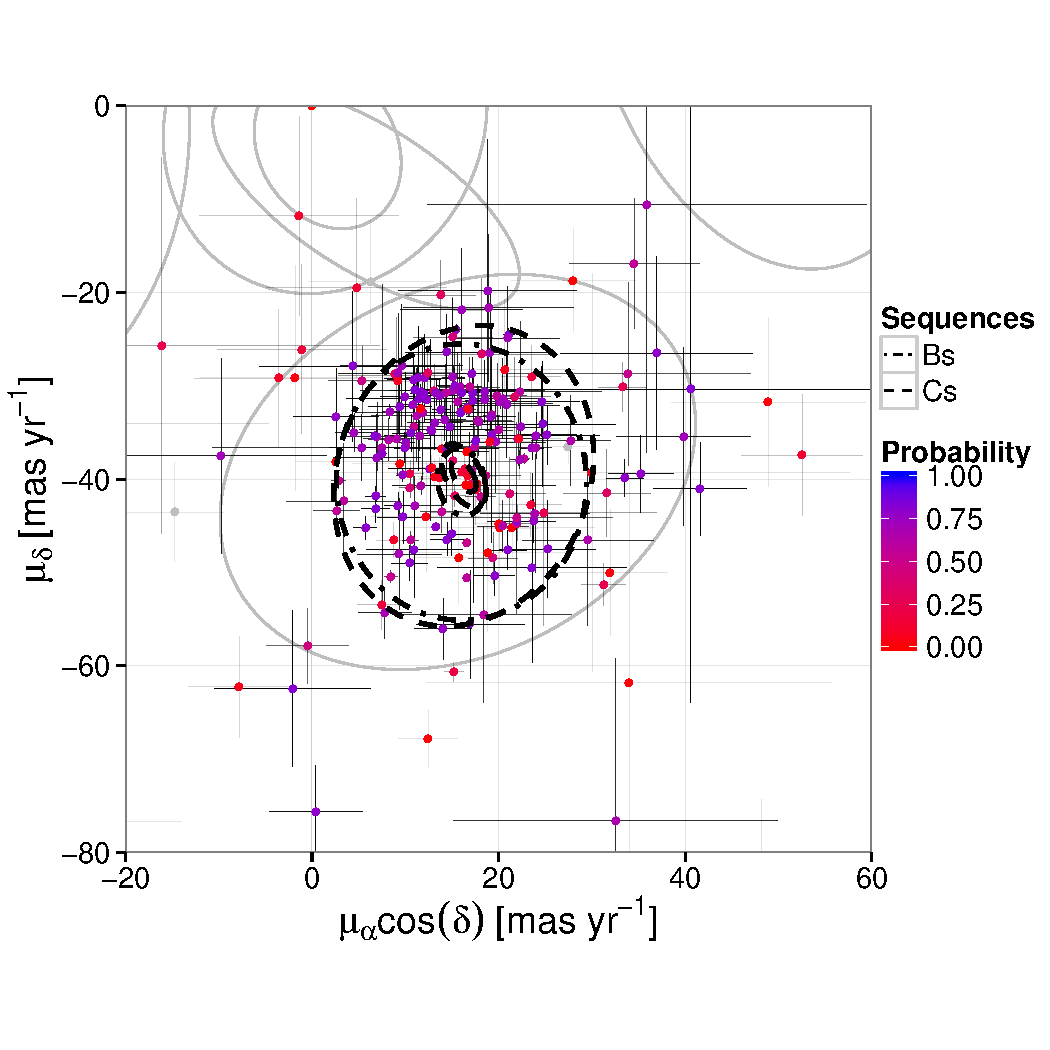
\includegraphics[page=1]{background/Figures/BHM/Rejecteds.pdf}\includegraphics[page=5]{background/Figures/Rejecteds.pdf}}
\caption{Proper motion (left) and $K_s$ vs. $i-K_s$ \gls{cmd} (right) showing the candidate members of \citet{Bouy2015} rejected by the \gls{bhm}. Reproduced from Figure 13 of \citet{Olivares2017},\textit{\usebibentry{Olivares2017}{Title}}, \usebibentry{Olivares2017}{Journal}, Vol. \usebibentry{Olivares2017}{Volume}.}
\label{fig:rejecteds}
\end{center}
\end{figure}

\begin{figure}[htbp]
\begin{center}
\resizebox{\hsize}{!}{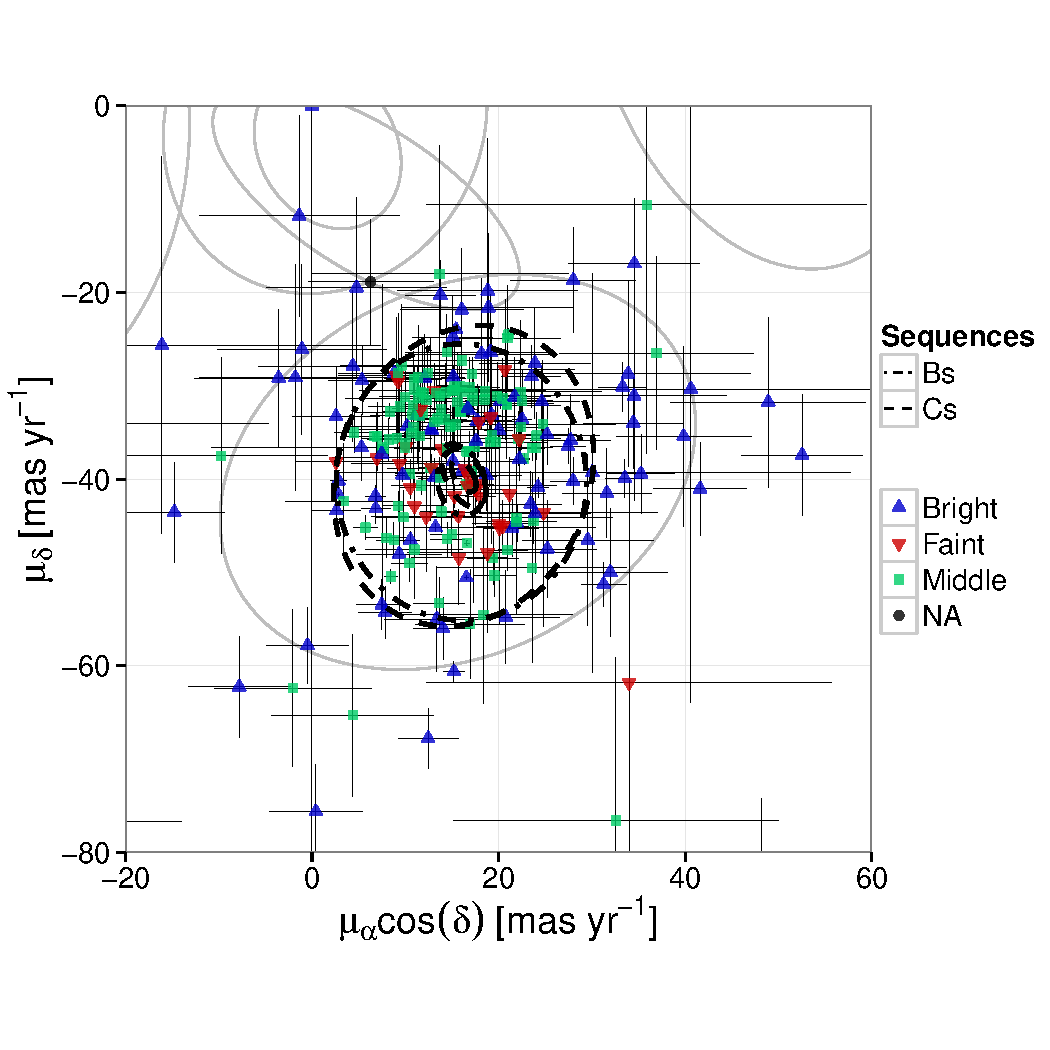
\includegraphics[page=1]{background/Figures/BHM/RejectedsCOLORS.pdf}\includegraphics[page=5]{background/Figures/RejectedsCOLORS.pdf}}
\caption{Proper motion (left) and $K_s$ vs. $i-K_s$ \gls{cmd} (right) showing the candidate members of \citet{Bouy2015} rejected by the \gls{bhm}. The colours and shapes are a proxy for their $K_s$ magnitude.Reproduced from Figure 14 of \citet{Olivares2017},\textit{\usebibentry{Olivares2017}{Title}}, \usebibentry{Olivares2017}{Journal}, Vol. \usebibentry{Olivares2017}{Volume}.}
\label{fig:rejectedsCOLORS}
\end{center}
\end{figure}

On the other hand, the new candidates members found by the \gls{bhm}, shown in the upper left box of Fig. \ref{fig:BHMBouy}, amount to 10\% of the \citet{Bouy2015} candidate members. This figure is higher than the $\sim 3.5\%$ of missing rate (1-\gls{tpr}) reported by \citet{Sarro2014}. Also, these new candidates amount to 10\% of the \gls{bhm} recovered candidate members. This value is larger than the 4.3\% \gls{cr} reported in Section \ref{sect:classifier}. These two larger figures may indicate that some truly new discoveries may be within these list of new candidate members. In Figs. \ref{fig:newones} I show the proper motions and $K_s$ vs $i-K_s$ \gls{cmd} of these new candidates members.

The new candidate members have proper motions uncertainties whose median, $\tilde{\mu}_{\alpha},\tilde{\mu}_{\delta}=\{1.41,1.41\} \,\mathrm{mas\cdot yr^{-1}}$, is two times larger than those of the candidate members in common with \citet{Bouy2015}. Also, as shown by Fig. \ref{fig:newones}, the majority of the new candidate members, 166, have probabilities lower than 0.95, are located in a halo around the locus of the cluster proper motions, and on top of the cluster photometric sequence in the $K_s$ vs $i-K_s$ \gls{cmd}. On the contrary, the new candidate members with probabilities higher than 0.95, which are 39, lie in the centre of the cluster proper motions and fall above the cluster sequence in the $K_s$ vs $i-K_s$ \gls{cmd}. Thus, I hypothesise that: i) Objects whose photometry is compatible with the cluster sequence but are in the proper motions halo, have higher membership probabilities in our methodology due to the increased flexibility of the cluster proper motions model: it now has four gaussians instead of the two of \citet{Bouy2015}. And ii) objects near the centre of the cluster proper motions but located above the cluster photometric sequence sequence, are multiple systems \cite[probably triple systems which can amount to 4\% of the population][]{Duquennoy1991} with an increased membership probability due to our more flexible photometric model of the cluster and equal-mass binaries sequences.

 \begin{figure}[ht]
\begin{center}
\resizebox{\hsize}{!}{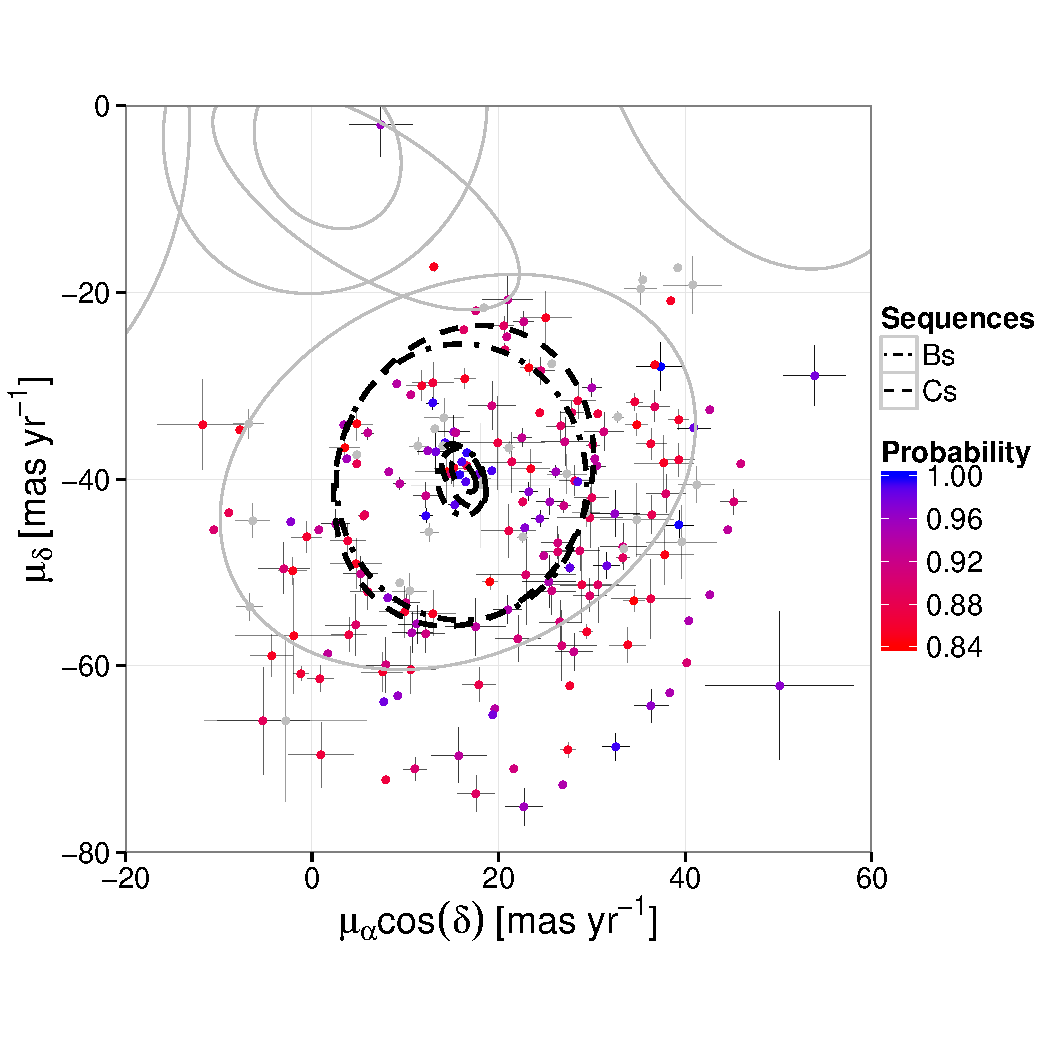
\includegraphics[page=1]{background/Figures/BHM/NewOnes.pdf}\includegraphics[page=5]{background/Figures/NewOnes.pdf}}
\caption{Proper motion (left) and $K_s$ vs. $i-K_s$ \gls{cmd} (right) showing the new candidate members found in this work. Reproduced from Figure 12 of \citet{Olivares2017},\textit{\usebibentry{Olivares2017}{Title}}, \usebibentry{Olivares2017}{Journal}, Vol. \usebibentry{Olivares2017}{Volume}.}
\label{fig:newones}
\end{center}
\end{figure}


Summarising, the discrepancies between the \gls{bhm} membership probabilities and those reported by \citet{Bouy2015} arise from subtle but important differences. The first difference is the treatment of object with missing entries. Although  \citet{Bouy2015} report membership probabilities for this kind of objects, their field and cluster models were constructed discarding them. This may have biased their results. Taking into account objects with missing entries has two consequences. First, the photometric model is more accurate than any other model that discards objects with missing entries. This effect is important in the regions where these objects are more frequent. Second, the use of objects with missing entries in the construction of the cluster model allow us to include the information of good candidate members that were otherwise discarded a priori. A second difference with the model of \citet{Bouy2015}, is the higher flexibility of our cluster model. It allows us to increase the membership probability of the previously discarded candidates. 

\subsection{Candidate members from \citet{Rebull2016}}
\label{sect:comparisonRebull}

After cross matching (at CDS with a 0.5 arcsec radius) the list of candidate members from \citet{Rebull2016} (their Table 2, here after \gls{rt1}) with the  \gls{ddr2}, I find that 758 out of the 759 objects have a counter part in the \gls{ddr2} catalogue. The 91\% of these objects (690 of them) are candidate members in the \gls{bhm}. Under the assumption that the candidate members in \gls{rt1} are indeed true members, which may not be true, the ratio of recovered members is even better than the $\gls{tpr}=90\pm0.2\%$ reported in Section \ref{sect:classifier}. These objects are shown in Fig. \ref{fig:RT1}.

\begin{figure}[ht!]
    \centering
    \begin{subfigure}[t]{0.45\textwidth}
    \centering
       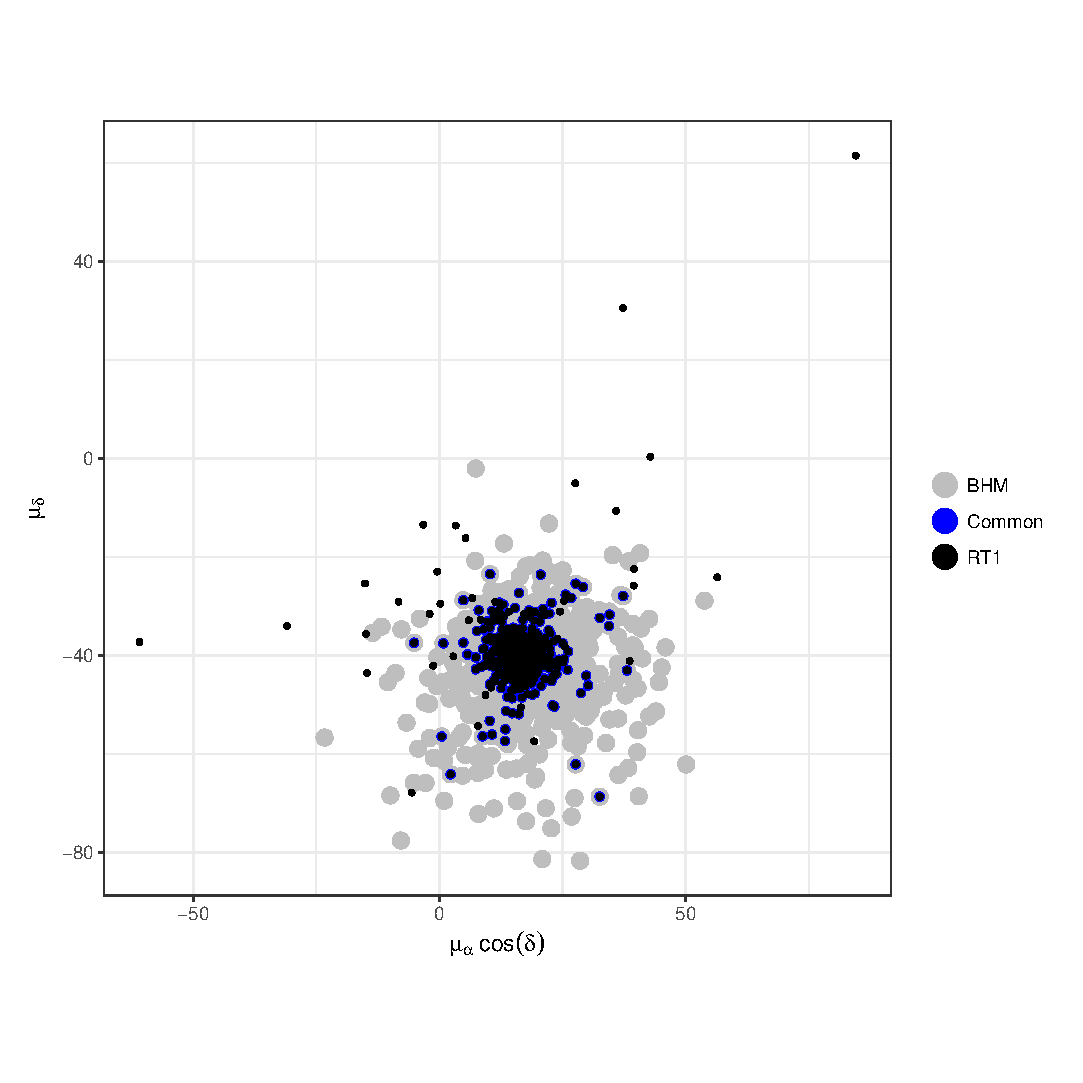
\includegraphics[width=\textwidth]{background/Figures/RT1_pm.eps}
        \caption{}
    \end{subfigure}
    \begin{subfigure}[t]{0.45\textwidth}
    \centering
     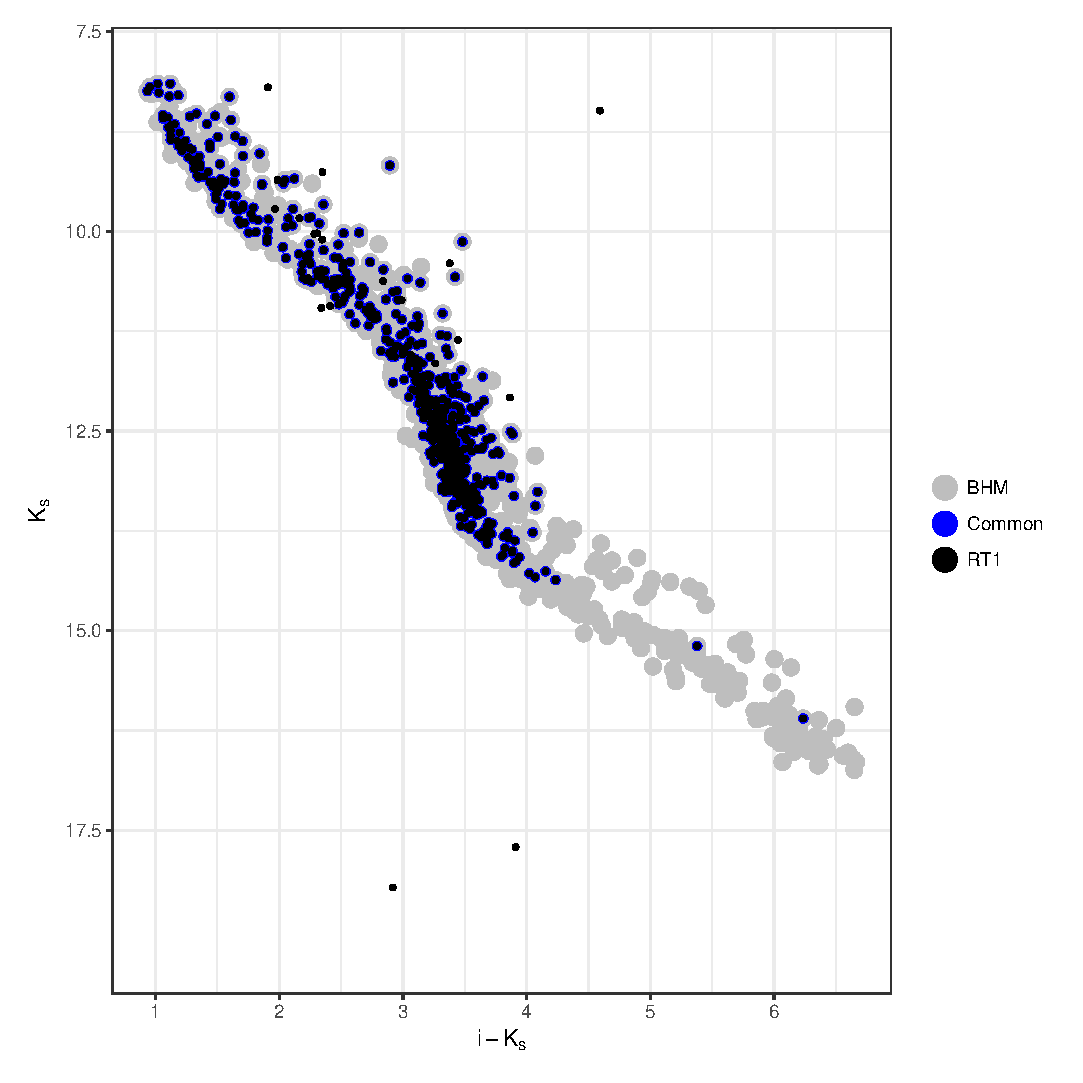
\includegraphics[width=\textwidth]{background/Figures/RT1_ph.eps}
        \caption{}
    \end{subfigure}
\caption{Proper motions (a) and $K$ vs $i-K$ \gls{cmd} (b) of the \gls{rt1} candidate members in the \gls{ddr2} catalogue (black). Also shown, the objects classified as candidate members  in the \gls{bhm} (grey), and in both \gls{rt1} and \gls{bhm} (blue).}
\label{fig:RT1}
\end{figure}

On the other hand, after cross matching (at CDS with a 0.5 arcsec radius)  the list of 154 objects that \citet{Rebull2016} classify as non-members (their Table 6, here after \gls{rt2}) with the \gls{ddr2}, I find that all these objects have a counter part on the \gls{ddr2}. The 21\% of objects in the \gls{rt2} list (33 of them) were classified as candidate members in the \gls{bhm}. This is a value five times larger than the \gls{cr} reported in Section \ref{sect:classifier} (\gls{cr}=4.3\%). However, we can not assume that the \gls{rt2} list comprises only non-members. First, this objects were at some point classified as members by other authors \cite[Appendix B of][]{Rebull2016}. Second, not all of these objects have periods \cite[only 20\% according to][]{Rebull2016}. From the 33 objects classified as candidate members by the \gls{bhm}, only nine of them have periods. It means that for the remaining 24 candidate members, these authors used other criteria to discard them as members. About their classification process, \citet{Rebull2016} say ``This process was qualitative in the sense that we weighted all of the information in a subjective manner. However, the process was also extensive, with each star considered individually and with all available information considered in detail. [...] we believe that in the great majority of cases we have made the right decision.'' In any case, the high rate of \gls{bhm} candidate members found in this \gls{rt2} list may indicate that either our contamination rate is underestimated or that the criteria used by \citet{Rebull2016} are too restrictive. As can be seen in Fig. \ref{fig:RT2}, these 33 objects have proper motions and photometric measurements consistent with those of the cluster. In order to clarify the status of these objects, further information is still needed.

\begin{figure}[ht!]
    \centering
    \begin{subfigure}[t]{0.45\textwidth}
    \centering
       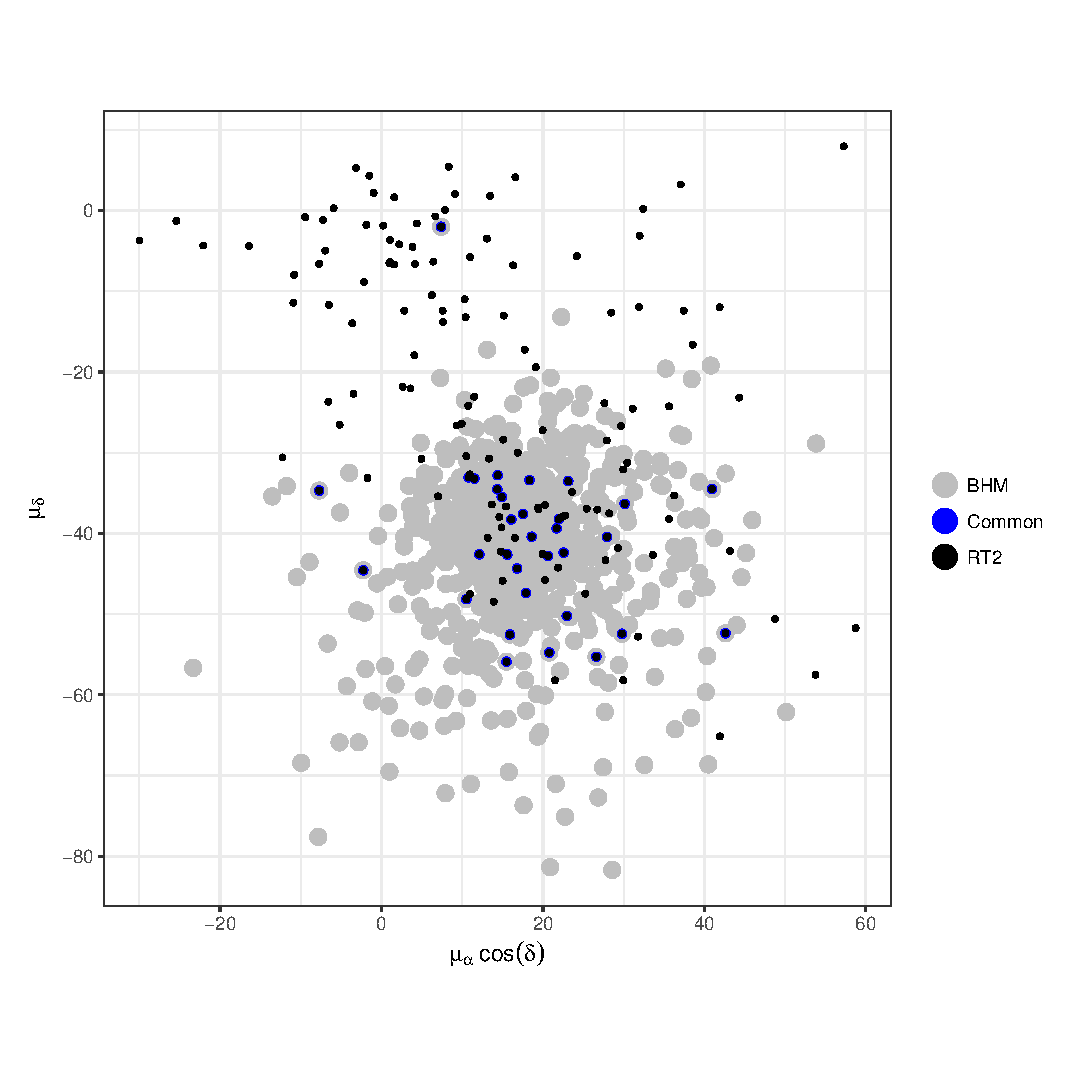
\includegraphics[width=\textwidth]{background/Figures/RT2_pm.eps}
        \caption{}
    \end{subfigure}
    \begin{subfigure}[t]{0.45\textwidth}
    \centering
     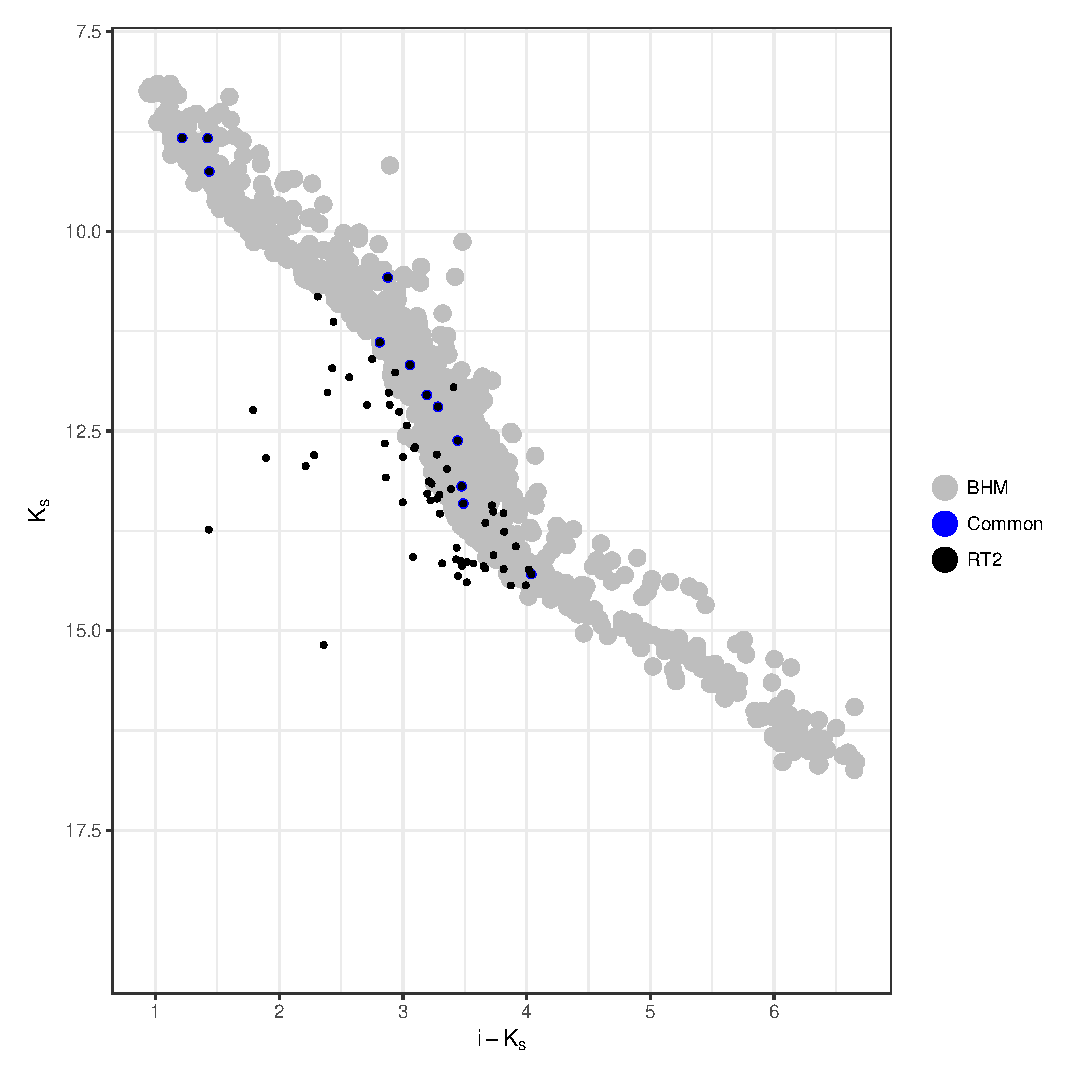
\includegraphics[width=\textwidth]{background/Figures/RT2_ph.eps}
        \caption{}
    \end{subfigure}
\caption{Proper motions (a) and $K$ vs $i-K$ \gls{cmd} (b) of the \gls{rt2} in the \gls{ddr2} catalogue (black). Also shown, the objects classified as candidate members in the \gls{bhm} (grey), and those classified as non-members in the \gls{rt2} and as candidate members in the \gls{bhm} (blue).}
\label{fig:RT2}
\end{figure}
 
\section{The statistical distributions of the Pleiades cluster.}
Now, I present the results of the statistical distributions that describe the cluster population, which are the main objective of the present work. These distributions result directly or indirectly from the posterior distribution of the parameters in our model. Indirectly means that I use them as parameters of other function (e.g. the mass distribution). Since we have 85 parameters in the \gls{bhm}, I only discuss the posterior distributions of some of these parameters. In particular, those related with the velocity, luminosity and mass distributions. Nevertheless, in Table \ref{tab:parameters}, I summarise the posterior distribution of the parameters in our model using the mode, also I use the 16th and 84th percentiles as a proxy for the uncertainty. The parameter names in this Table correspond to those given in Section \ref{sect:priors} (at Table \ref{tab:priors_parameters}). 

\textbf{The posterior distributions of the parameters in the \glspl{bspline} and the \emph{true} \gls{ci} distribution are shown in Figs. \ref{fig:CMDs_results} and \ref{fig:CI_results}, respectively.  The posterior distributions of the parameters in the proper motion models are described in Section \ref{sect:PMresults}.}

\begin{figure}[ht!]
    \centering
    \begin{subfigure}[t]{0.48\textwidth}
        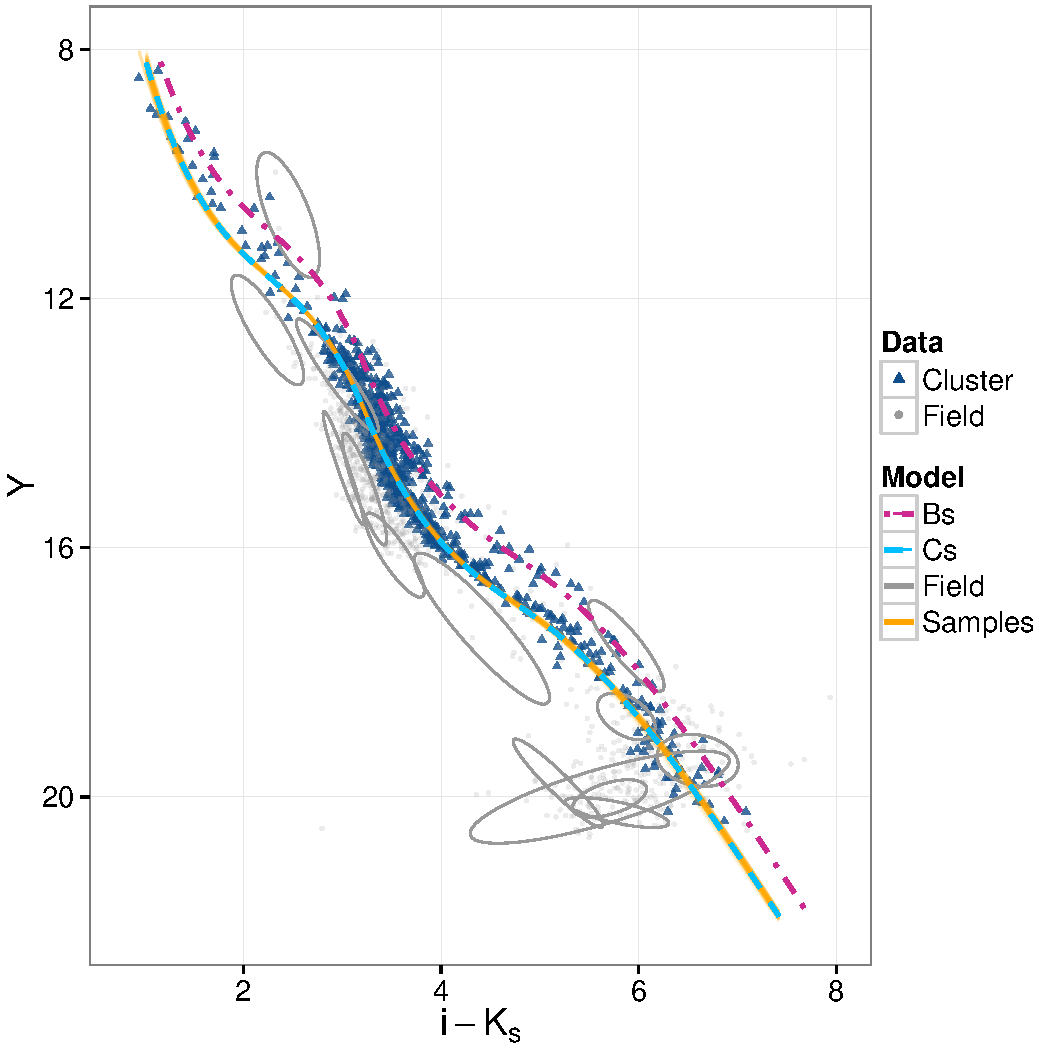
\includegraphics[page=1,height=8cm,width=\textwidth]{background/Figures/BHM/CMDs.pdf}
        \caption{}
    \end{subfigure}
    \begin{subfigure}[t]{0.48\textwidth}
      \includegraphics[page=2,height=8cm,width=\textwidth]{background/Figures/BHM/CMDs.pdf}
        \caption{}
    \end{subfigure}
     \begin{subfigure}[t]{0.48\textwidth}
      \includegraphics[page=3,height=8cm,width=\textwidth]{background/Figures/BHM/CMDs.pdf}
        \caption{}   
    \end{subfigure}
     \begin{subfigure}[t]{0.48\textwidth}
      \includegraphics[page=4,height=8cm,width=\textwidth]{background/Figures/BHM/CMDs.pdf}
        \caption{}
    \end{subfigure}
\caption{\glspl{cmd} showing the cluster and field members (blue triangles and grey dots, respectively resulting from classification using the $p_t = 0.84$ derived in Sect. \ref{sect:classifier}), together with 100 samples (orange spaghetti graphs) from the posterior distributions of the coefficients of the \glspl{bspline} resulting in the \emph{true} values of the cluster photometry. Also shown, the mode of these 100 samples (blue dashed line), the \gls{emb} sequence (magenta dot dashed line) and projections of the photometric field model (grey ellipses).}
\label{fig:CMDs_results}
\end{figure}

\begin{figure}[ht!]
    \centering
      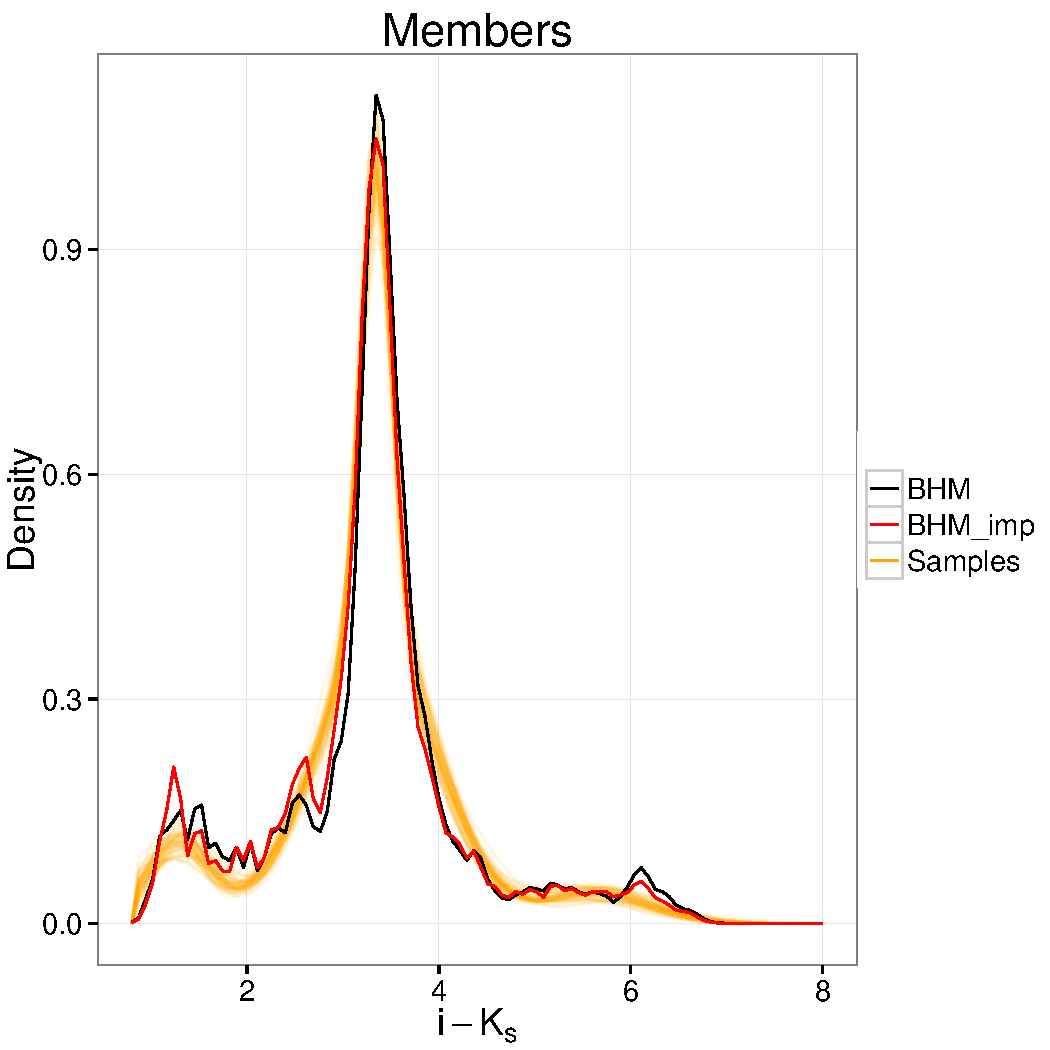
\includegraphics[page=1,width=\textwidth]{background/Figures/BHM/Color_members.pdf}
\caption{\gls{kde} (Gaussian kernel with bandwidth equal to observed uncertainty) of the observed \glspl{ci} of the candidate members of the \gls{bhm} (black line) together with 100 samples from the posterior distribution of the parameters in the \emph{true} \gls{ci} distribution (orange lines). Also shown, the distribution of all \gls{bhm} candidate members (red line, objects with a missing \gls{ci} were imputed from the closest euclidean neighbour).}
\label{fig:CI_results}
\end{figure}



Also, for the sake of completeness, in Fig. \ref{fig:correlations}, I depict the values the correlation coefficients among the 85 parameters in the \gls{bhm}. As can be seen from this Figure, the larger correlations appear among parameters describing the true $\gls{ci}$ distribution, and  among these and almost the rest of the parameters. This is expected since the true $\gls{ci}$ is key parameter in the \gls{bhm}. It is also interesting to notice that there is a strong correlation among the coefficients of the splines series modelling different magnitudes. For example, there is a strong correlation among the fourth coefficients of the splines. These correlations are expected since the shape of the cluster sequence is similar in the four \glspl{cmd}.  

\input{background/Tables/TableParameters.txt}

\begin{figure}[ht!]
\begin{center}
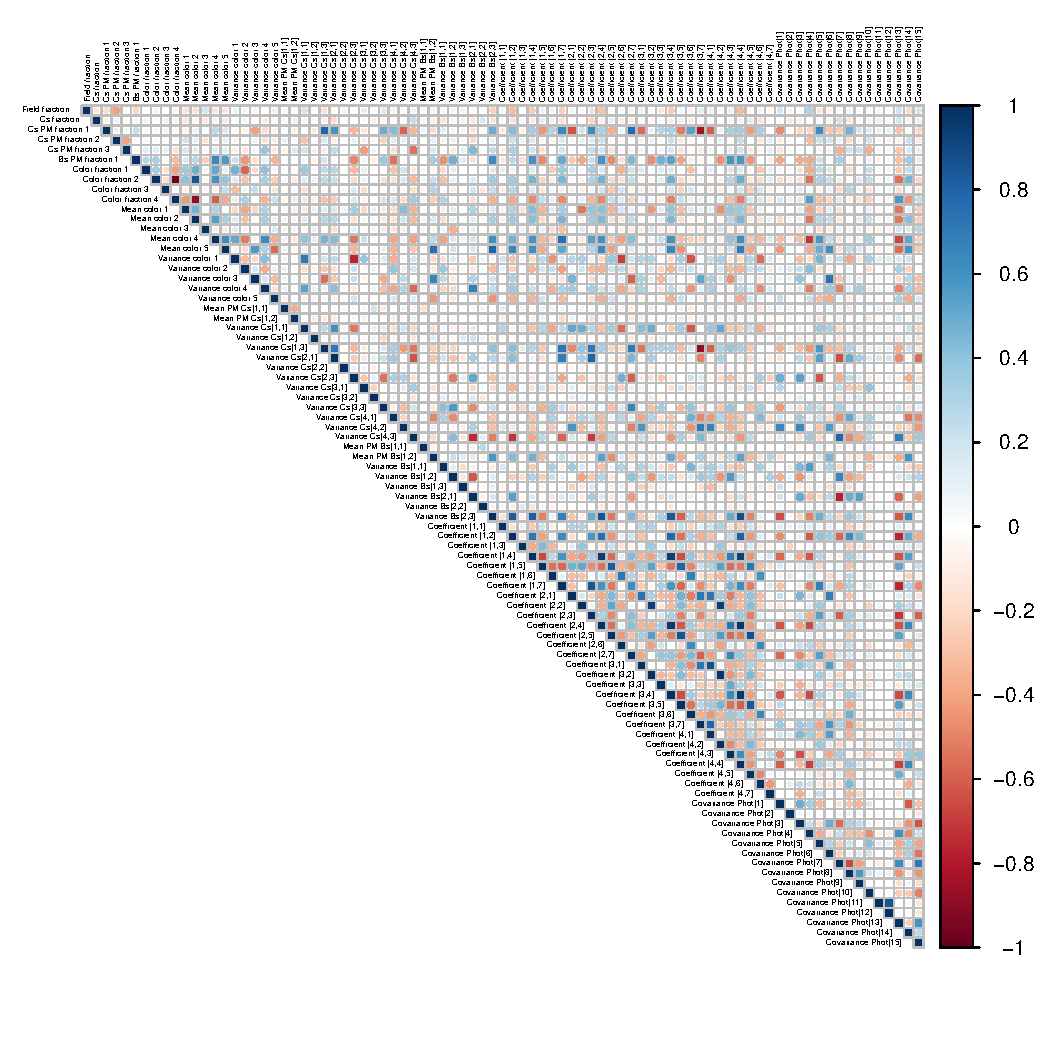
\includegraphics[page=1,width=1.1\textwidth]{background/Figures/BHM/Correlations.pdf}
\caption{Correlation matrix of the posterior distributions of the parameters in the \gls{bhm}. The colour code indicates the value of the correlation coefficient. Parameter names are the same as those in Table \ref{tab:parameters}.}
\label{fig:correlations}
\end{center}
\end{figure}

\section{Updating the prior knowledge}
\label{sect:updating_priors}
As mentioned by \citet{Gelman2006}, the posterior distribution must be inspected to update our previous knowledge. To inspect these posterior distribution, I use the statistics reported in Table \ref{tab:parameters}. These values indicate, for example, that the number of  \gls{gmm} modelling the proper motions of the single stars is overestimated. The fraction and variance of the last gaussian are both to near zero values. Probably, a better model would be that in which the parameters of these extra gaussian will not be part of the model. Ideally, I should choose between these two models based on the evidence they show (see Section \ref{sect:modelselection}). To my knowledge, the only reliable approach to compute the evidence of a model inferred using \gls{mcmc}, is by means of Nested Sampling (see Section \ref{sect:NestedSampling}). However, running the \gls{bhm} in the \emph{MultiNest} package lies beyond our current computational resources.

Another example of inspection of the posterior is the following. In a past run of the \gls{bhm} on the \gls{rdr2}, I realised that the prior distribution for the parameter modelling field fraction was too narrow. Although the maximum of the posterior distribution was allowed by this prior (by definition), the prior density at this \gls{map} was negligible. Therefore, I updated the prior distribution to a distribution with a larger variance. Thus, I weaken the prior information.

\section{Projected spatial distribution}
\label{sect:PSDresults}
In this Section, I present the results of the model selection analysis of the \glsfirst{psd} models of the Pleiades cluster. The Bayesian model selection approach and the \gls{psd} models are described in Sections \ref{sect:modelselection} and \ref{sect:PSDmethod}, respectively. The Bayesian \emph{evidence} is computed with uniform priors for all parameters using the Python package \emph{PyMultiNest} \citep{Buchner2014}. It is a Python wrapper of the C++ package \emph{MultiNest} \citep{Feroz2009} that implements the Nested Sampling algorithm of \citet{Skilling2004,Skilling2006} (see Section \ref{sect:NestedSampling}).

In the Bayesian model selection methodology, the boundaries for decision making from Bayes Factors should be set \emph{ab initio}. Thus, we discuss our results following the classical scale by \cite{Jeffreys61}, which I show in Table \ref{tab:JeffreysScale}.

\begin{table}[H]
\caption{\citet{Jeffreys61} scale for Bayes factors.}
\begin{center}
\begin{tabular}{cc}
Bayes factor & Strength of evidence\\
\hline
0 to 5 & barely worth mentioning\\
5 to 10 & substantial\\
10 to 15 & strong\\
15 to 20 & very strong\\
$>$ 20 & decisive\\
\hline
\end{tabular}
\end{center}
\label{tab:JeffreysScale}
\end{table}%
 


\subsection{Selection of models with radial symmetry} 

Tables \ref{tab:BayesFactors3deg} and \ref{tab:BayesFactors6deg} summarise the evidences and Bayes factors of the radially symmetric models using the candidate members within  7 pc (3$^{\circ}$) and 14 pc (6$^{\circ}$), respectively. 
\begin{table}[ht]
  \centering
      \caption{Natural logarithm of the evidence (diagonal) and Bayes factors (off-diagonal elements) for each radially symmetric model inferred from the 7 pc (3$^\circ$) sample.}
         \begin{tabular}{rcccccc}
           & King & OGKing  &   GKing & EFF & GP & RGP \\
\hline              
           King    &-2876.2 &  0.13   &   0.04  &  0.03   &   0.04  &  0.41  \\
           OGKing  &   7.39     &-2878.2  &   0.33  &  0.25   &   0.3   &  3.00  \\
           GKing   &    22.19    &    3.0     &-2879.3  &  0.74   &   0.90  &  9.02  \\
           EFF     &    29.96    &      4.0   &   1.34      &-2879.6  &   1.22  & 12.18  \\
           GP      &    24.53    &     3.32    &   1.1      &    0.81     &-2879.4  &  9.97  \\
           RGP     &   2.45     &     0.33    &    0.14     &      0.08   &   0.1      &-2877.1 \\
           \hline
\multicolumn{7}{l}{
  \begin{minipage}{12cm}
    {\footnotesize Note. Bayes factors are computed with evidence of the model specified in the column header placed in the numerator and in the row header in the denominator.}
  \end{minipage}
}
\end{tabular}
        
  \label{tab:BayesFactors3deg}
   \end{table}
   
\begin{table}[ht]
  \centering 
 \caption[]{Natural logarithm of the evidence (diagonal) and Bayes factors (off-diagonal elements, computed as in Table \ref{tab:BayesFactors3deg}) for each profile radially symmetric model inferred from the 14 pc (6$^{\circ}$) sample.}

\begin{tabular}{rcccccc} 
&King & OGKing & GKing & EFF & GP & RGP \\
\hline              
           King    &-5033.5       &  $>100$  &   2.7    &   $<0.01$     &  3.3       &    27.113  \\
           OGKing  &    $<0.1$&  -5023.6 &  $<0.01$ &   $<0.01$     &   $<0.01$  &   $<0.01$   \\
           GKing   &    0.36     &  $>100$   & -5032.5  &   $<0.01$     &  1.2       &   10.0     \\
           EFF     &    $>100$ & $>100$ &    $>100$  &   -5044.1     &  $>100$    &   $>100$   \\
           GP      &   0.3          &   $>100$ &    0.81      &    $<0.01$    &   -5032.3    & 8.2      \\
           RGP     &   0.03      &   $>100$  &    0.1      &     $<0.01$    &   0.12           & -5030.2     \\
         \end{tabular}
 
 \label{tab:BayesFactors6deg}
   \end{table}
  


We primarily focus on the 7 pc (3$^{\circ}$) sample, where the completeness and depth are most homogeneous (see Section \ref{sect:DR2}). As can be seen in Table \ref{tab:BayesFactors3deg}, the Bayes Factors are in the ranges between 1 and 3 (differences \emph{barely worth mentioning} in Jeffrey's scale) and between 3 and 10 (\emph{substantial evidence}).

The King's and the \gls{rgp} models have the largest evidences and a Bayes Factor of 0.41 (or 2.43) between them. It implies that there is no reason to prefer one over the other. According to Jeffrey's scale, this difference \emph{barely worth mentioning}. At the same time, King's model, the one with the highest evidence, shows Bayes Factors in the category between 3 and $\sim$10 (\emph{substantial evidence}) or even up to 30 (\emph{strong evidence}) when compared to the remaining models (\gls{ogking}, \gls{gking}, \gls{eff} and \gls{gp}).  

In Figure \ref{fig:King_7}, we show the projections of the posterior distribution for King's model parameters inferred from the 7 pc (3$^{\circ}$) sample. As can be seen, the tidal radius is relatively unconstrained by the data. This can be understood in terms of the lack of observations in the vicinity of the cluster edge (tidal radius), which introduces a degeneracy. The maximum a posteriori (\gls{map}) values of the parameters of King's profile are $\alpha_c=56.65496^{\circ}$, $\delta_c=24.13461^{\circ}$, $r_c=2.0$ pc and $r_t=44.7$pc. We also fit a multivariate Gaussian to the posterior distribution at the \gls{map} estimate, it yields the following standard deviation matrix:

$$
\left(\begin{array}{rrrr}
 0.000045   & -0.000004  &  0.000205  & -0.0008  \\
-0.000004   &  0.000038  & -0.000005  & -0.0002  \\
 0.000205   & -0.000005  &  0.20      & -0.3646  \\
-0.000805   & -0.000233  & -0.364647  &  28.048  \\
\end{array}\right)
$$
with the above ordering of parameters ($\alpha_c, \delta_c, r_c$, and $r_t$). 

\begin{figure}[htbp]
\begin{center}
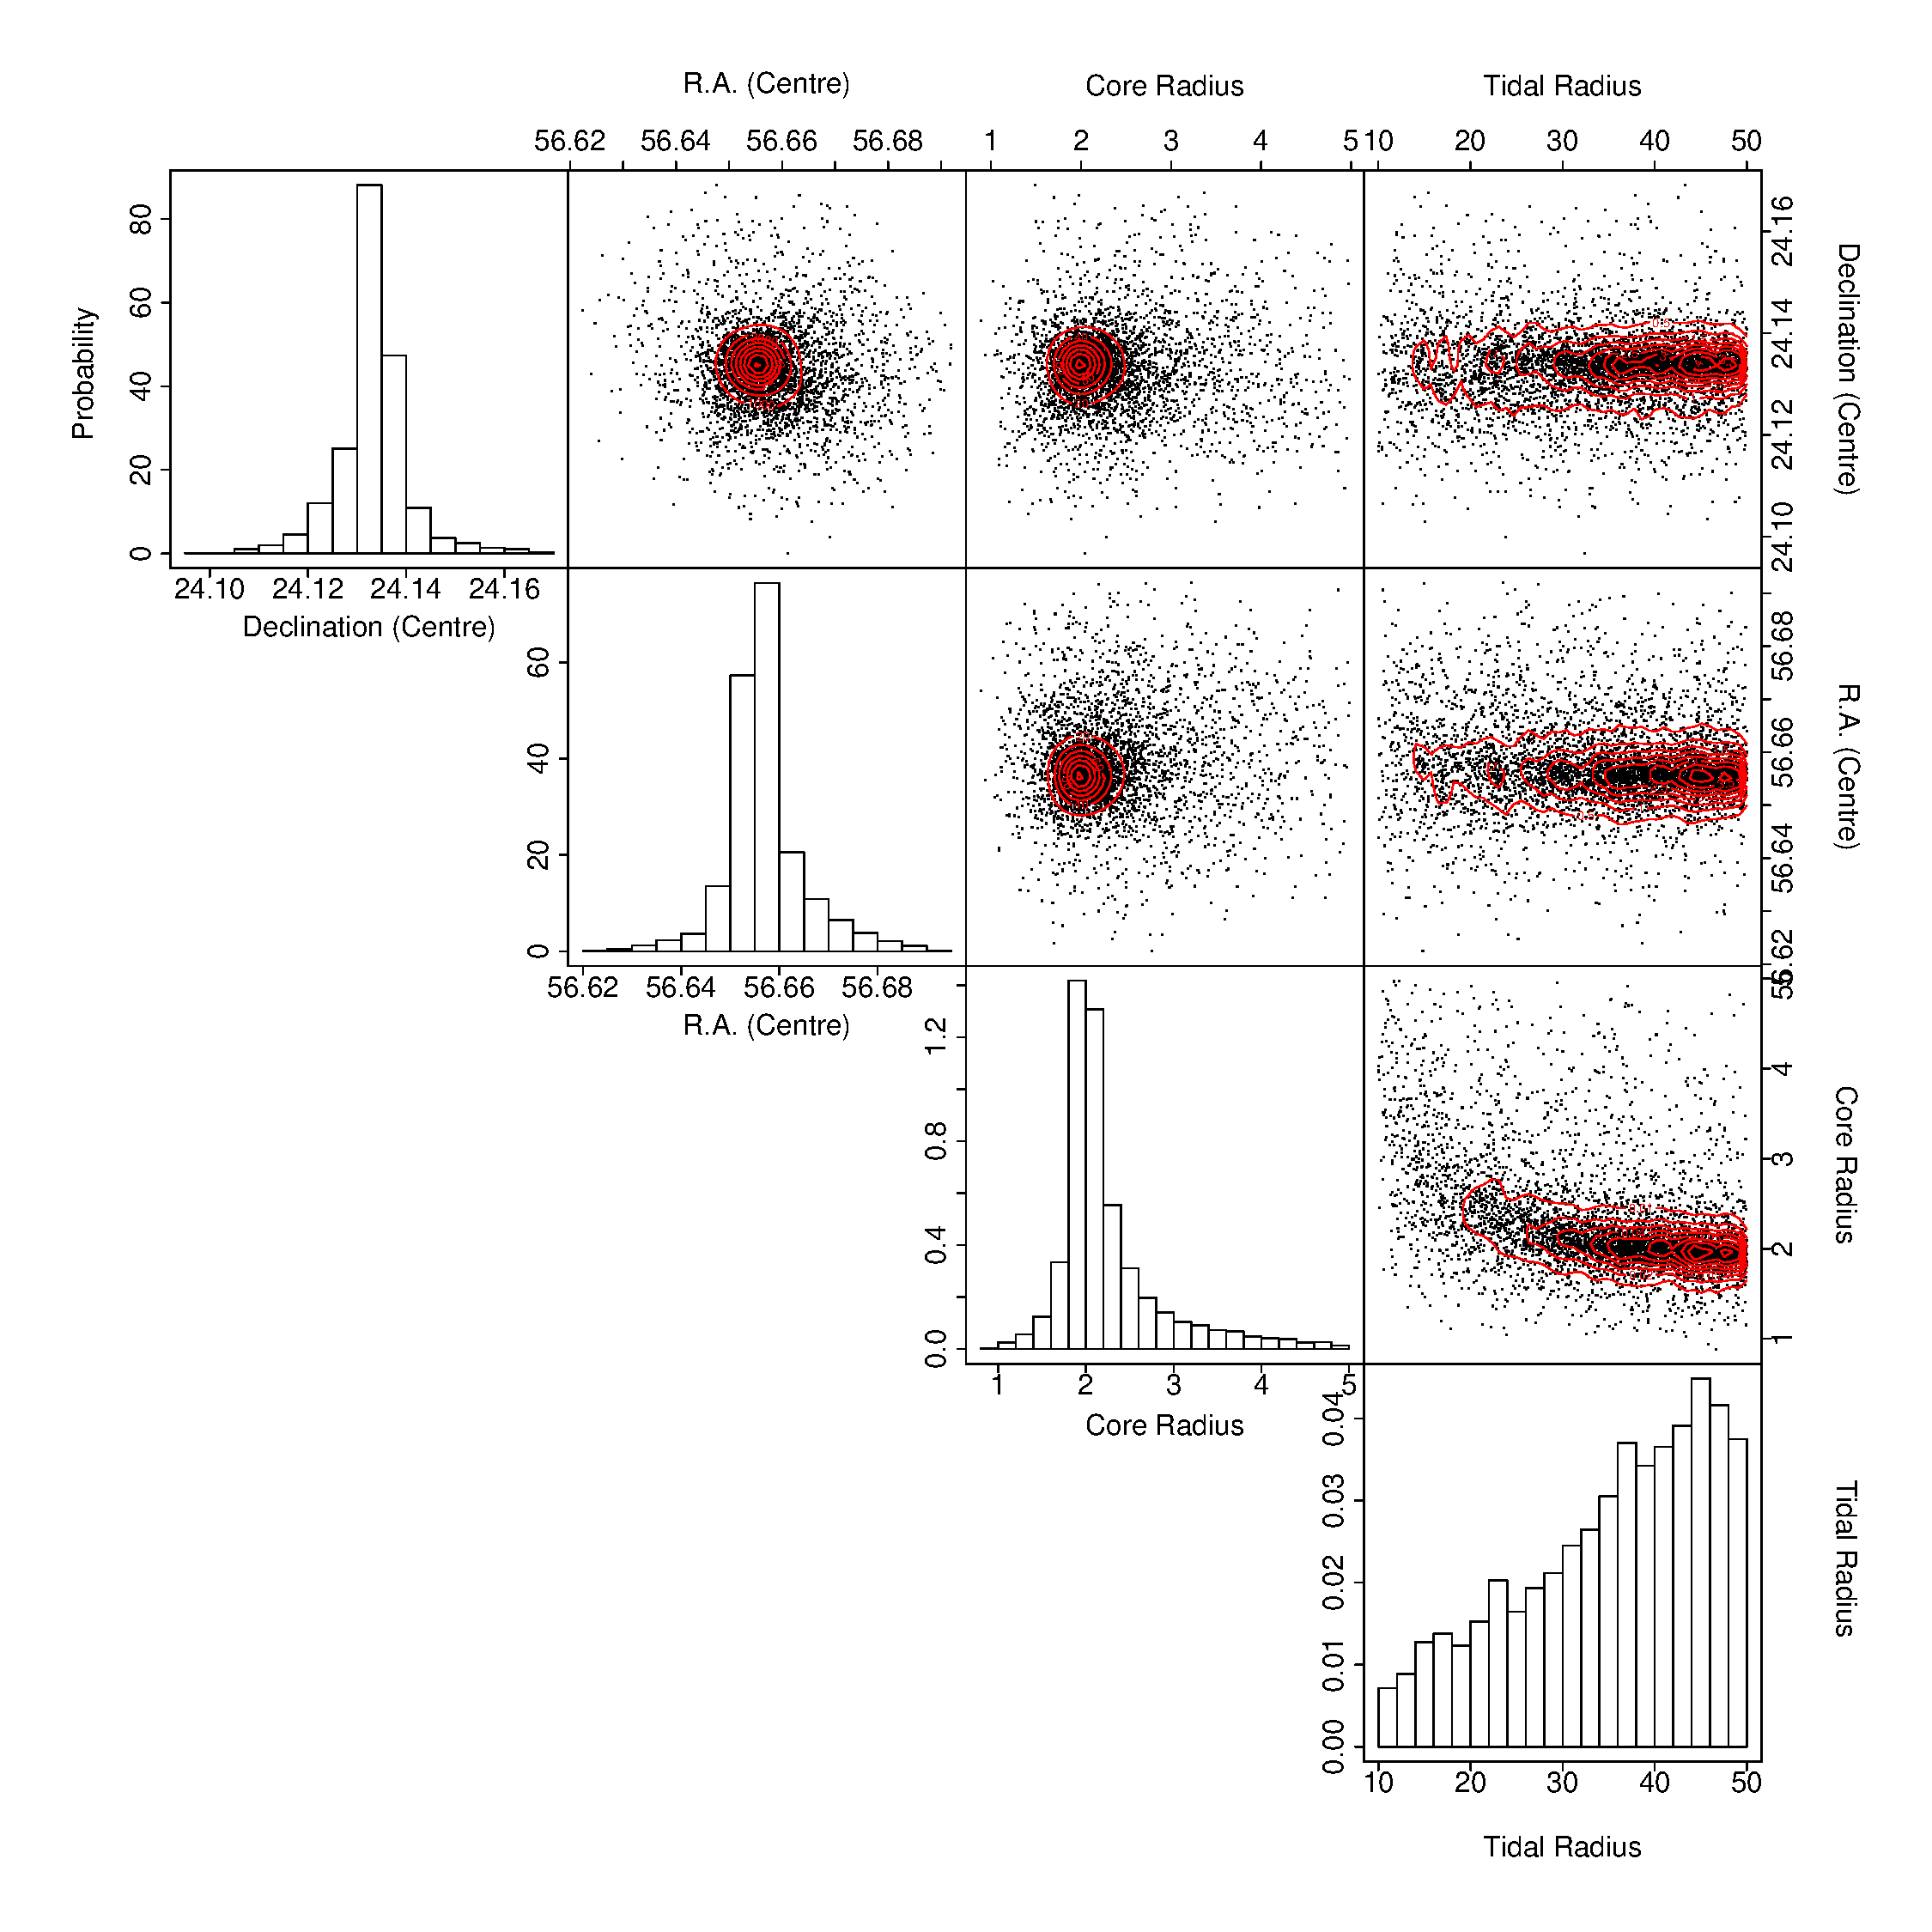
\includegraphics[width=\textwidth]{background/Figures/PSD/King7.pdf}
\caption{Samples of the posterior distribution of the King's profile parameters inferred from the 3$^{\circ}$. The core and tidal radius are in pc. }
\label{fig:King_7}
\end{center}
\end{figure}


We will first compare King's model with the \gls{gking} profile. \gls{gking} is a model with significantly less evidence and two more parameters than King's profile. The posterior distributions reveal a complete loss of interpretability of the parameters, with the core radius relatively unconstrained between 100 and 400 pc, tidal radii between 200 and 800. %The $a$ exponent is the only well constrained parameter (\gls{map} value of XXXX)

The second alternative is the modified King profile with exponents fixed to the maximum evidence values (\gls{ogking}). In this case, the model has the same number of parameters as in the classical King profile, but we have selected the values of $\alpha_1$ and $\alpha_2$ in Eq. \ref{eq:GKing} that maximise the evidence (0.4 and 1.2 respectively, compared to 0.5 and 2 in the classical King profile). It is important to bear in mind that the maximum evidence is attained for the 6$^{\circ}$ sample, and this evidence is no longer maximum when calculated with the 3$^{\circ}$ sample. In this case, the parameters retain the interpretability (for obvious reasons) and the tidal radius is relatively well constrained ($\pm 7$pc). However, the evidence is reduced with respect to the classical King profile despite the increased maximum likelihood. We interpret this as the result of overfitting in the process of fixing the $a$ and $b$ parameters. The \gls{map} estimates of the \gls{ogking} profile parameters are $\alpha_c=56.65603^{\circ}$, $\delta_c=24.13292^{\circ}$, $r_c=1.15$ pc and $r_t=13$ pc. The standard deviation matrix of the multivariate normal fitted at the \gls{map} is 

$$
\left(\begin{array}{rrrr}
 0.000028 &-0.000003 & 0.000009 & 0.00063\\
-0.000003 & 0.000026 & 0.000039 &-0.00007\\
 0.000009 & 0.000039 & 0.149843 &-0.28731\\
 0.000627 &-0.000070 &-0.287310 & 6.69046\\
\end{array}\right).
$$


The two profiles (King and \gls{ogking}) are relatively similar despite the different exponents and \gls{map} parameter estimates. 

Finally (we will not discuss the \gls{eff} or \gls{gp} profiles), the \gls{rgp} suffers the same loss of interpretability encountered for the \gls{gking} profile, with an unconstrained core radius in the range of hundreds of parsecs. Also the posterior distributions of the $R_b$ and $b$ parameters are unconstrained, with a large correlation between $a$ and $b$. The resulting density profile is also cusped at the centre of the cluster. 

%\begin{figure}[ht!]
%\begin{center}
%%\includegraphics[width=\textwidth]{background/Figures/PSD/GKing7.pdf}
%\caption{Posterior distributions of the parameters in the GKing profile. }
%\label{fig:GKing7}
%\end{center}
%\end{figure}

As a summary of the results of the 3$^{\circ}$ sample, we find that the introduction of more flexibility in the analytical expressions of the classical radially symmetric profiles does not produce larger evidences, and results in some cases in unconstrained parameters and a loss of the interpretability associated to the original formulations. Therefore, for the data set that extends out to 3$^{\circ}$ there are two competing models (classical King and \gls{rgp}) and there is no sufficient evidence to select amongst them. The central part is reasonably well fitted either by a King's profile with relatively well constrained parameters or with a \gls{rgp} profile with large degeneracy.  Only additional, perfectly acceptable prejudices like physical interpretability or the ability to compare with previous results, can be invoked to choose the King's profile over the rest.


Concerning the 6$^{\circ}$ sample, the \gls{ogking} profile has the largest evidence. It comes as no surprise since \gls{ogking} profile fixes the values of $\alpha_1$ and $\alpha_2$ to those that yield the maximum evidence. Hence, we acknowledge overfitting to the incomplete and biased sample of Pleiades members out to 6$^{\circ}$. In fact, the marginal posterior distribution for the tidal radius is sharply peaked around 16 pc, only slightly further than the observational boundary.

For the \gls{rgp} model, its \gls{map} estimates are $\alpha_c=56.6909785^{\circ}$, $\delta_c=24.13301438^{\circ}$, $R_b=886.84$ pc , $\alpha=1.44$, and $\beta=70.6$. The corresponding standard deviation matrix is

$$
\left(\begin{array}{rrrrr}
 0.0000589  & 0.000006 &   -0.02 &-0.0000001 &  -0.003  \\
 0.0000061 & 0.000049 &    0.01 & 0.0000134 &  -0.002\\
-0.0243964 & 0.011738 &20173.20 & 3.0774488 & 616.625\\
-0.0000001 & 0.000013 &    3.08 & 0.0219039 &  -2.316\\
-0.0028333 &-0.002123 &  616.63 &-2.3162244 & 331.945\\
\end{array}\right).
$$

It is evident from the previous matrix that $R_b$ and $\beta$ are only mildly constrained. The profile is, again, characterised by a cusp in the central part of the cluster, as is the profile of the \gls{gking} alternative. 

The 6$^{\circ}$ data set favours  \gls{map} profiles (models and \gls{map} estimates of their parameters) with sharp peaks in the centre of the cluster. However, we caution the reader against these results. They refer to a data set that is severely biased and incomplete in ways that we cannot quantify and/or model.

The conclusion from the comparison of these radially symmetric profiles in the context of the two data sets is that i) there is no compelling reason to abandon the widely used King profile in the context of the complete and homogeneous data set out to 3$^{\circ}$ and ii) there are better models when evaluated on data out to 6$^{\circ}$, but it remains to be found whether this is due to the completeness problems of the \gls{dance} data in the outer regions of the Pleiades or whether they truly represent a need to make the King profile more flexible to accommodate the data. In the following we retain three of the models discussed above (King, \gls{ogking} and \gls{rgp}), and take the comparison one step further in order to accommodate simple deviations from radial symmetry in the form of elliptical density contours.

\subsection{Selection of models with biaxial symmetry}

Concerning the models with biaxial symmetry, Table \ref{tab:BayesFactorsEll} collects the evidences and Bayes factors. We have included the results for the \gls{ogking} alternative despite the fact that we had to extend the support of the prior for the $r_{t,a}$ and $r_{t,b}$ parameters out to 300 pc. For smaller values of the support, the \gls{mcmc} samples possess maxima at the boundaries. Even in the set up with priors extending out to 300 pc, the parameter samples lack physical interpretations with vanishingly small \gls{map} core radii. We see that the \gls{ogking} profile is clearly to be preferred when compared against the other two models, and any of the three is to be preferred to the radially symmetric profiles of Table \ref{tab:BayesFactorsEll}. However, despite the fact that the \gls{ogking} shows the best evidence and the largest Bayes factor, the unconstrained and unphysical values of its parameters allow us to discard it, and continue exploring the luminosity segregation only in the King model.

\begin{table}[ht!]
  \centering
  \caption[]{Natural logarithm of the evidences (diagonal) and Bayes factors (off-diagonal, computed as  in Table \ref{tab:BayesFactors3deg}) for the models with biaxial symmetry inferred from the $3^{\circ}$ and $6^{\circ}$ samples. }
  \label{tab:BayesFactorsEll}

\begin{tabular}{cl|ccc|ccc|}
\hline              
\hline              
&&  \multicolumn{3}{c}{$3^{\circ}$} &   \multicolumn{3}{c}{$6^{\circ}$} \\
\hline              
&&  King & OGKing & RGP &  King &  OGKing & RGP \\
\hline              
\multirow{3}{*}{$3^{\circ}$}           &King    &  -2806.9   &  $>100$   &    0.14   &           &            &               \\
           &OGKing  &            &   -1527.3 & $<0.01$   &           &            &               \\   
           &RGP     &            &           &  -2808.9  &           &            &               \\
           \hline
\multirow{3}{*}{$6^{\circ}$}          &King    &            &           &           &  -5023.8  &  $>100$    &   $<0.01$     \\
           &OGKing  &            &           &           &           &  -3255.7   &   $<0.01$     \\   
           &RGP     &            &           &           &           &            &  -5034.7      \\
\hline              
         \end{tabular}
   \end{table}

\begin{figure}[ht!]
 \centering
  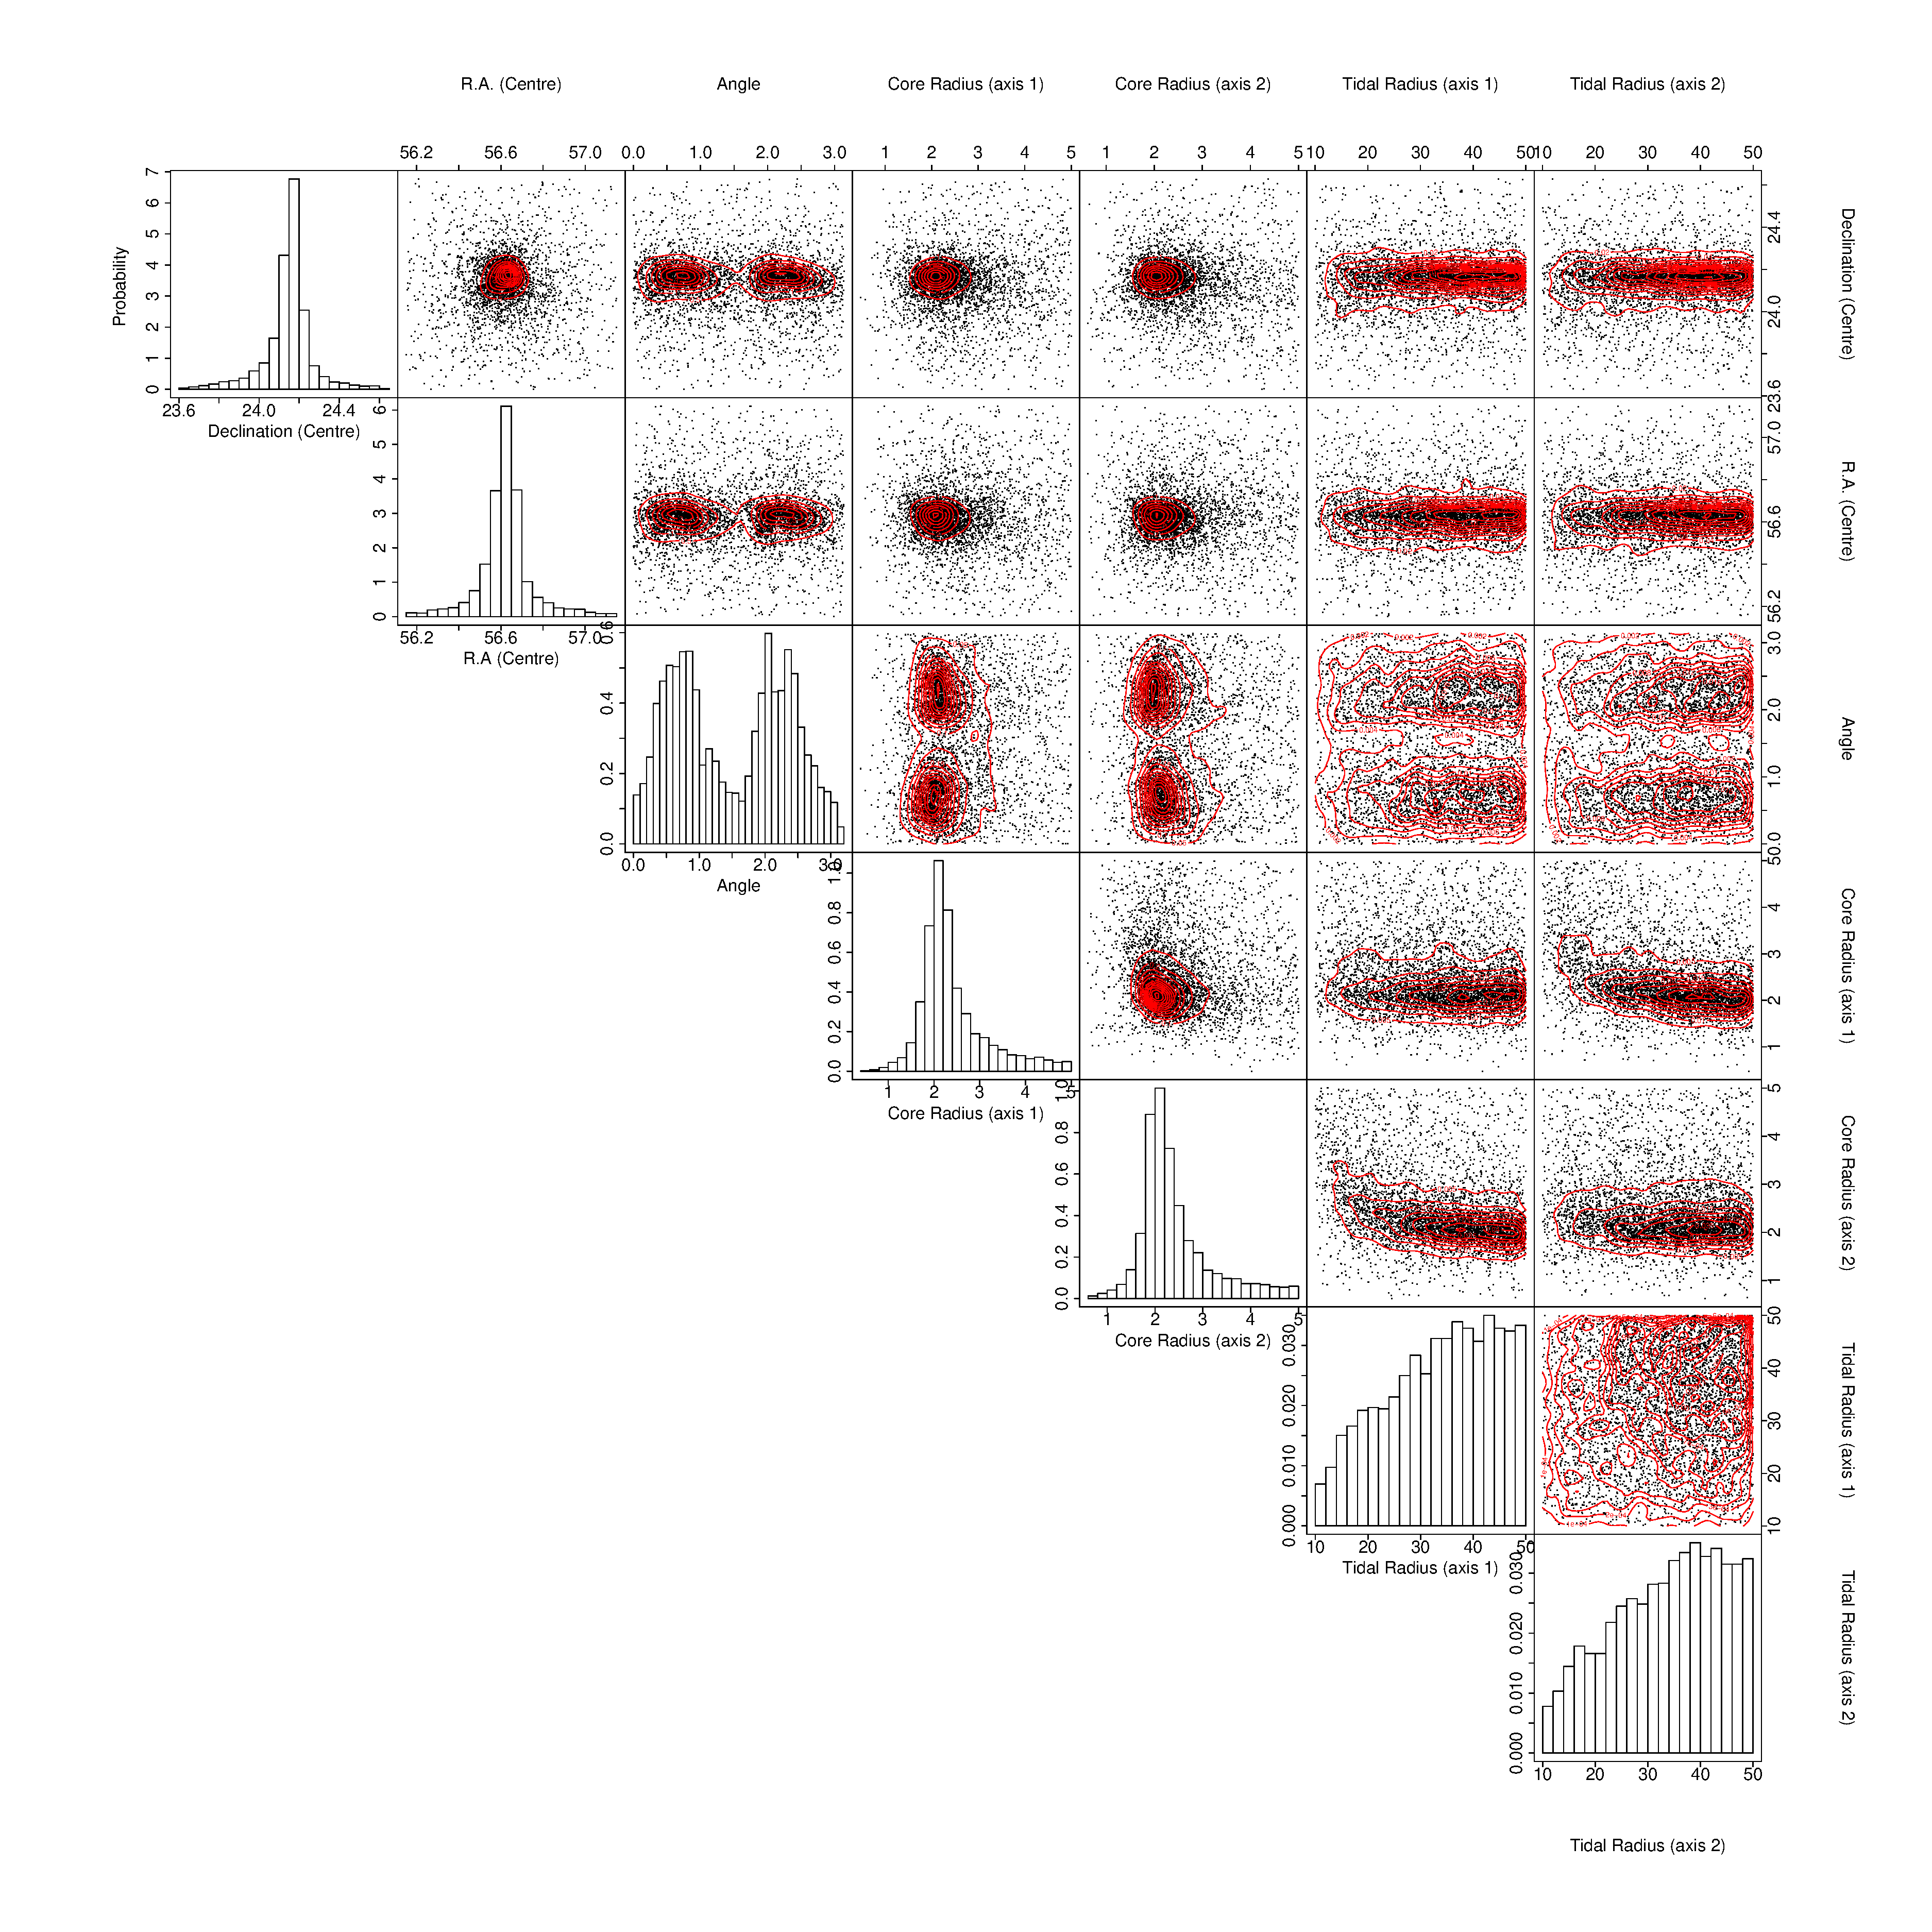
\includegraphics[width=\textwidth]{background/Figures/PSD/KingEll7.pdf}
  \caption{Samples from the posterior distribution of the parameters in the biaxial symmetric King model inferred from the 3$^{\circ}$ sample. Tidal and core radius are in units of pc.}
\label{fig:KingEll7}
\end {figure}

The \gls{map} estimates of the King model on the $3^{\circ}$ sample are $\alpha_c=56.66025602372^{\circ}$ , $\delta_c=24.2038 ^{\circ}$, $\phi=2.1$ rad, $r_{cx}=1.84$ pc, $r_{cy}=$1.77 pc ,$r_{tx}=$ 48.9 pc, and $r_{ty}=$48.5 pc. The standard deviation matrix is

$$
\tiny
\left(\begin{array}{rrrrrrr}
 0.0124 & 0.0003 & 0.0004 &-0.0004 & 0.0002 & -0.0006 &  0.011\\
 0.0003 & 0.0111 &-0.0025 &-0.0069 & 0.0002 & -0.0065 &  0.008\\
 0.0004 &-0.0025 & 0.7070 &-0.0377 & 0.0540 &  0.2696 & -0.013\\
-0.0004 &-0.0069 &-0.0377 & 0.3749 &-0.0244 & -0.0387 & -0.703\\
 0.0002 & 0.0002 & 0.0540 &-0.0244 & 0.3722 & -0.9000 &  0.017\\
-0.0006 &-0.0065 & 0.2696 &-0.0387 &-0.9000 & 59.3446 &-12.580\\
 0.0113 & 0.0076 &-0.0129 &-0.7034 & 0.0174 &-12.5795 & 60.462\\
\end{array}\right)
$$
with the ordering of parameters used above.

Interestingly, this \gls{map} shows no evidence of ellipticity\footnote{The ellipticity is defined as $\epsilon = 1 - \frac{b}{a}$, with $a$ and $b$ the semi-major and semi-minor axis of the ellipse, respectively.} neither in the core radius ($\epsilon_{rc}= 0.04$) nor in the tidal radius ($\epsilon_{rt}= 0.008$). Despite this fact, the biaxial symmetric King models have decisive evidence when compared to the radially symmetric ones (see Table \ref{tab:BayesFactorsAll}).

\subsection{Selection of models with luminosity segregation}
\label{sect:lumsegregation}
In this Section, I describe the luminosity ($J$ band) segregation (see Section \ref{sect:SegregatedModels}) included only in the radial and biaxial symmetric extensions of the King profile. As shown in the previous section, King's profile not just has large Bayes factor, but also physical interpretability. Table \ref{tab:BayesFactorsLumSeg} summarises the evidences and Bayes Factors of the \gls{krs} and \gls{kbs}. The parameters of these models and its evidences are inferred using  the  3$^\circ$ and 6$^\circ$ samples.

\begin{table}[ht!]
  \centering
  \caption[]{Natural logarithm of the evidences (diagonal) and Bayes factors (off-diagonal, computed as in Table \ref{tab:BayesFactors3deg}) for the radial and biaxial symmetric models with luminosity segregation inferred from the 3$^\circ$ and 6$^\circ$ samples. }
  \label{tab:BayesFactorsLumSeg}
\begin{tabular}{cc|cc|cc}
\hline              
\hline              
&&  \multicolumn{2}{c}{$3^{\circ}$} &   \multicolumn{2}{c}{$6^{\circ}$} \\
\hline              
& & King-Radial& King-Biaxial &  King-Radial &  King-Biaxial \\
\hline              
\multirow{2}{*}{$3^{\circ}$}&King-Radial    &  -2875.5   &    $>100$       &           &            \\
&King-Biaxial &            &  -2803.9  &           &            \\
\hline
\multirow{2}{*}{$6^{\circ}$}& King-Radial    &            &           &   -5025.4 &    $>100$        \\
&King-Biaxial &&                     &           &  -5016.4   \\
\hline              
         \end{tabular}
   \end{table}

Figures \ref{fig:KingRS7} and \ref{fig:KingBS7} show the posterior distributions of the parameters \gls{krs} and \gls{kbs} models, respectively. Both models are inferred from the complete 3$^{\circ}$ sample. Their \gls{map} values and standard deviation matrices of their parameters are the following. 

The \gls{map} values of the \gls{krs} model are $\alpha_c=56.6264^{\circ}$ , $\delta_c=24.1956^{\circ}$, $r_{c}=2.115$ pc, $r_{t}=$ 31.778 pc, and $\kappa= 0.127\, \rm{pc \cdot mag^{-1}}$. Its standard deviation matrix (with parameters in the same previous order) is

$$
\tiny
\left(\begin{array}{rrrrr}
0.0077725911  & 0.0011463608 & 0.015866753 & -0.006895138 &0.0004781459\\
0.0011463608  & 0.0066805294 & 0.009640874 &  0.011311284  &0.0002655555\\
0.0158667525  & 0.0096408739 & 0.380770948& -0.844035083  & 0.0210177901\\
-0.0068951385 & 0.0113112840 & -0.844035083& 45.371984935&-0.0671929448\\
0.0004781459  & 0.0002655555 & 0.021017790& -0.067192945  &  0.0048742344\\
\end{array}\right)
$$

The \gls{map} values of the \gls{kbs} model are $\alpha_c=56.6006^{\circ}$, $\delta_c=24.193^{\circ}$, $\phi=1.915$ rad, $r_{cx}=2.348$ pc, $r_{cy}=$2.042 pc ,$r_{tx}=$ 38.12 pc, $r_{ty}=$48.382 pc  and $\kappa= 0.147\, \rm{pc \cdot mag^{-1}}$. Its standard deviation matrix (with parameters in the same previous order) is

$$
\tiny
\left(\begin{array}{rrrrrrrr}
0.0139885233 	 &  -0.0002135887  &-0.002818604  & 0.007312077     &0.004963964   &  0.02605645     &-0.003657460      &-0.0001631951\\
-0.0002135887 	 &  0.0130671231   &-0.001734756   & -0.003808827   &-0.001210257  &  0.03990854     &-0.013443550      &0.0006731357     \\        
-0.0028186038 	 & -0.0017347556   & 0.727100779   & 0.013468602    &0.005179071    & -0.55449101    & 0.596346854      &0.0011082365      \\           
0.0073120769 	 &   -0.0038088265 &  0.013468602  &  0.422814580   &0.054674731    & -0.19355524    & -0.679337642     & 0.0107408223     \\  
0.0049639637 	 &   -0.0012102569 &  0.005179071  &  0.054674731   &0.433668247    & -1.66048288    & 0.346810670      & 0.0131324789     \\      
0.0260564469 	 &   0.0399085427  & -0.554491013  &  -0.193555244  & -1.660482881 &  89.94363663   & -13.562539506   & -0.0592770535   \\        
-0.0036574599 	 &  -0.0134435502  &  0.596346854  & -0.679337642   & 0.346810670  &  -13.56253951  &   56.110848655  &  -0.0089581971   \\          
-0.0001631951 	 &   0.0006731357  & 0.001108236   & 0.010740822    & 0.013132479   &   -0.05927705  &    -0.008958197  &   0.0040960558    \\
\end{array}\right)
$$


As can be seen from the \gls{map} values and its standard deviation, the $\kappa$ luminosity segregation parameter is similar and significative for both \gls{krs} and \gls{kbs} models. Concerning the ellipticity, the core radius and tidal radius have large values, $\epsilon_{rc}= 0.13$ and $\epsilon_{rt}= 0.21$, respectively. However, due to the large uncertainties in the tidal radii, we trust only in the ellipticity reported for the core radius. The latter value is nevertheless similar to those previously reported in the literature \cite[0.17 and 0.1 to 0.35 reported by][respectively]{Raboud1998,Adams2001}. We do not report the ellipticity value inferred from the extended 6$^\circ$ sample due to the incompleteness of the latter. Indeed, this ellipticity can be strongly biased by the patchy pattern of the \gls{ddr2} observations.

\begin{figure}[ht!]
 \centering
  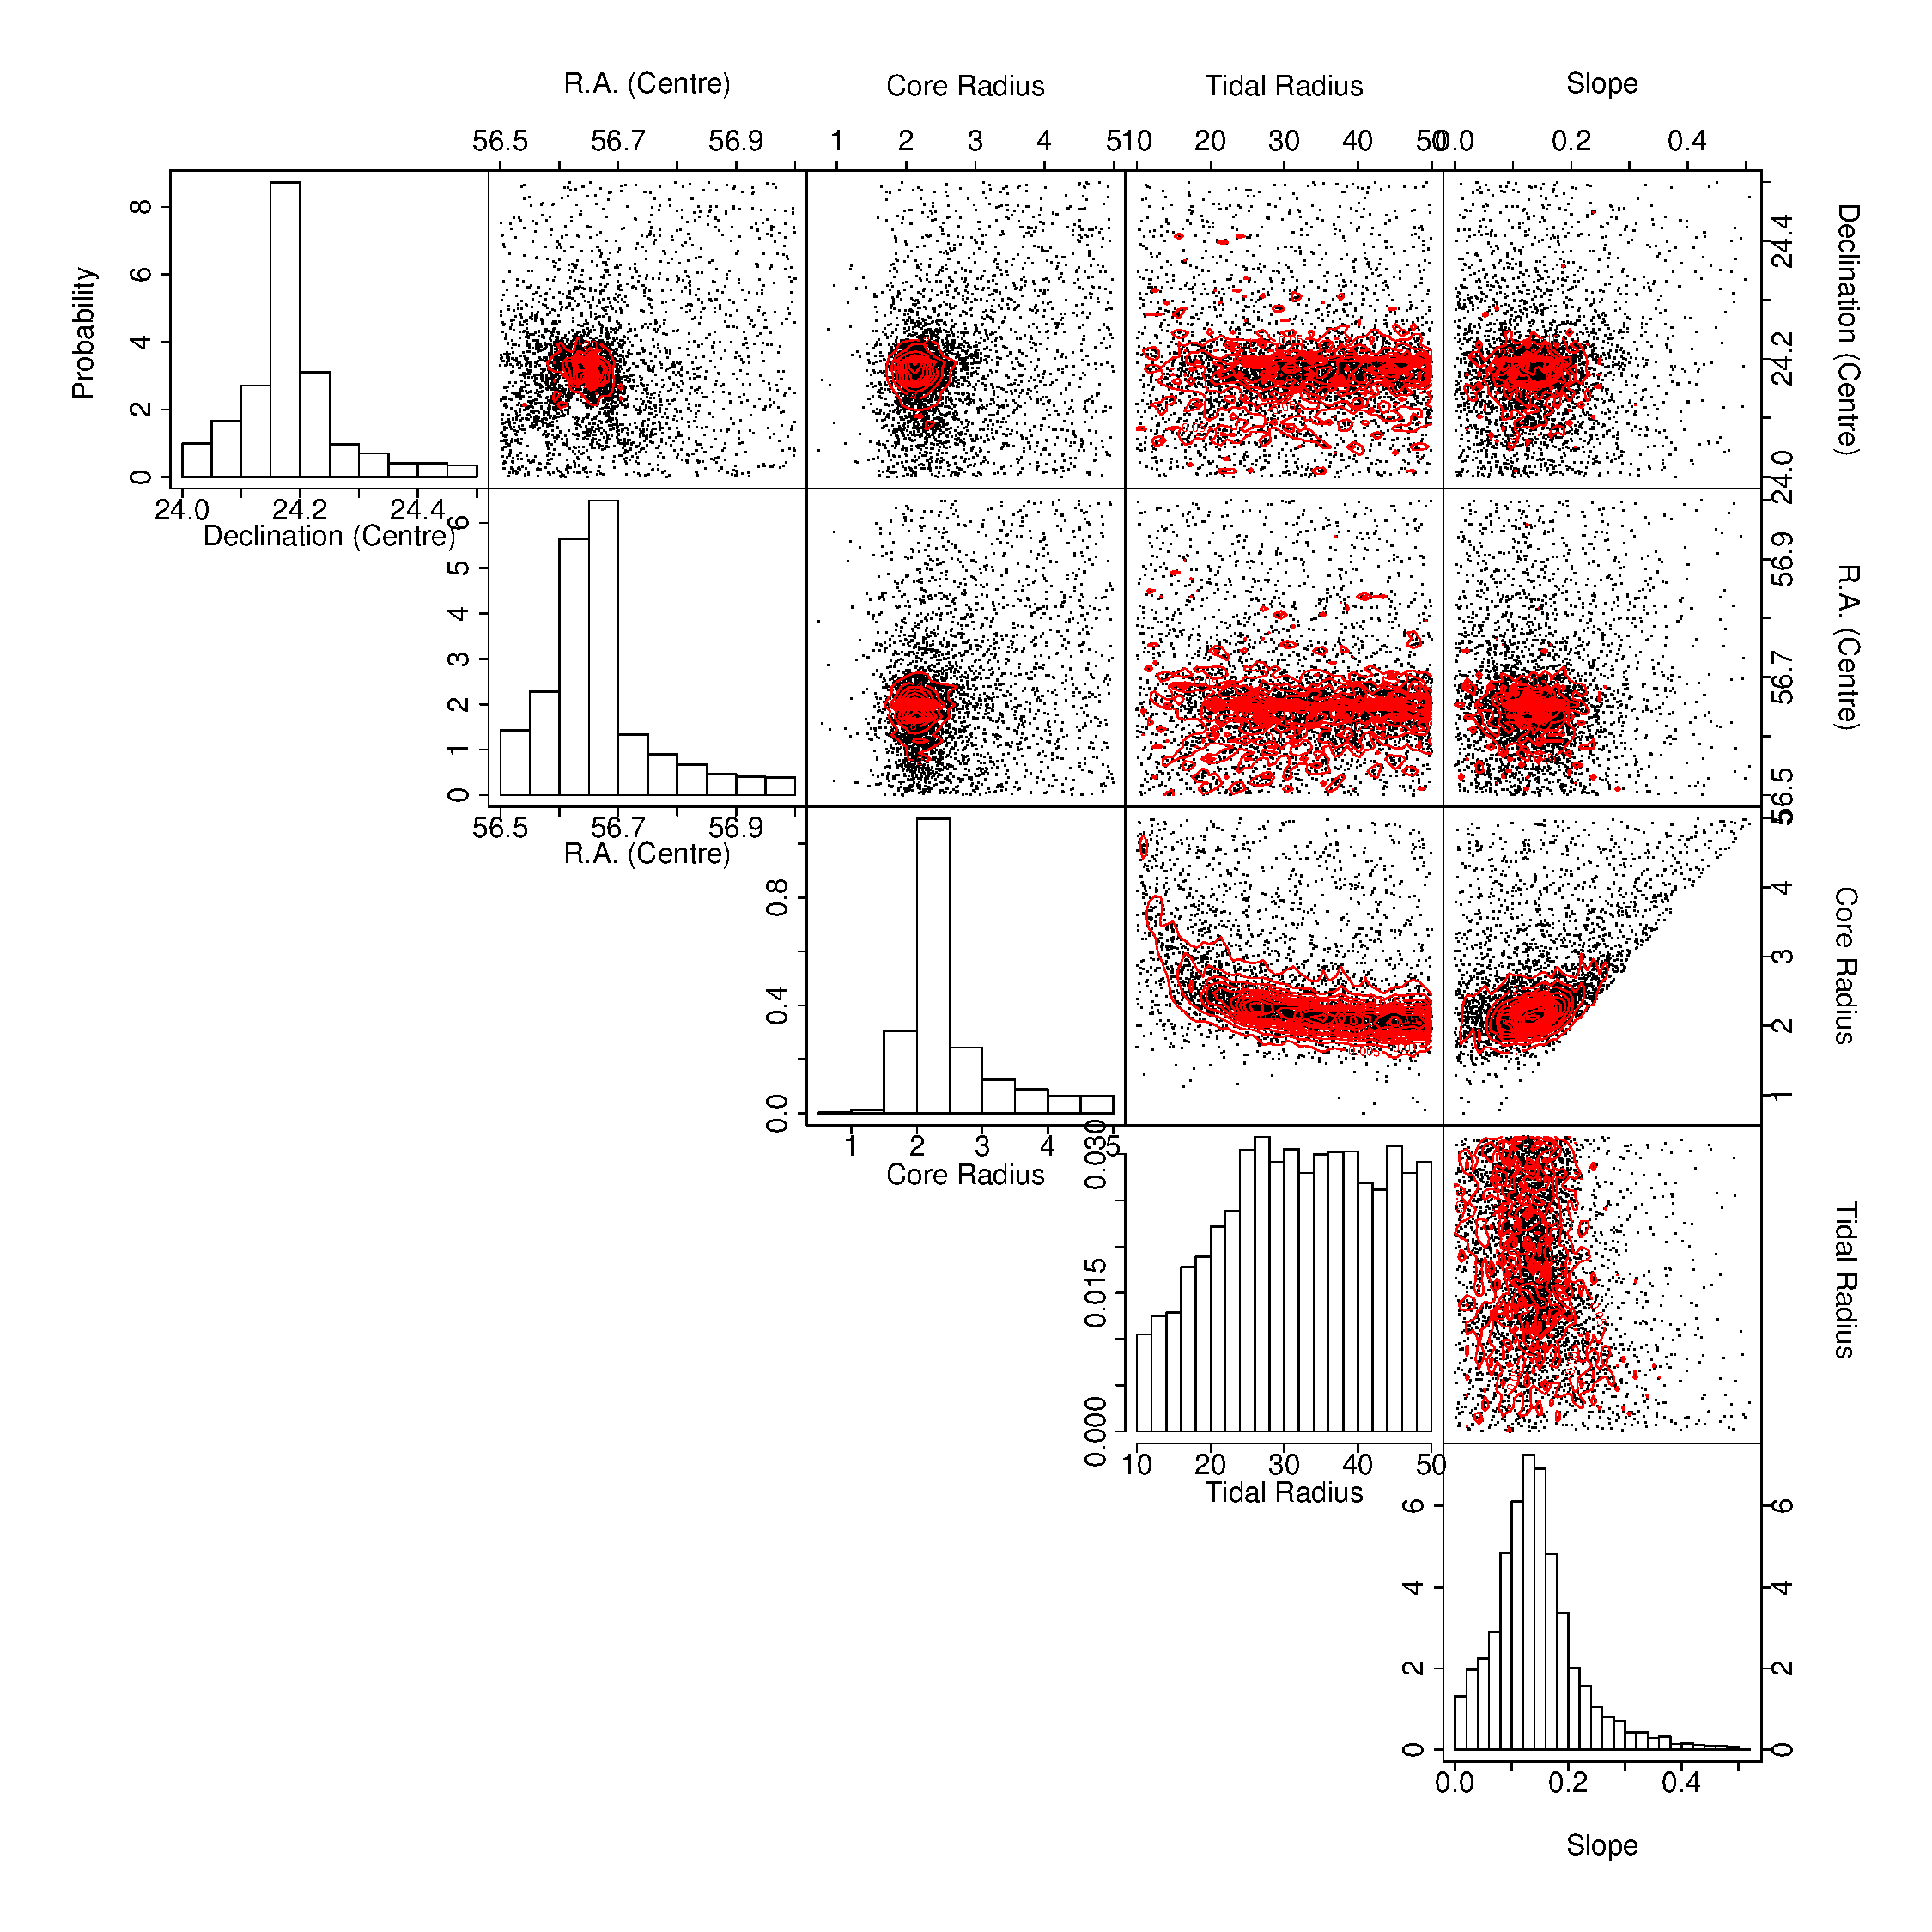
\includegraphics[width=\textwidth]{background/Figures/PSD/KingRS7.pdf}
  \caption{Samples of the posterior distribution of the parameters in the radially symmetric and luminosity segregated King model inferred from the 3$^{\circ}$ sample. The core and tidal radius are in units of pc, the slope in units of pc per magnitude.}
\label{fig:KingRS7}
\end {figure}

\begin{figure}[ht!]
 \centering
  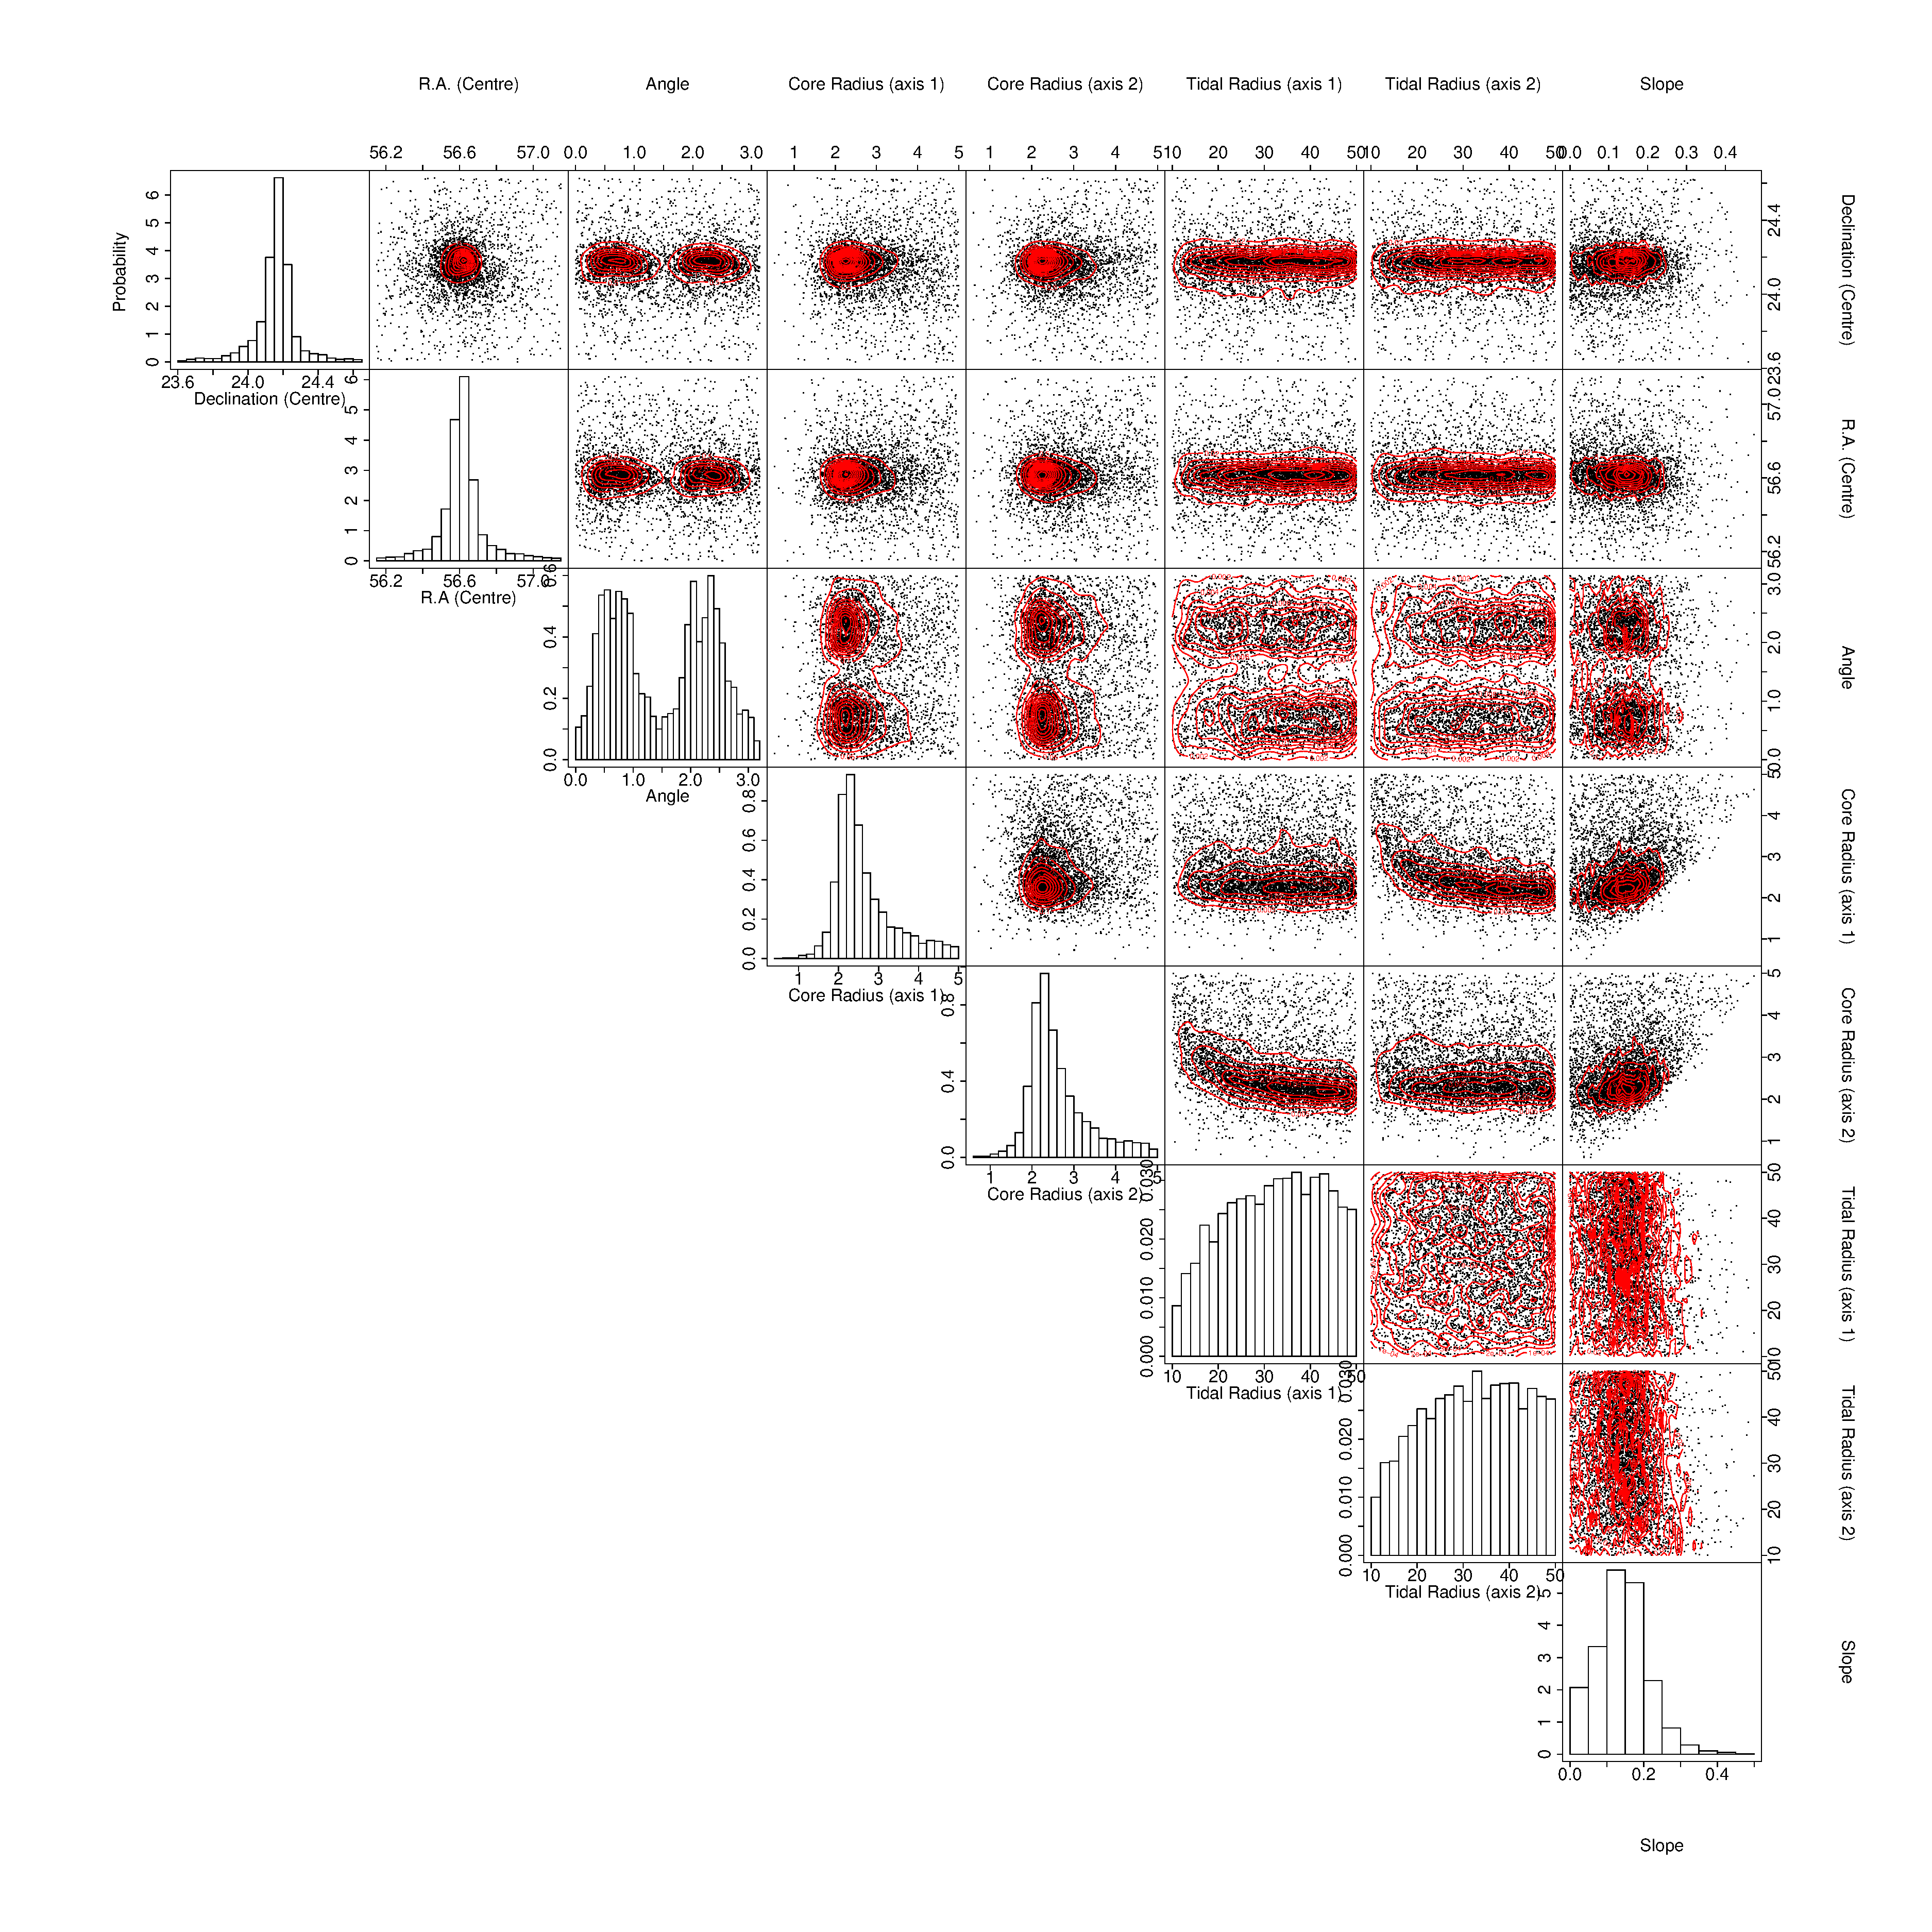
\includegraphics[width=\textwidth]{background/Figures/PSD/KingBS7.pdf}
  \caption{Samples of the posterior distribution of the parameters in the biaxial symmetric and luminosity segregated King model inferred from the 3$^{\circ}$ sample. The core and tidal radius are in units of pc, the slope in units of pc per magnitude.}
\label{fig:KingBS7}
\end {figure}

Finally, combining the evidences and Bayes factors of the King's classical and extended models, we can conclude that there is \emph{decisive} (in terms of Jeffrey's scale) evidence, from both the 3$^{\circ}$  and 6$^{\circ}$ data sets, supporting complex models with J-band luminosity segregation and biaxial symmetry (see Table \ref{tab:BayesFactorsAll}).

\begin{table}[ht!]
  \centering
  \caption[]{Natural logarithm of the evidences (diagonal) and Bayes factors (off-diagonal, computed as in Table \ref{tab:BayesFactors3deg}) for King models with radial symmetry (King-R), biaxial symmetry (King-B), and radial and biaxial symmetry with luminosity segregation (\gls{krs} and \gls{kbs}, respectively). These evidences are computed using the samples of $3^{\circ}$ and $6^{\circ}$.}
  {\small 
\begin{tabular}{cc|cccc|cccc}
\hline              
\hline              
&&  \multicolumn{4}{c}{$3^{\circ}$} &   \multicolumn{4}{c}{$6^{\circ}$} \\
\hline              
&&King-R& King-B &  King-RS& King-BS & King-R & King-B& King-RS &  King-BS \\
\hline              
\multirow{4}{*}{$3^{\circ}$} &King-R&-2876.2&$>100$&2.01&$>100$&&&&\\
&King-B&&-2806.9&$<0.1$&20.1&&&&\\
&King-RS    & & &-2875.5   & $>100$&          &           &    &        \\
 &King-BS &    &   &     &  -2803.9  &   &&        &           \\
 \hline
\multirow{4}{*}{$6^{\circ}$}&King-R   && &&            & -5033.5          & $>100$  & $>100$&  $>100$  \\
&King-B&&&&&&-5023.8&0.2& $>100$\\
&King-RS &&&&            &           &         & -5025.4  &   $>100$  \\
&King-BS &&&&            &           &         &  &  -5016.4   \\
\hline              
         \end{tabular}
         }
\label{tab:BayesFactorsAll}
\end{table}

The results of this Section show that, although the majority of the current models of the radial density profile of the Pleiades cluster reproduce well the observed data, only the classical King's profile and the \gls{rgp} have the best evidences both in the complete $3^\circ$ sample and in the extended $6^\circ$ one. However, we discard the \gls{rgp} profile due to its high degeneracy and unphysical values. We can perform this selection by the inclusion of restrictive priors \glspl{pdf} to the physical interpretability of the models. This model selection process using non-identical priors for the competing models is explained in Section \ref{sect:modelselection} (see Eq. \ref{eq:modelselection}). 

Also, we have shown that the high membership probability samples, both complete ($3^\circ$) and extended ($6^\circ$), are better modelled, in terms of the evidence, with complex models including biaxial symmetry and luminosity segregation.

The results of this Section establish a solid probabilistic background for: i) the classical King profile, at least in the Pleiades cluster, and ii) luminosity segregation. The latter indicates that the expected mass segregation in the Pleiades cluster \cite[as has been indicated by previous studies, e.g.][]{Converse2010} is supported by Bayesian evidence. 


%%%%%%%%%%%%%%%%%%%%%%%%%%%%%%%%%%%%%%%%%%%%%%%%%%
\section{Proper motions distribution}
\label{sect:PMresults}
The bivariate proper motions distributions of both single and \gls{emb} is directly recovered by the \gls{bhm} by means of the posterior distributions of the parameters in the \gls{gmm} modelling these populations.
These bivariate distributions are depicted in Fig, \ref{fig:PM}.

The univariate projections of these distributions, in the $\mu_{\alpha}\cdot cos(\delta)$ and $\mu_{\delta}$ components, are shown in Figs. \ref{fig:PMCs} and \ref{fig:PMBs}. Also, I show in this figures the densities in the same proper motions projections of the candidate members of \citet{Bouy2015}, and those found by \gls{bhm}, which have membership probabilities grater than 0.84. Interestingly, the densities rendered by both samples of members are almost identical. Nevertheless, the density resulting from the sample of the posterior distributions of the parameters in the \glspl{gmm}, differ from the kernel density estimations of the corresponding populations. This difference results from the distinct populations of the two distributions. The \gls{bhm} finds the posterior distribution of its parameters using the likelihood of all the objects in the data set. The contribution that individual objects have to the total cluster likelihood can be thought to be proportional to their cluster membership probability. Therefore, the observed difference results from those objects whose cluster membership probability is lower than 0.84. The expected number of cluster members in the probability range 0-0.84 amounts to the non negligible value of $\sim 1100$ objects. These objects contaminate the posterior distribution of the parameters in the \gls{bhm} with an expected value of 5.3\% (see Section \ref{sect:classifier}). Nevertheless, within them also lies a 10\% of true cluster members (as estimated in Section \ref{sect:classifier}). Discarding these true cluster members from the statistical analysis will render it biased. Instead, we decided to include these 10\% possible true cluster members at the small price of a 5.3\% of contamination.

\begin{figure}[ht!]
\begin{center}
\includegraphics[page=2,width=\textwidth]{background/Figures/BHM/MembersModel.pdf}
\caption{Proper motion distributions recovered by the \gls{bhm}. The dashed and dot-dashed ellipses represent the mode of 100 samples (orange lines) from the posterior covariance matrices in the cluster and \gls{emb} \glspl{gmm}, respectively. Reproduced from Figure 8 of \citet{Olivares2017},\textit{\usebibentry{Olivares2017}{Title}}, \usebibentry{Olivares2017}{Journal}, Vol. \usebibentry{Olivares2017}{Volume}.}
\label{fig:PM}
\end{center}
\end{figure}

\begin{figure}[ht!]
    \centering
    \begin{subfigure}[t]{0.45\textwidth}
    \centering
       \includegraphics[page=2,width=\textwidth]{background/Figures/BHM/Cs_members.pdf}
        \caption{}
    \end{subfigure}
    \begin{subfigure}[t]{0.45\textwidth}
    \centering
     \includegraphics[page=3,width=\textwidth]{background/Figures/BHM/Cs_members.pdf}
        \caption{}
    \end{subfigure}
\caption{Proper motions densities resulting from: a 100 element sample from the posterior distributions of parameters in the \gls{gmm} modelling the single stars (orange spaghetti lines), the kernel density estimation of the \gls{bhm} candidate members classified as single stars (those whose cluster membership probability is higher than 0.84 and \gls{emb} membership probability is lower than 0.5), and, the kernel density estimation of the candidate members of \citet{Bouy2015} whose photometry lies below the \gls{emb} sequence (blue line).}
\label{fig:PMCs}
\end{figure}

\begin{figure}[ht!]
    \centering
    \begin{subfigure}[t]{0.45\textwidth}
    \centering
       \includegraphics[page=2,width=\textwidth]{background/Figures/BHM/Bs_members.pdf}
        \caption{}
    \end{subfigure}
    \begin{subfigure}[t]{0.45\textwidth}
    \centering
     \includegraphics[page=3,width=\textwidth]{background/Figures/BHM/Bs_members.pdf}
        \caption{}
    \end{subfigure}
\caption{Proper motions densities resulting from: a 100 element sample from the posterior distributions of parameters in the \gls{gmm} modelling the \gls{emb} stars (orange spaghetti lines), the kernel density estimation of the \gls{bhm} candidate members classified as \gls{emb} stars (those whose cluster membership probability is higher than 0.84 and \gls{emb} membership probability is higher than 0.5), and, the kernel density estimation of the candidate members of \citet{Bouy2015} whose photometry lies near the \gls{emb} sequence (blue line).}
\label{fig:PMBs}
\end{figure}

\section{Luminosity distribution}
\label{sect:luminosity}
This Section describes the process to obtain the $J,H$, and $K_s$ absolute magnitude distributions from the posterior distributions of the parameters in the \gls{bhm}. Later, I compare them to those found by \citet{Bouy2015}, in the $K_s$ band specifically. As in the previous section, I also compare these distributions with those resulting from the kernel density estimates of the candidate members of the \gls{bhm}.

\subsection{Derivation of the magnitude distributions}
\label{subsect:deriveluminosity}
To derive the $J,H,K_s$ magnitude distributions, I first transform the true $\gls{ci}$ distribution into the $J,H,K_s$ apparent magnitude distributions. In this transformation, the fractions of \gls{emb} must be taken into account. To do this, the magnitude distributions of both single and \gls{emb} populations are mixed according to their fractions. In the following paragraphs, I describe the process to obtain the $K_s$ apparent magnitude. This process is similar for the rest of the bands. 

Since we aim at the probability distribution of $K_s$, and it depends on the true $\gls{ci}$, I use this as a nuisance parameter that I later marginalise. Thus, 

\begin{align}
p(K_s | \boldsymbol{\theta}_c) & = \int p(K_s,CI | \boldsymbol{\theta}_c) \cdot dCI =  \int p(K_s | CI ,\boldsymbol{\theta}_c) \cdot p(CI|\boldsymbol{\theta}_c)\cdot \mathrm{d}CI. \nonumber
\end{align}

The term $p(K_s | CI ,\boldsymbol{\theta}_c)$ represents the probability of $K_s$ given the true $\gls{ci}$ and the cluster parameters $\boldsymbol{\theta}_c$. It is given by Eq. \ref{eq:lik-seq}. The second term, $p(CI|\boldsymbol{\theta}_c)$ corresponds to the \gls{gmm} modelling the distribution of the true $\gls{ci}$, it is given by Eq. \ref{eq:colordist}. 

We include the \gls{emb}  distribution with an amplitude equal to their fraction, $1-\pi_{CB}$. Thus,

\begin{align}
p(K_s | \boldsymbol{\theta}_c) & =  \int \left[\pi_{CB}\cdot p_{Cs}(K_s| CI, \boldsymbol{\theta}_c) + (1-\pi_{CB})\cdot p_{Bs}(K_s| CI, \boldsymbol{\theta}_c)\right]\nonumber \\& \cdot p(CI|\boldsymbol{\theta}_c)\cdot \mathrm{d}CI. \nonumber \\
& =   \pi_{CB} \int p_{Cs}(K_s| CI, \boldsymbol{\theta}_c) \cdot p(CI|\boldsymbol{\theta}_c) \mathrm{d}CI \nonumber \\
&+ (1-\pi_{CB})\int p_{Bs}(K_s| CI, \boldsymbol{\theta}_c) \cdot p(CI|\boldsymbol{\theta}_c)\cdot  \mathrm{d}CI. \nonumber \\
\end{align}

In this equation, $Cs$ and $Bs$ are the subindices used to distinguish the probability of $K_s$ under the cluster and \gls{emb} photometric models, respectively. These probabilities are defined for the vector of photometric measurements, $\boldsymbol{d}_{ph}$ (see Eq. \ref{eq:lik-seq}). Since we are interested only in the distribution of $K_s$ (by now), we marginalise the rest of the photometric entries,including the observed $\gls{ci}$ (I use a tilde over the observed quantities). Also, the integration limits must change to those of the truncated true colour distribution ($\gls{ci}_{min}=0.8, \gls{ci}_{max}=8$). Hence,

\begin{align}
&p(K_s | \boldsymbol{\theta}_c)  =   \pi_{CB} \int_{CI_{min}}^{CI_{max}}\left[ \left[\sum_{i=1}^5 \pi_{CI,i} \cdot \mathcal{N}_t(CI| \mu_{CI,i},\sigma_{CI,i})\right]\right. \nonumber \\
&\cdot  \left.\int_{\tilde{CI},\tilde{Y},\tilde{J},\tilde{H}}\mathcal{N}(\{\tilde{CI},\tilde{Y},\tilde{J},\tilde{H},K_s\}|\boldsymbol{\mathcal{S}}(CI, \boldsymbol{\beta}),\Sigma_{clus})~\mathrm{d}\tilde{CI}~\mathrm{d}\tilde{Y}~\mathrm{d}\tilde{J}~\mathrm{d}\tilde{H}\right] \cdot \mathrm{d}CI \nonumber \\
& + (1-\pi_{CB}) \int_{CI_{min}}^{CI_{max}}\left[\left[\sum_{i=1}^5 \pi_{CI,i} \cdot \mathcal{N}_t(CI| \mu_{CI,i},\sigma_{CI,i})\right]\right.\nonumber\\
&\cdot \left. \int_{\tilde{CI},\tilde{Y},\tilde{J},\tilde{H}}\mathcal{N}(\{\tilde{CI},\tilde{Y},\tilde{J},\tilde{H},K_s\}|T_{Bs}(\boldsymbol{\mathcal{S}}(CI, \boldsymbol{\beta})),\Sigma_{clus})~\mathrm{d}\tilde{CI}~\mathrm{d}\tilde{Y}~\mathrm{d}\tilde{J}~\mathrm{d}\tilde{H}\right]\cdot \mathrm{d}CI. \nonumber 
\end{align}

The derivations of the $J$ and $H$ magnitude distributions are similar. Since this process takes into account the unresolved \gls{emb} and the so called single stars, which in fact could be binaries with low mass ratios, then I call these distributions the apparent system magnitude distributions. 

The previous distributions, together with the parallax and extinction of the cluster, are used to obtain the luminosity distributions, more properly the absolute system magnitude distributions. I assume that the distribution of parallaxes of the Pleiades members is normally distributed with mean, $7.44$ mas, and standard deviation $0.42$ mas \citep{Galli2017}. Then, to obtain the absolute magnitude distributions, I subtract this parallax distribution, by means of a convolution, to the $J,H,K_s$ magnitude distributions. Finally, I deredden the previous distributions employing the canonical value of extinction for the Pleiades: $A_v=0.12$ mag \citep{Guthrie1987}. This last values were transformed into the $J,H,K_s$ extinctions using the extinction law of \citet{Cardelli1989}.

The completeness limits of the derived luminosity distributions are acquired as follows. Since the \gls{bhm} methodology prescribes the \emph{true} photometric quantities based on the \emph{true} colour index $\gls{ci}$. Then, the completeness limits of the $\gls{ci}$ distribution dictate those of the luminosity distributions. 

\citet{Bouy2015} mention that, due to the heterogeneous origins of the \gls{ddr2} data set, the spatial coverage and sensitivity of the survey is also not homogeneous. To remedy this issue, they identify a region with complete spatial coverage, the inner three degrees of the cluster (see Fig. \ref{fig:originDANCeDR2}). Then, they restricted their photometric analysis to this spatially complete region. 

Restricting their sample of candidate members to this inner region results in a sample of candidate members that is spatially biased. If any dynamical process has been set on the cluster such that the mass distribution of its members is not uniformly distributed in the space, then a spatial cut in a sample of candidate members will result in a bias on the mass distribution. One of such dynamical process is the mass segregation, which, as suggested by \citet{Adams2001} may have happen in the Pleiades cluster. As proven in Section \ref{sect:lumsegregation}, there is strong evidence in favour of luminosity segregation in the Pleiades, at least in the $J$ band.

Thus, to avoid such biases, I assume that the UKIDSS survey, which is the most profound from among the contributions to the \gls{ddr2} data set, provides the homogeneous spatial and sensitivity coverage at faint magnitudes (see Fig. \ref{fig:originDANCeDR2}). This survey thus provides the upper completeness limits, which are essentially those reported in the Appendix A of \citet{Bouy2015}, $i\sim23$ mag and $K_s\sim18$ mag.

Since we are interested in the completeness limits of the $\gls{ci}$, and this equals $i -K_s$, then its completeness limits are defined by those of $i$ and $K_s$ together. In Fig. \ref{fig:completeness}, I show the $K_s$ and $i$ kernel density estimate computed using all sources in the \gls{ddr2}. As can be seen from this Figure, the point with maximum density, which corresponds to $i=21.4$ mag and $K_s=18.1$ mag, should be used to set the upper completeness limits. Notice that, due to the use of the two dimensional density, the upper completeness limit in $i$ is reduced with respect to that of the univariate $i$ distribution. This density shows a sharp decline at bright magnitudes, probably due to saturation of the detectors. To be conservative, I choose $i=13.2$ mag and $K_s=11.0$ mag as the lower completeness limits.

\begin{figure}[htbp]
\begin{center}
\resizebox{\hsize}{!}{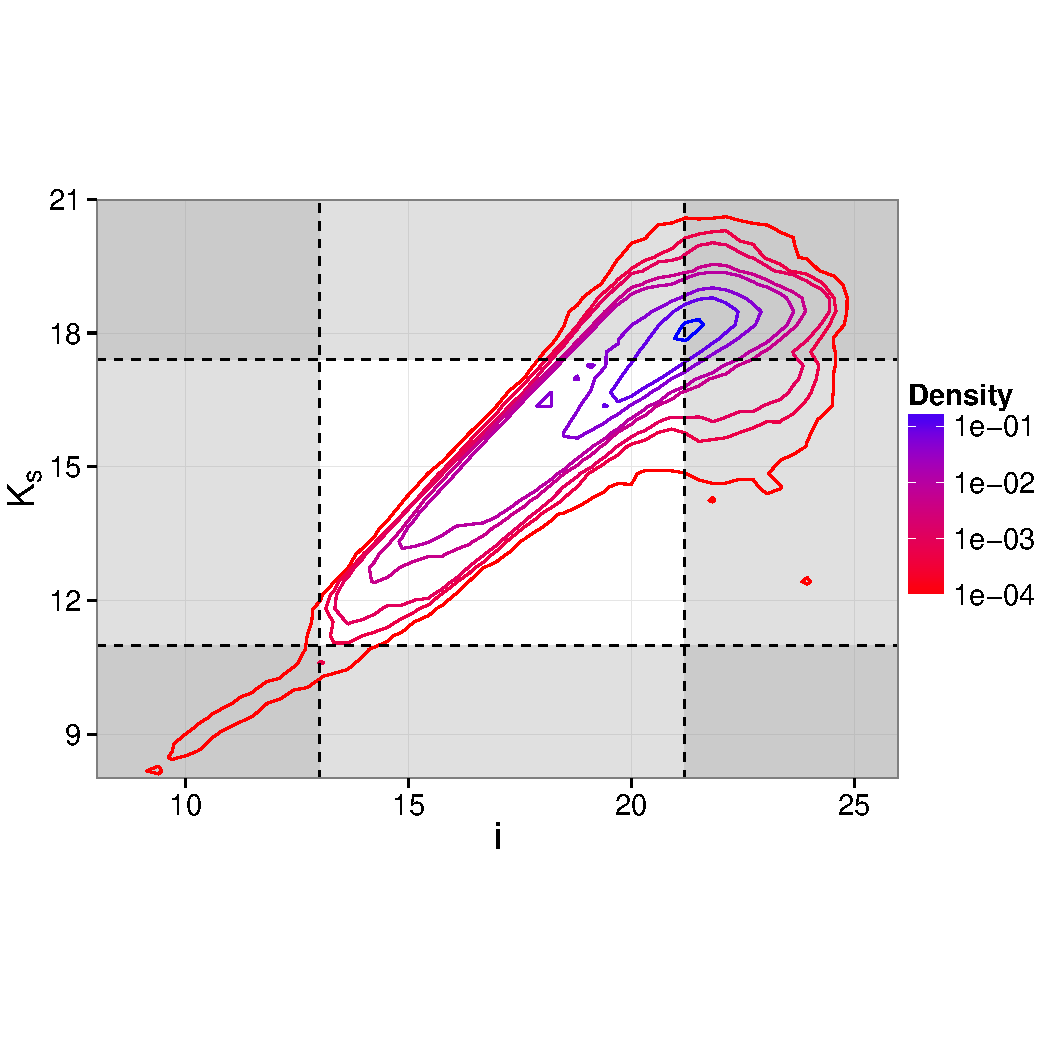
\includegraphics[width=0.8\textwidth]{background/Figures/Density-Kvsi.pdf}}
\caption{Density of all \gls{ddr2} sources in $K_s$ and $i$ magnitudes. Lines show the chosen completeness limits, $13.2<i<21.4$ mag and $11<K_s<18.1$ mag. The grey area is considered incomplete. Reproduced from Figure 9 of \citet{Olivares2017},\textit{\usebibentry{Olivares2017}{Title}}, \usebibentry{Olivares2017}{Journal}, Vol. \usebibentry{Olivares2017}{Volume}.}
\label{fig:completeness}.
\end{center}
\end{figure}

The $\gls{ci}$ completeness interval is then defined as that of all the points, along the cluster sequence in the $K_s$ vs. $i-K_s$ \gls{cmd}, for which $i$ and $K_s$ are bounded by their upper and lower completeness limits, respectively. This results in a completeness interval of  $2.7<\gls{ci}<5.6$ mag. With it, and the cluster sequence (the splines), I derive the completeness intervals for the $J,H,K_s$ bands. Finally, I transform these intervals to absolute magnitudes and deredden them. 

The luminosity distributions of the $J,H,K_s$ bands, together with their completeness limits are shown in Fig. \ref{fig:Luminosities}. I call them model \gls{bhm}. For the sake of comparison, I also show the following luminosity distributions. First, the luminosity distributions of objects classified as candidate members in the \gls{bhm}. I call these the discrete \gls{bhm} distributions. Also, I plot the luminosity distribution resulting from the candidate members of \citet{Bouy2015}, I call them the discrete Bouy. Since the discrete luminosity distributions, both Bouy and \gls{bhm}, rely on the magnitudes of the individual candidate members, and many of these objects have missing value entries, then I impute their missing entries using those of the nearest euclidean neighbour. 

The difference between the luminosity distributions derived using the posterior distribution of the parameters in the \gls{bhm} and discrete \gls{bhm} distributions, comes as well from the fact that the candidate members are not a random sample of the cluster population. As explained before, the luminosity distributions derived from the parameters in the model take into account all objects proportionally to their cluster membership probability. The discrete \gls{bhm} uses only the high probability candidate members, thus they may be biased by the probability threshold. In addition, the missing value entries of al the objects in the model \gls{bhm} distributions are marginalised, while in the discrete \gls{bhm} they are imputed.
 
On the other hand, the differences between the discrete distributions, the \gls{bhm} and that of \citet{Bouy2015}, arise mainly at the bright and faint ends ($K_s\sim 4$ mag and $K_s\sim11$ mag). I hypothesise that the origin of these differences lie in the different list of candidate members. As it has been discussed, the model of \citet{Bouy2015} is constructed only based in fully observed objects. The regions where the objects with missing entries happen more frequently is in the bright and faint regions. Therefore, the observed differences in the luminosity distributions may arise from the incomplete treatment that those authors made of objects with missing entries.

\begin{figure}[htbp]
\begin{center}
\resizebox{\hsize}{!}{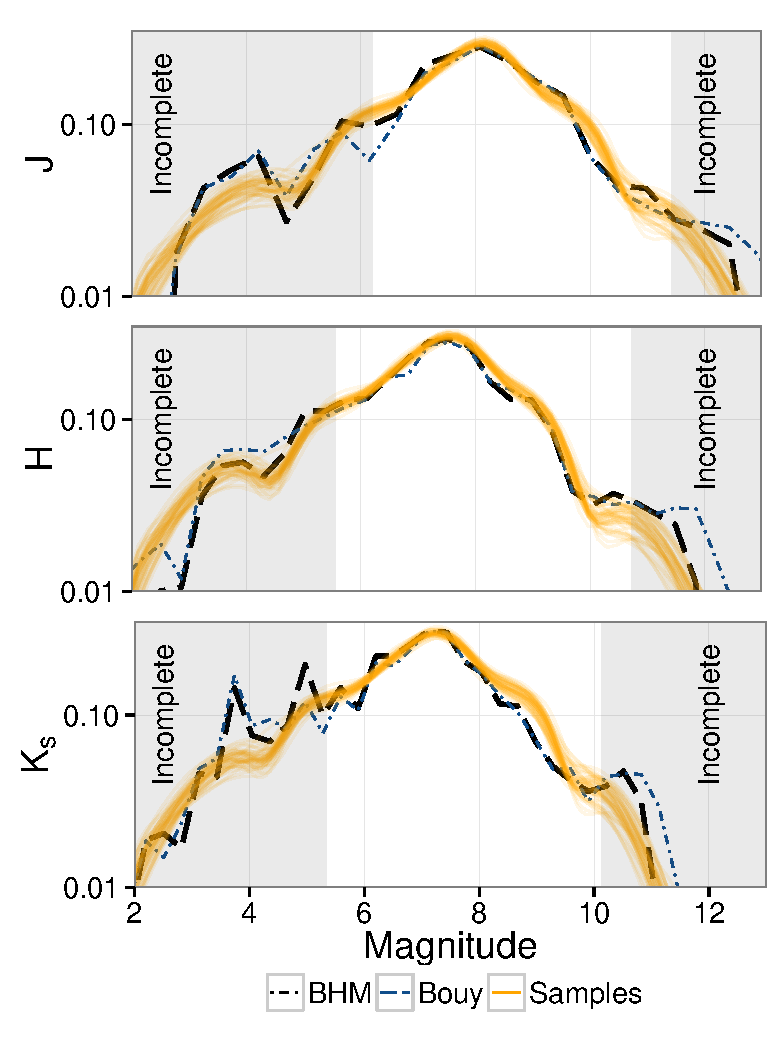
\includegraphics[width=0.8\textwidth]{background/Figures/BHM/absolute_JHK-log.pdf}}
\caption{Luminosity distribution of $J,H,K_s$ bands (orange spaghetti lines). Also shown: the regions of incompleteness, and, the luminosity distributions computed from: the candidate members of \citet{Bouy2015} (dot-dashed blue line), and our candidate members, ($p_{84\%}>p_t$, dashed black line). Reproduced from Figure 10 of \citet{Olivares2017},\textit{\usebibentry{Olivares2017}{Title}}, \usebibentry{Olivares2017}{Volume} \usebibentry{Olivares2017}{Volume}.}
\label{fig:Luminosities}.
\end{center}
\end{figure}

\section{Mass distribution}
\label{sect:massdistributionresults}

In this Section I describe the procedure to transform the luminosities distributions into mass distributions. Transforming a  probability distributions requires the transformation \emph{per se} and its derivative (see Section \ref{sect:introprobability}). Once the mass distributions is obtained,  then, I compare it to the \glspl{imf} of \citet{Chabrier2005} and \citet{Thies2007}. Finally, I conclude this section with the analysis of some simple toy models that can be fitted to the derived mass distribution.

\subsection{The mass-luminosity relation}
\label{sect:mass-luminosity}
The mass-luminosity relation is the non linear transformation that enables us to obtain the mass distribution from the luminosity distributions. Given the values of the upper limits of the luminosity distributions (the faint ends), the mass-luminosity relation relies entirely on the current models of stellar atmospheres. Among the different flavours of theoretical stellar evolution models in the literature (those from the Pisa, Padova, Trieste, Geneva, and Lyon research groups)  we choose the BT-Settl models of \citet{Allard2012}. These models go deeper into the lower masses reaching the planetary mass range thus allowing a complete coverage of our luminosity distributions. The rest of the models stay in the $0.1-10\,\mathrm{M_{\odot}}$ range, with the \emph{PARSEC} models being the ones reaching the $0.1\,\mathrm{M_{\odot}}$ limit \citep{Bressan2012}. 

From the BT-Settle grid I choose the CIFIST2011bc for the 2MASS AB photometric system, 120 \gls{myr} and solar metallicity. I choose this photometric system because it covers the dynamic range of the \gls{ddr2} survey. The age and metallicity values are the closest, within the grid, to the canonical ones (see Section \ref{sect:generalities}). This grid returns values of the luminosity for certain non uniformly distributed values of the mass. As shown in Eq. \ref{eq:transformdistribution}, the transformation of a probability distribution, in this case the luminosities, into the mass distribution is proportional to the derivative of the transformation, which must be continuous. To avoid the discontinuities in the derivatives produced by the grid, we fit the values from the grid using spline series (see Fig. \ref{fig:splineML}). Then, derivative is obtained from these continuous series (see Fig. \ref{fig:der_splineML}). It is important to notice the following two assumptions. First, I assume that the luminosity distributions in $J,H$ and $K_s$ bands are independent between them, and then I obtain a mass distribution for each one of them. Second, I assume that the transformation from luminosities to masses does not have any associated uncertainty. These assumptions must be taken since the isochrone models do not provide neither uncertainties nor a way to incorporate correlations between the mass distributions of distinct photometric bands. 

Figure \ref{fig:splineML} shows the spline fit to the mass-luminosity relations of the BT-Settl absolute $J,H$ and $K_s$ magnitudes (black points) as a function of the mass. Figure \ref{fig:der_splineML} shows the derivative of mass-luminosity relation. The grey shaded areas represent the incompleteness regions of the \gls{dance} survey (see previous section).

\begin{figure}[ht!]
    \centering
    \begin{subfigure}[t]{0.7\textwidth}
    \centering
       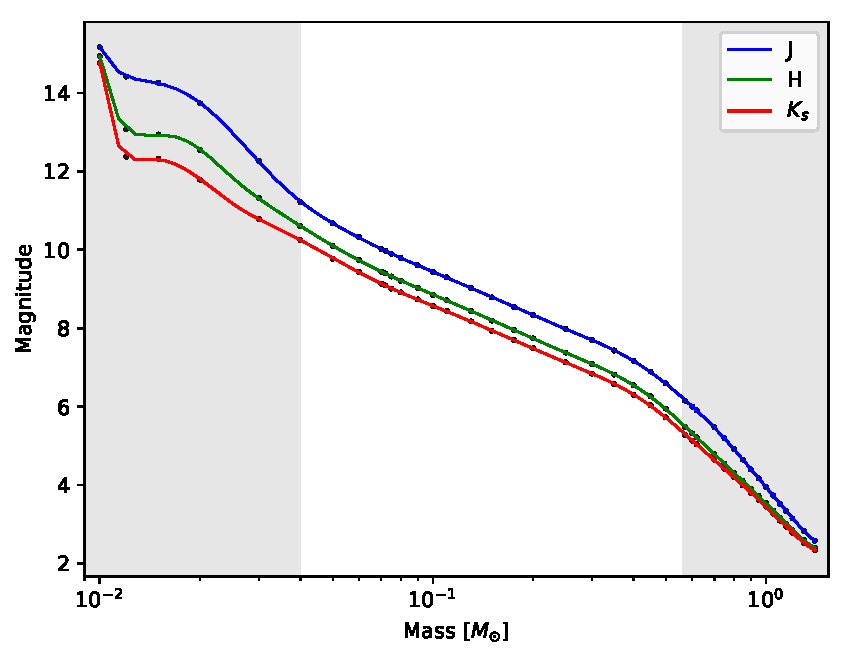
\includegraphics[page=1,width=\textwidth]{background/Figures/FitSpline_AllardModels.pdf}
        \caption{}
        \label{fig:splineML}
    \end{subfigure}
    \begin{subfigure}[t]{0.7\textwidth}
    \centering
     \includegraphics[page=2,width=\textwidth]{background/Figures/FitSpline_AllardModels.pdf}
        \caption{}
        \label{fig:der_splineML}
    \end{subfigure}
\caption{Upper panel: Mass-luminosity relations from the BT-Settl models \citep{Allard2012} for the $J, H$ and $K_s$ bands of the \emph{2MASS} photometric system (black dots). Also shown, the splines fitted to the previous relations. Bottom panel: The derivative of the mass-luminosity relations in the upper panel. The incompleteness regions of the \gls{dance} survey (grey areas) are shown in both panels.}
\label{fig:ML}
\end{figure}

\subsection{Present day system mass distribution}

The mass distribution is independently obtained for the $J,H,K_s$ luminosity distributions by means of the mass-luminosity relations described in the previous section. Since the luminosity functions of Sect. \ref{sect:luminosity} correspond to the luminosity of systems (single stars unresolved binaries and multiple systems), then, the derived mass function corresponds to the \glsfirst{pdsmd}.  Figure \ref{fig:MassDistribution} shows the logarithmic \gls{pdsmd} ($\xi_L$) for the $J,H,K_s$ bands normalised on the completeness limits of the \gls{dance} survey. The logarithmic representation of the mass distribution is a transformation from the natural variable of mass into the logarithm of 10 scale. It is customary to represent the mass distribution in this scale.

\begin{figure}[htbp]
\begin{center}
\resizebox{\hsize}{!}{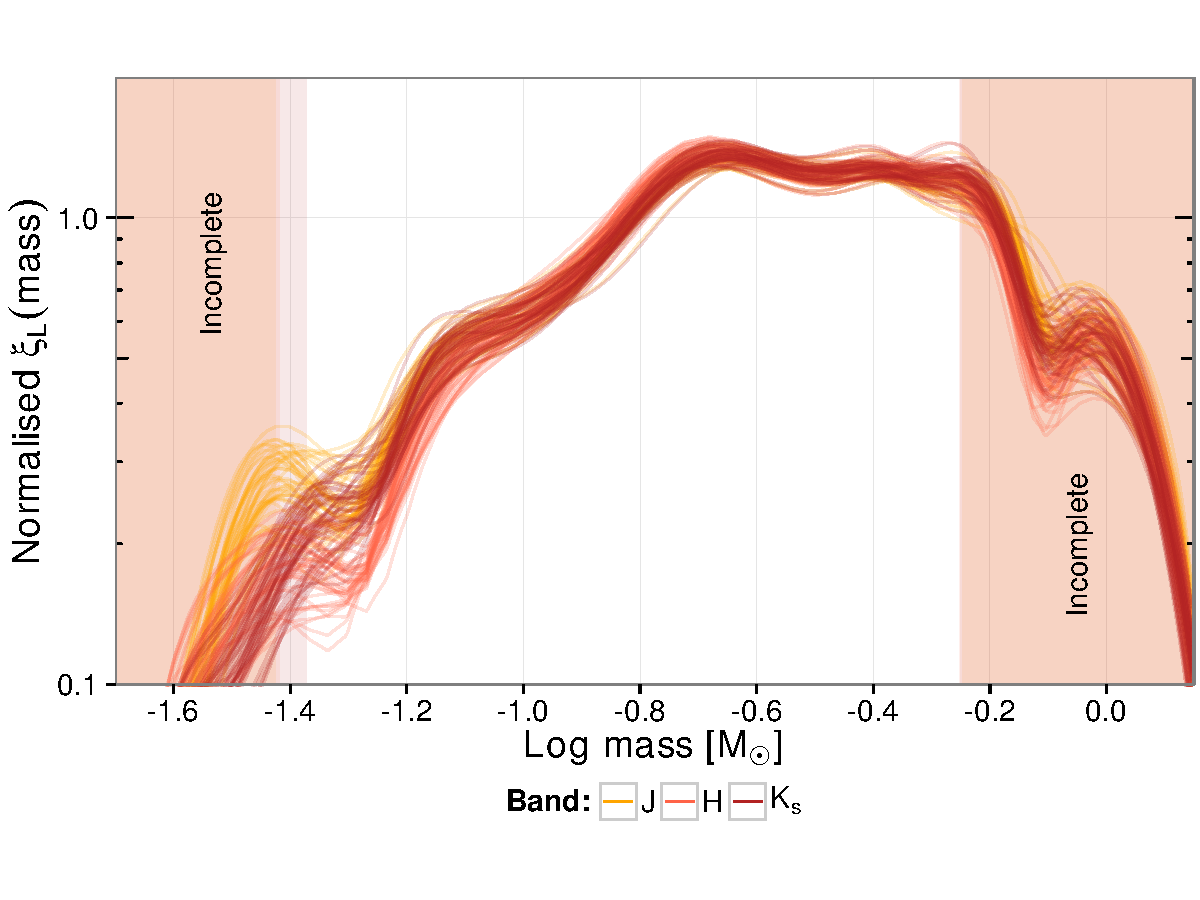
\includegraphics[width=\textwidth]{background/Figures/BHM/MassDistribution.pdf}}
\caption{Normalised logarithmic \gls{pdsmd} in $J,H,K_s$ band. Also shown the completeness limits computed in previous section and transformed with the mass-luminosity relation.}
\label{fig:MassDistribution}
\end{center}
\end{figure}

For the sake of comparison, Figure \ref{fig:ModelMassFunction} shows the \gls{pdsmd} ($\xi_L$) for the $K_s$ band of the previous Figure, together with the three-slope power-law function of \citet{Bouy2015}, and the \gls{imf} of \citet{Thies2007} and \citet{Chabrier2005}. The standard uncertainties in \citet{Chabrier2005} \gls{imf} are those reported in \citet{Chabrier2003b}. 

This Figure shows that the \glspl{pdsmd} derived from the \gls{bhm} compare well, at least in the completeness interval, with the one proposed by \citet{Bouy2015}. The discrepancies between these two, above $0.3 \mathrm{M_{\odot}} (-0.5 < \log \mathrm{M/M_{\odot}})$ particularly, may have its origin on the following aspects.

The \gls{pdsmd} of \citet{Bouy2015} is computed using only their candidate members within the central three degree region of the \gls{ddr2}. First, their list of candidate members is not the same as those found by the \gls{bhm}. Second, the \gls{pdsmd} derived from the \gls{bhm} uses all objects in the data set, not just the high membership probability candidates. Third, as mentioned in Section \ref{sect:luminosity}, the cut to the central three degree region may have biased the derived \gls{pdsmd} of \citet{Bouy2015}. Therefore, the lack of objects that it shows,  in the mass range $0.3 - 0.7 \mathrm{M_{\odot}}$ ($-0.5 < \log \mathrm{M/M_{\odot}} < -0.2$) particularly, may has it origin in the objects that \citet{Bouy2015} did not included in his analysis: those lying outside the inner three degree region. 

For the sake of completeness, I fit a simple model to the \gls{pdsmd} of the \gls{bhm}. To do it, I proceed as follows. First, I select three competing models: a log-normal function (like that of \citet{Chabrier2003b,Chabrier2005}), and two power-law functions of the form $m^{-\alpha}$ with two and three power-law segments. Second, from a 100 sample distribution of the \gls{pdsmd} in the $K_s$ band (the ones shown as spaghetti lines in Fig. \ref{fig:ModelMassFunction}) I compute the mean distribution. This is, at each of the 200 points grid spanning the completeness interval, I obtain the mean of the probabilities given by the 100 distributions. With this mean distribution I draw a $10^4$ synthetic sample of masses. Third, using \emph{PyMultiNest} \citep{Buchner2014}, I infer the parameters of the three models given the masses of the synthetic sample. Table \ref{tab:fitPDSMD} gives the \gls{map} of the parameters in each model together with the natural logarithm of the evidences (see Sect. \ref{sect:modelselection}). Judging by \citet{Jeffreys61} scale of evidence (see Table \ref{tab:JeffreysScale}), there is decisive evidence supporting the two and three segment power-law models. However, the Bayes factor of the latter indicates a difference in evidence which barely worth mentioning. Thus, in the following I compare with the two-segment power-law model that is shown on Fig. \ref{fig:ModelMassFunction} (as the black solid line).

The two segment power-law model agrees with the three segment model of \citet{Bouy2015}. However, there are still differences, which are clear at the low and high mass ends particularly. Nevertheless, it is in clear discrepancy with the \glspl{imf} of \citet{Chabrier2005},  \cite[$m_c=0.25_{-0.016}^{+0.021}$ and $\sigma=0.55_{-0.01}^{+0.05}$, the uncertainties are those reported by][for single objects]{Chabrier2003b} and of \citet{Thies2007}. 

The discrepancy between the \glspl{imf} and the \gls{pdsmd} derived from the \gls{bhm} and the \gls{pdsmd} of \citet{Bouy2015} may have its origin on the not yet established uncertainties in the mass-luminosity relation, on dynamical effects associated with age, or in a combination of the previous. In the next section I compare the \gls{pdsmd} of the Pleiades with that of other younger and older clusters in order to analyse if there is evidence of dynamical effects associated with age.

\begin{table*}[ht!]
\caption{Parameters and evidence of models fitted to the \gls{pdsmd}}
\begin{center}
\begin{tabular}{lll}
Model&Parameters& Log Evidence\\
\hline
LogNormal&$m_c=0.36\pm0.03$&\\
                 &$\sigma=0.46\pm0.02$ & $18.1 \pm 0.1$\\
\hline
Two Segments &$\alpha_0=-0.11\pm0.06$ \ \ $m \in [0.04,0.22\pm0.01]$ & \\ 
&  $\alpha_1=1.13\pm0.1$ \ \ $m \in [0.22\pm0.01,0.56]$&$2222.7\pm0.4$\\
\hline
Three Segments &$\alpha_0=-0.05\pm0.6$ \ \ $m \in [0.04,0.08\pm0.03]$ & \\
                          &$\alpha_1=-0.1\pm0.1$ \ \ $m \in [0.08\pm0.03,0.22\pm0.01]$ & \\ 
                          &$\alpha_2=1.13\pm0.1$ \ \ $m \in [0.22\pm0.01,0.56]$&$2221.2\pm 0.3$\\
\hline
\end{tabular}
\end{center}
\label{tab:fitPDSMD}
\end{table*}%

However, ending this section, I use the \gls{pdsmd} to give a lower limit to the mass of the cluster. Since the \gls{rdr2} data set  still lacks the very low mass range and most of the high mass range, the mass derived from this \gls{pdsmd} is only a lower limit to the mass of the cluster. From the \gls{pdsmd}, the cluster mean mass in the entire mass range is $0.257 \pm 0.006 \mathrm{M_{\odot}}$. Thus, the product of this mean mass with the expected number \footnote{As explained before, the expected number of cluster members is the integral, over the whole range of membership probabilities, of number of objects at each membership probability value.} of cluster members ($3301 \pm 140$), gives the expected mass of the cluster in this mass range. This  value is $845^{+38}_{-33} \mathrm{M_{\odot}}$. 

Finally, I notice that, as mentioned in Sect. \ref{sect:mass-luminosity}, the uncertainties in the mass-luminosity relations are yet to be established. Thus the quoted uncertainties of our mass results are underestimated.

\begin{figure}[htbp]
\begin{center}
\resizebox{\hsize}{!}{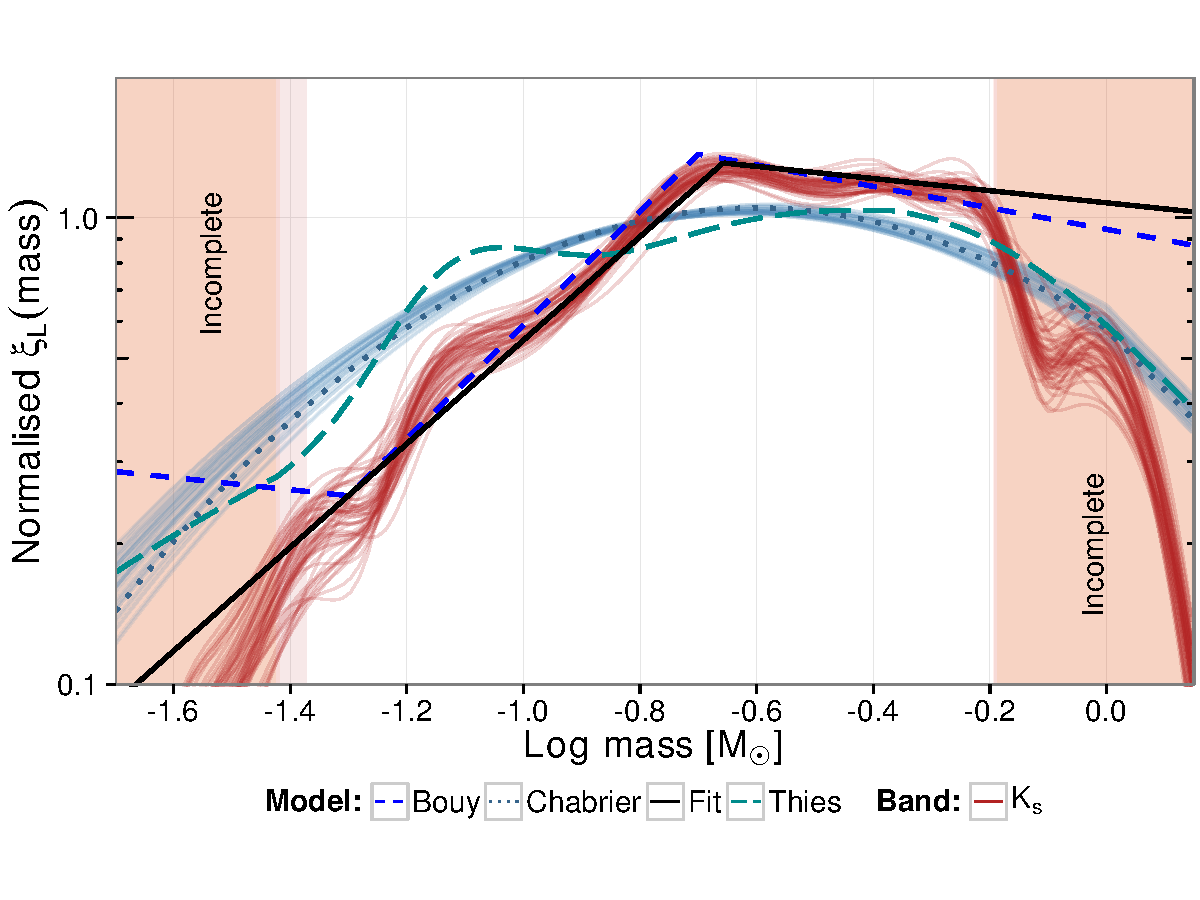
\includegraphics[page=1]{background/Figures/BHM/ModelsMassDistribution.pdf}}
\caption{Normalised logarithmic \gls{pdsmd} in $K_s$ band. Also shown the \glspl{imf} of \citet{Chabrier2005} \cite[blue dotted line with uncertainties from][]{Chabrier2003b} and  \citet{Thies2007} (turquoise long-dashed line), and power-law models found here (black solid line, see text) and by \citet{Bouy2015} (blue dashed line).}
\label{fig:ModelMassFunction}.
\end{center}
\end{figure}

\section{The mass distribution on time}
\label{sect:massontime}
As I mention in the previous section, the observed differences between the present day mass distribution and the initial mass functions may have their origin on the temporal evolution of the cluster population. To test this hypothesis, I compare the Pleiades \gls{pdsmd} ($\sim125$ \gls{myr}) with those of the younger Trapezium ($\sim1$ \gls{myr}) and Hyades ($\sim 600$ \gls{myr}) clusters. These can be thought as snapshots of the Pleiades past and future mass distributions.

Although this comparison formally lies beyond the objectives of the present work, nevertheless, it gives an idea of the importance that the \gls{pdsmd} of other \gls{nyc} have in the understanding of the formation and evolution of the mass distribution.

Figure \ref{fig:PDSMDcomparison} shows the \gls{pdsmd} from the Pleiades, together with those of the Trapezium and Hyades\footnote{Kindly provided by Herv\'e Bouy in a private communication}. These \glspl{pdsmd} correspond to those of  Fig. 11 of \citet{Bouy2015}. As mentioned by \citet{Bouy2015}, the abundance of low-mass stars and brown dwarfs in the range $0.03 - 0.1\,\mathrm{M_{\odot}}(-1.4 < \log \mathrm{M/M_{\odot}} <-1$) seems to diminish with time. The relative increase of objects in the range $-0.4 < \mathrm{\log M/M_{\odot}} < -0.2$ is an effect of the normalisation\footnote{The interesting alternative of open clusters gaining intermediate mass stars is yet to be explored.}. This effect is consistent with the classical scenario in which low-mass stars and brown dwarfs are ejected as the cluster relaxes.

Since I lack the learned \gls{bhm} for these two open clusters, the following comparison is made on a frequentist hypothesis testing approach, rather than on the proper Bayesian model selection scheme.

In this hypothesis test, the null hypothesis is that the Hyades and Trapezium \glspl{pdsmd} came, each of them, from the same distribution than the Pleiades. 

If we want to test the null hypothesis that two distributions come from the same parent distribution, \gls{ks} and the \gls{ad} tests are classical options, with the \gls{ad} the most robust one. To perform these tests, we must compute certain measures from the two distributions. Then, given the measure, the test distribution returns the probability that the two distributions came from the same parent distribution. Finally, we reject the null hypothesis only if the previous probability is lower than certain probability threshold ($\alpha$), which is usually 0.1, 0.05, or 0.01. 

To perform the \gls{ks} tests we must obtain the maximum distance between the \glspl{cdf} of the two distributions. Then, using this distance and the \gls{ks} distribution, we obtain the probability that the two distributions came from the same parent distribution. %If this probability is higher than certain probability threshold ($\alpha$) then the null hypothesis can not be rejected. 

However, the \gls{ks} test can also be applied in a graphical way. Given the $\alpha$ probability threshold, there is a $d_{\alpha}$ distance for which the \gls{ks} distribution returns a probability $\alpha$. For $d < d_{\alpha}$ $p_{KS}(d) > \alpha$ and for $d > d_{\alpha}$ $p_{KS}(d) < \alpha$. Therefore, given the \gls{cdf} of one of the distributions that we want to compare and a probability threshold $\alpha$, the region of distance $d_{\alpha}$ around the \gls{cdf} depicts the hypothesis test. If the \gls{cdf} of the other distribution lies entirely within this region, then its maximum distance from the first \gls{cdf} is less than $d_{\alpha}$. Therefore, its probability is greater than $\alpha$ and the null hypothesis can not be rejected.

\begin{figure}[htp]
\begin{center}
\resizebox{\hsize}{!}{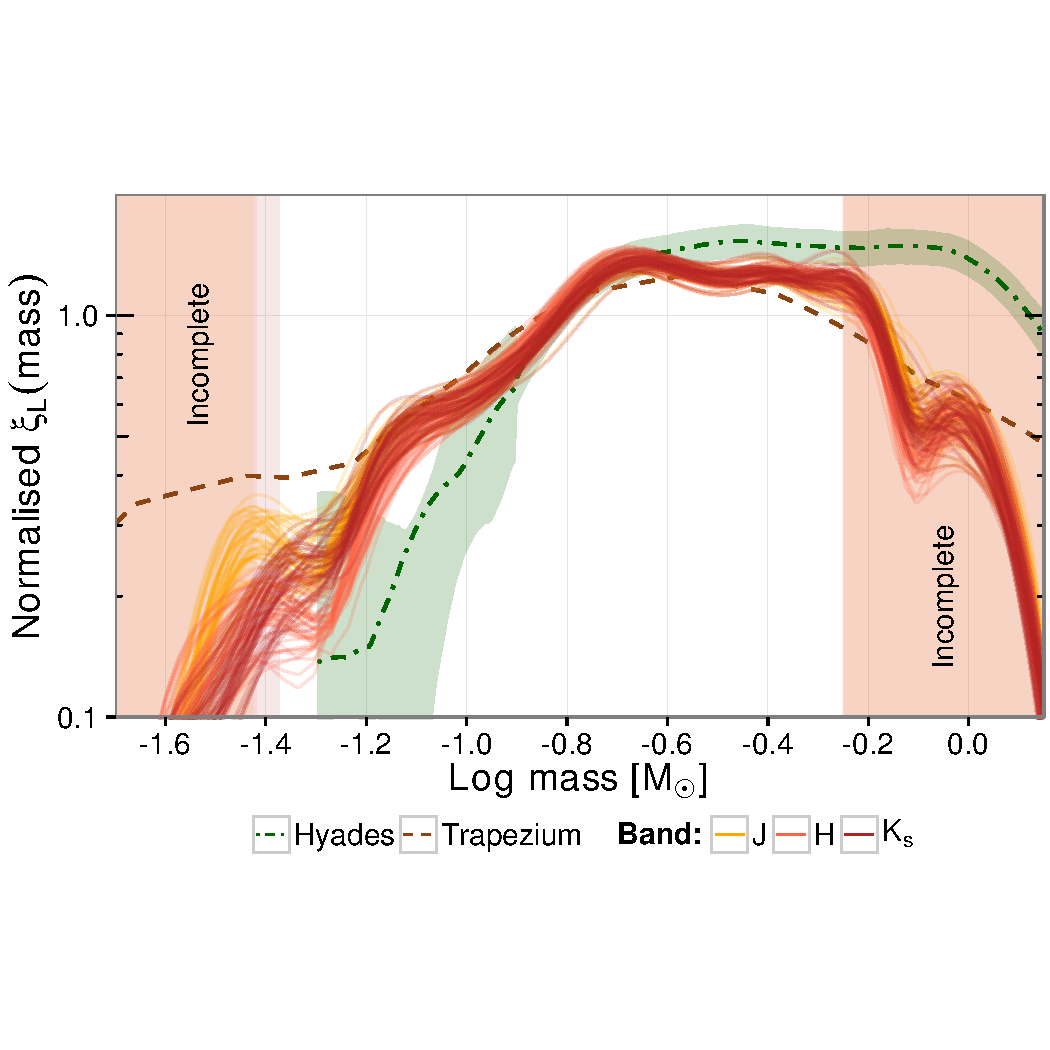
\includegraphics[width=\textwidth]{background/Figures/BHM/M45vsM42vsM44.pdf}}
\caption{The \glspl{pdsmd} of the Pleiades (derived here for $J,H,K_s$ bands), Trapezium, and Hyades (both from \citet{Bouy2015}) clusters. They are normalised in the interval of completeness.}
\label{fig:PDSMDcomparison}.
\end{center}
\end{figure}

\begin{figure}[htp]
\begin{center}
\resizebox{\hsize}{!}{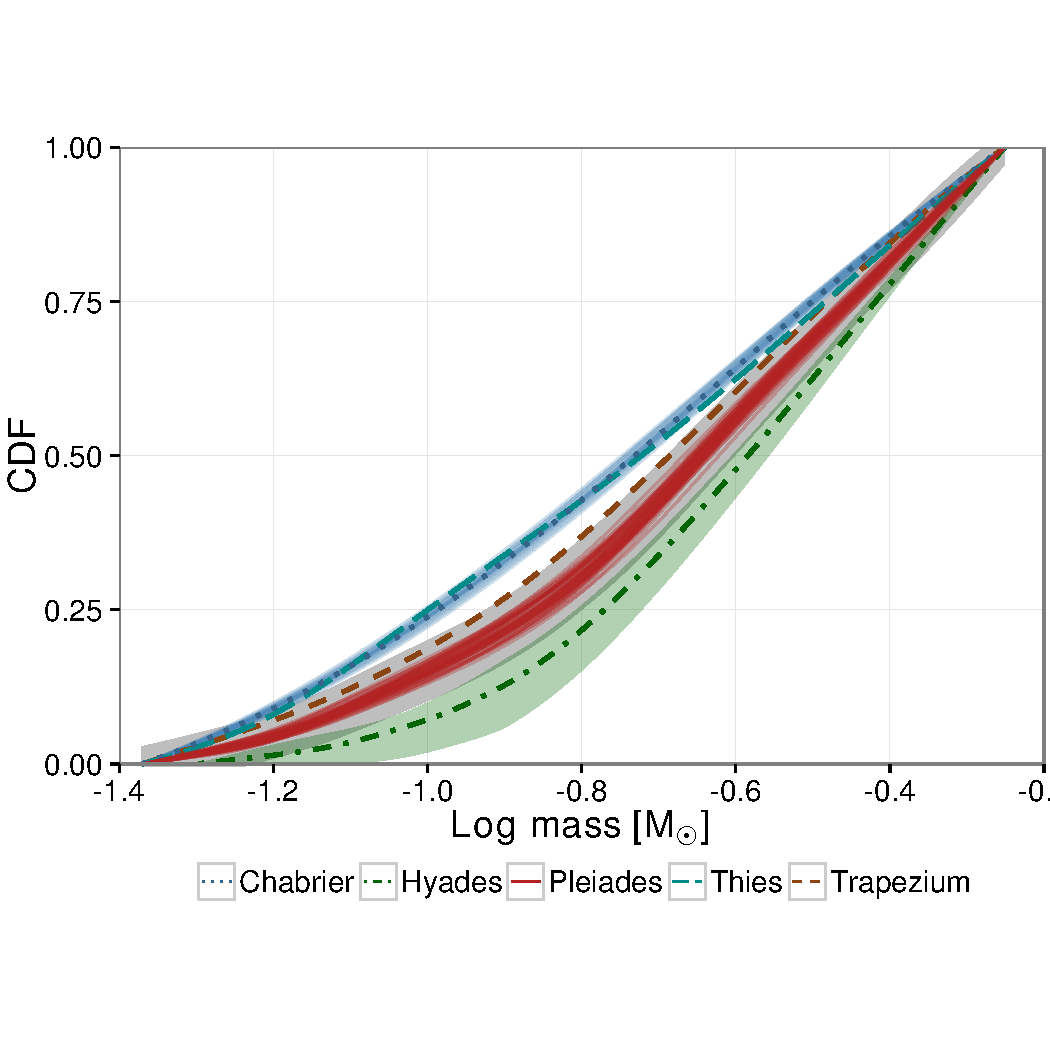
\includegraphics[width=\textwidth]{background/Figures/BHM/CDF_comparison.pdf}}
\caption{\glspl{cdf} of the \glspl{pdsmd} from left panel and that of \citet{Chabrier2005} and \citet{Thies2007} system initial mass function (normalised also in the interval of completeness). The shown Pleiades \gls{cdf} correspond to the $K_s$ band. The grey area depicts the area in which the \glspl{cdf} (both Trapezium and Hyades) should lie for the null hypothesis not to be rejected (at $\alpha=0.01$).}
\label{fig:PDSMDtest}
\end{center}
\end{figure}


Figure \ref{fig:PDSMDtest} shows the cumulative distribution functions (\glspl{cdf}) of the Trapezium, Pleiades (in $K_s$ band) and Hyades \glspl{pdsmd}. Also and for comparison, I show the \glspl{cdf} resulting of \citet{Chabrier2005} and \citet{Thies2007} \glspl{imf}. The grey area around the Pleiades \gls{cdf} depicts the graphical \gls{ks} hypothesis test in which I choose $\alpha = 0.01$.

Furthermore, since the \gls{ks} test uses only the maximum distance between \glspl{cdf}, I also applied the more robust \gls{ad} test. It also rejects the null hypotheses (at $p < 0.004$) that the Trapezium and Hyades \glspl{pdsmd} and the \citet{Chabrier2005} and \citet{Thies2007} \glspl{imf} came from the same parent distribution as the Pleiades \gls{pdsmd}. 

The previous tests suggest that there is enough evidence for the observed differences among the \glspl{pdsmd} of these three clusters. Also, they suggest that \glspl{imf} of \citet{Chabrier2005} and \citet{Thies2007} are statistically different from the  Pleiades \gls{pdsmd}.  These observed differences, as mentioned in the previous Section, may have its origin on dynamical effects associated with age and relaxation.

 Nevertheless, to claim for reliable evidence supporting these differences, several issues must be solved. First, the uncertainties in the \gls{pdsmd} must be properly established. Second, the luminosity distributions must include the uncertainties from the data not just from the poissonian counts. For this, the \gls{bhm} of these cluster must be computed. Finally, the proper way to compare models is under Bayes' theorem.
 




